\documentclass[11pt,a4paper]{article}
\usepackage[T1]{fontenc}
\usepackage[utf8]{inputenc}
\usepackage{lmodern}
\usepackage[margin=28mm]{geometry}
\usepackage{amsmath,amssymb,amsthm,mathtools,mathrsfs}
\usepackage{microtype}
\usepackage{booktabs,longtable,tabularx,array}
\usepackage{graphicx,xcolor,tikz}
\usetikzlibrary{arrows.meta,positioning,calc,decorations.pathreplacing,patterns}
\usepackage[hyphens]{url}
\usepackage[colorlinks=true,linkcolor=blue!45!black,citecolor=blue!45!black,
 urlcolor=blue!45!black,hypertexnames=false]{hyperref}
\usepackage{bookmark}
\allowdisplaybreaks[2]
\setlength{\emergencystretch}{3em}
\setlength{\parskip}{3pt}
\setcounter{tocdepth}{1}
\newtheorem{theorem}{Theorem}[section]
\newtheorem{lemma}[theorem]{Lemma}
\newtheorem{proposition}[theorem]{Proposition}
\newtheorem{corollary}[theorem]{Corollary}
\newtheorem{claim}[theorem]{Claim}
\newtheorem{maintheorem}{Theorem}
\renewcommand{\themaintheorem}{\Alph{maintheorem}}
\theoremstyle{definition}
\newtheorem{definition}[theorem]{Definition}
\newtheorem{example}[theorem]{Example}
\newtheorem{assumption}[theorem]{Assumption}
\theoremstyle{remark}
\newtheorem{remark}[theorem]{Remark}
\newcommand{\R}{\mathbb R}
\newcommand{\T}{\mathbb T}
\newcommand{\av}[1]{\langle #1\rangle}
\newcommand{\dd}{\,d}
\newcommand{\id}{\mathrm{id}}
\newcommand{\supp}{\operatorname{supp}}
\newcommand{\dist}{\operatorname{dist}}
\newcommand{\diag}{\operatorname{diag}}
\newcolumntype{Y}{>{\raggedright\arraybackslash}X}
\hypersetup{pdftitle={Smooth isometric bending of a closed sphere},
 pdfauthor={Boyang Hu}}

\begin{document}
\begin{titlepage}
\centering
\vspace*{.22\textheight}
{\LARGE\bfseries Smooth isometric bending\\[.35em]of a closed sphere\par}
\vspace{2.5em}
{\large Boyang Hu\par}
\vspace{1em}
10 November 2026
\end{titlepage}
\begin{abstract}
A nonradial disk with a rotational metric can rotate inside a fixed
shell without changing that shell's intrinsic metric. The difficulty
is to make the disk exactly planar along its attaching rim. We
construct the required annulus and obtain a smooth embedded sphere
with a smooth periodic isometric bending and noncongruent images.
An inner disk and a complementary cap stay fixed; area, enclosed
volume and total oriented mean curvature stay constant.

The construction starts with a radial infinitesimal deformation.
Infinitely many changes of curvature allow it to reach two flat
ends. Explicit one-dimensional models select one angular mode,
while a mass--resistance description controls the accumulating ends.
Spectral matching and characteristic return maps impose different
nonresonance conditions; both are needed for an inverse on the whole
annulus. Residual corrections put the nonlinear linearizations on
one fixed geometric domain. A Nash--Moser argument then produces an
actual height with flat endpoint extensions. Angular averaging also
gives twice the initial decay exponent for the mean and metric-control
corrections, quantifying how the final metric differs from its radial
reference. The fixed cap supplies the closed bending.
\end{abstract}
\tableofcontents
\clearpage
\section{A closed shell with a moving annulus}
\label{sec:introduction}

Imagine a round disk rotating inside a stationary shell. If the disk
is a surface of revolution, its image does not change. If its height
depends on angle, the image does change, but a rotation will generally
move its attaching boundary. We arrange a third possibility: the
metric is rotational, the embedded disk is not, and a whole collar of
its boundary is planar. An intrinsic rotation followed by the opposite
ambient rotation then fixes the collar pointwise. A stationary cap
closes the disk and turns its relative rotation into a change of shape
of a closed surface.

The geometrical motion is elementary once such a disk exists. Most of
this paper is devoted to its existence, and especially to the exact
flatness required at the attaching collars.

\begin{maintheorem}\label{thm:main}
There are a smooth surface $\Sigma$ diffeomorphic to $S^2$, a smooth
Riemannian metric $g_\Sigma$, and a jointly smooth map
$\mathcal F:\Sigma\times\R\longrightarrow\R^3$ such that, writing
$F_\tau=\mathcal F(\,\cdot\,,\tau)$,
\[
 F_\tau\text{ is an embedding},\qquad
 F_\tau^*g_{\mathrm E}=g_\Sigma,\qquad F_{\tau+1}=F_\tau.
\]
At least two images $F_\tau(\Sigma)$ are not congruent under the
Euclidean isometry group. An inner disk and a complementary cap are
fixed pointwise throughout the family. The area, enclosed volume and
total oriented mean curvature are independent of $\tau$.
\end{maintheorem}

Here a closed surface is compact without boundary. A bending refers
to a family of isometric embeddings of one fixed metric; nontriviality
in this paper always means noncongruence of images, not just motion of
material points. Mean curvature is $(k_1+k_2)/2$, with the outward
orientation. These conventions matter because a relabelling of a
fixed surface is an isometric motion of its material points, but does
not change its shape.

\begin{figure}[htbp]
\centering
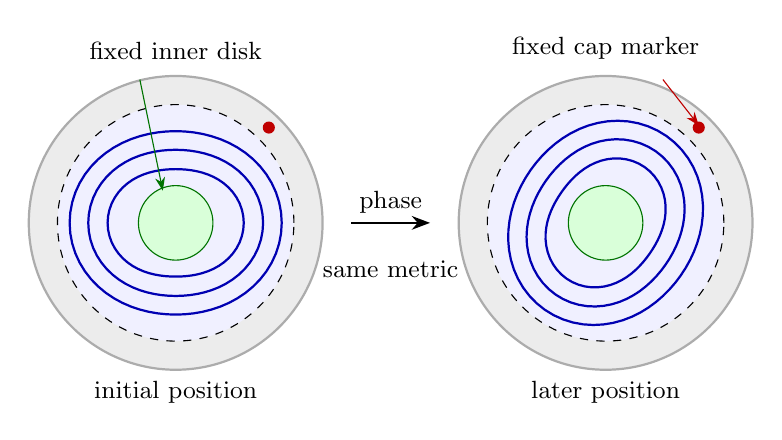
\begin{tikzpicture}[scale=.91,>=Stealth,font=\small]
\foreach \shift/\phase/\word in {0/0/initial,6/55/later}{
 \begin{scope}[xshift=\shift cm]
 \fill[gray!15] (0,0) circle (2.05);
 \fill[blue!6] (0,0) circle (1.65);
 \draw[gray!65,thick] (0,0) circle (2.05);
 \draw[dashed] (0,0) circle (1.65);
 \foreach \radius in {.85,1.12,1.38}{
  \draw[blue!70!black,thick,rotate=\phase]
   plot[domain=0:360,samples=65,variable=\t]
   ({(\radius+.10*cos(2*\t))*cos(\t)},
    {(\radius+.10*cos(2*\t))*sin(\t)});}
 \filldraw[fill=green!15,draw=green!45!black] (0,0) circle (.52);
 \fill[red!75!black] (1.30,1.33) circle (2.4pt);
 \node at (0,-2.36) {\word\ position};
 \end{scope}}
\draw[->,thick] (2.45,0)--(3.55,0);
\node[above] at (3,0) {phase};
\node[below,align=center] at (3,-.4) {same metric};
\node[above] at (0,2.15) {fixed inner disk};
\draw[->,green!45!black] (-.5,2.0)--(-.18,.45);
\node[above] at (6,2.15) {fixed cap marker};
\draw[->,red!75!black] (6.8,2.0)--(7.30,1.36);
\end{tikzpicture}
\caption{Relative rotation, viewed from above. The blue curves are
schematic height contours, not numerical data for the constructed
surface. The circular collars and the green inner disk stay fixed
pointwise. The cap's red marker stays fixed while the nonradial part
turns, so an ambient rotation cannot account for the entire motion.}
\label{fig:surface-motion}
\end{figure}

\subsection{Where the question sits in surface theory}

Ghomi asks whether a closed $C^2$ surface in $\R^3$ can be flexible
in Problem~1.1 of \cite{Ghomi2019}. The problem requires a continuous
family. Replacing a dimple by its reflection across a flat rim gives
two different isometric realizations, but gives no path between them.
Theorem~\ref{thm:main} provides such a path in the smooth category.

The distinction from infinitesimal bending is just as substantial.
A normal vector field supported inside a planar patch has zero first
variation of the metric. This observation already appears in
Cohn-Vossen's discussion of closed infinitesimally nonrigid surfaces
\cite[footnote~2]{CohnVossen1930}. It does not solve the nonlinear
isometry equations. Efimov's classical survey
\cite{Efimov1948Survey} and his work on deformation at zero-curvature
points \cite{Efimov1948Zero} belong to the historical setting of this
distinction; the later survey \cite[Sections~1.1--1.4]{IvanovaSabitov1991}
treats finite bendings, their infinitesimal equations and higher-order
extension. Our first deformation is also infinitesimal. The analytic
argument below is what turns it into an actual annular height.

On the rigid side, the hypotheses on curvature and boundary data
are decisive. For example, Ghomi and Spruck
\cite[Theorem~1.1]{GhomiSpruck2020} prove that two properly oriented
$C^{2,1}$ positively curved isometric immersions which agree on a
curve segment agree everywhere on their connected domain. The present
annulus has both signs of curvature, with infinitely many transitions
at either flat end. Thus neither strict positivity nor a finite
collection of nondegenerate interfaces describes its geometry.

Connelly's flexible embedded polyhedral sphere \cite{Connelly1977}
establishes flexibility in the polyhedral category. Rounding its
edges would change the metric, so it does not furnish a smooth
bending. Nash's and Kuiper's $C^1$ theorems
\cite{Nash1954,Kuiper1955} concern another regularity regime. In the
smooth problem the second fundamental form and the type of the
Darboux equation must be controlled at every scale.

Our analytic method has closer connections with smooth isometric
embedding. Smoothing compensates for derivative loss already in
Nash's argument \cite{Nash1956}. Han, Hong and Lin
\cite[Theorem~1.1]{HanHongLin2003} use a Nash--Moser--H\"ormander
scheme for nonpositive curvature under a specified degeneracy
condition. Han and Khuri treat local mixed-type problems with
finite-order changes of type \cite{HanKhuri2010,HanKhuri2013}.
In particular, the residual modification of the linearization in
\cite[pp.~650--653]{HanKhuri2010} is a precedent for keeping useful
geometric features fixed before the nonlinear equation is solved.
Here the extra issue is simultaneous control of infinitely many
interfaces and both flat ends on a single closed domain.

The three invariants in Theorem~\ref{thm:main} follow directly from
our rotation construction. They should be read with their respective
scopes: Sabitov's volume theorem \cite{Sabitov1996} is polyhedral;
Almgren and Rivin \cite{AlmgrenRivin1998} prove the smooth bending
invariance of the mean-curvature integral. Curvature-precession
motions also arise in the shell model of Hamouche, Maurini, Vidoli
and Vincenti \cite{Hamouche2017}. That mechanical comparison does
not supply the flat collars or the closed embedded surface here.

\subsection{How the construction is organized}

Let $\T=\R/(2\pi\mathbb Z)$ and choose a radial metric
\[
 g=(1+w(r)^2)\,dr^2+r^2\,d\theta^2,
 \qquad h'(r)=w(r).
\]
The radial graph of $h$ has this metric. We seek a different height
$z=h+qu$, where $q$ is a small construction parameter. The condition
that $g-dz\otimes dz$ be positive and flat is the Darboux equation.
It is enough to solve that scalar equation with a nonradial $u$ and
constant endpoint extensions. Section~\ref{sec:geometric-closure}
proves this geometric reduction completely, including injectivity
and noncongruence.

Three decisions then determine the analysis. First, a monotone flat
end kills every nonzero flat angular Jacobi field. We therefore use
an infinite sequence of rising and falling pieces, and design their
scales so that one angular mode survives while all jets still vanish
at the endpoint. Second, propagation of characteristics and matching
of endpoint solution lines have different resonances. We separate
them in a finite model before making the infinite construction.
Third, the inverse is needed for nearby nonlinear states, on the
same function space. We adjust the linearization by terms
proportional to the unsolved equations, keeping the turning circles
and characteristic returns fixed. These terms vanish at a solution.

The estimates are arranged to spend precision where these decisions
are implemented. The model spectra and elementary operator facts
are standard inputs; the matching of infinitely many intervals,
the fixed domain of the perturbed inverse, and the improvement of
endpoint decay receive the detailed proofs. In particular the
numbers $2n^3/3$, $n^{5/2}$, $12$ and $3/4$ are introduced with the
inequalities they must satisfy, rather than as unexplained choices.

Once a nonzero $q$ has been fixed, the height and the metric are fixed.
The bending parameter is a different variable:
\begin{equation}\label{eq:phase-family}
 F_\tau(r,\theta)=R_{-2\pi\tau}F(r,\theta+2\pi\tau).
\end{equation}
The rest of the proof returns to this formula. No nonlinear
integration of an infinitesimal bending in the variable $\tau$
remains to be done.

\section{The geometric mechanism}
\label{sec:geometric-closure}

This section isolates what the analysis has to produce. Throughout,
$0<r_-<r_+$, $\T=\R/(2\pi\mathbb Z)$, and
\begin{equation}\label{eq:intro-metric}
 g=E(r)\,dr^2+r^2\,d\theta^2,\qquad E=1+w^2.
\end{equation}
A function is flat at an endpoint when it extends smoothly there
with every derivative zero. A height has a constant endpoint extension
when its value has a limit and every positive-order derivative of its
difference from that limit vanishes. Extending these functions and
slightly enlarging the annulus then gives actual open collars on
which $w=0$ and the height is constant. Thus endpoint flatness, rather
than a merely small error at the boundary, is the appropriate analytic
target.
\label{def:flat-endpoint}

\subsection{Removing one coordinate from the metric}

An embedding of the form $F=(P,z)$ is isometric exactly when
\[
 P^*g_{\R^2}=\bar g:=g-dz\otimes dz.
\]
We need $\bar g$ to be a positive flat metric and its planar
development to be injective. The local condition is a scalar equation.
For a symmetric tensor $B$, write
$\det_g B=\det(B_{ij})/\det(g_{ij})$.

\begin{lemma}\label{lem:darboux-invariant}
For a smooth height $z$ with $v=|dz|_g^2<1$,
\begin{equation}\label{eq:darboux-curvature}
 K_{g-dz^2}=
 \frac{K_g(1-v)-\det_g\nabla_g^2z}{(1-v)^2}.
\end{equation}
In particular, the positive metric $g-dz^2$ is flat precisely when
\begin{equation}\label{eq:intro-darboux}
 \det_g\nabla_g^2z=K_g(1-|dz|_g^2).
\end{equation}
\end{lemma}

\begin{proof}
In a $g$-orthonormal frame with its first covector parallel to $dz$,
$\bar g$ has matrix $\diag(1-v,1)$. Regard $(x,z(x))$ as a graph
in $(\Sigma,\bar g)\times\R$, with induced metric $g$. Its upward
unit normal has vertical component $\sqrt{1-v}$, and its second
fundamental form satisfies
$\nabla_g^2z=\sqrt{1-v}\,\mathrm{II}$.
The ambient sectional curvature of its tangent plane is
$(1-v)K_{\bar g}$, because horizontal projection multiplies squared
area by $1-v$. The Gauss equation therefore reads
\[
 K_g=(1-v)K_{\bar g}+(1-v)^{-1}\det_g\nabla_g^2z,
\]
which gives the formula.
\end{proof}

This proof also explains the equation: it is exactly the compatibility
condition for the two horizontal coordinates after a vertical
coordinate has been chosen. No local embedding theorem is being
used to bypass the global reconstruction.

\subsection{Why the development is a graph over a round disk}

Flatness on an annulus alone leaves a holonomy problem. Filling the
inner collar by a planar disk removes it. Half-turn symmetry then
ensures that this disk is centered correctly.

\begin{proposition}[Planar reconstruction]\label{lem:disk-development}
Suppose $w$ vanishes on open collars of both ends and $z$ is constant
there, with $z(r,\theta+\pi)=z(r,\theta)$. If $g-dz^2$ is positive
and flat, extend $w=0$ and $z=c_L$ across the inner disk. There is an
orientation-preserving diffeomorphism
$P:D_{r_+}\longrightarrow D_{r_+}$ with
\[
 P^*g_{\R^2}=g-dz^2,
 \qquad P=\id\text{ on the outer collar},
 \qquad P=R_\gamma\text{ on the inner disk}
\]
for some angle $\gamma$. Consequently $(P,z)$ is an isometric
embedded disk.
\end{proposition}

\begin{proof}
The extended metric is smooth on the disk, including its center,
where it is Euclidean. Take a global oriented orthonormal coframe
$\eta_1,\eta_2$, equal to $dx,dy$ on the outer collar, and let $\alpha$
be its connection form, with
$d\eta_1=\alpha\wedge\eta_2$ and
$d\eta_2=-\alpha\wedge\eta_1$. Flatness and simple connectivity
give $\alpha=d\psi$, normalized by $\psi=0$ on that collar. Thus
$e^{i\psi}(\eta_1+i\eta_2)$ is closed. Its primitive $P$, normalized
to be the identity on the collar, is an oriented local isometry to
the plane.

The half-turn $I:x\mapsto-x$ preserves the metric.
Both $P$ and $-P\circ I$ are normalized developments, so they agree:
two oriented planar developments of a connected flat surface differ
by a fixed Euclidean motion, as follows by differentiating their
relative rotation. Hence $P$ is odd. On the inner Euclidean disk it
is a Euclidean motion, and oddness removes its translation. This
gives the asserted rotation there.

Extend $P$ by the identity outside the disk. It is a proper local
diffeomorphism of $\R^2$, hence a covering. It has one sheet outside
a compact set, so it is a diffeomorphism. Since the exterior is
fixed, the disk maps onto itself. The height graph $(P,z)$ is
therefore embedded, with metric $\bar g+dz^2=g$.
\end{proof}

\begin{figure}[htbp]
\centering
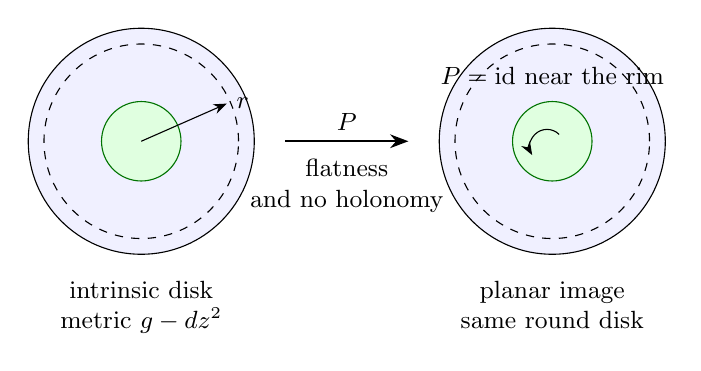
\begin{tikzpicture}[scale=.87,>=Stealth,font=\small]
\begin{scope}
\filldraw[fill=blue!6,draw=black] (0,0) circle (1.65);
\filldraw[fill=green!12,draw=green!45!black] (0,0) circle (.58);
\draw[dashed] (0,0) circle (1.42);
\draw[->] (0,0)--(1.25,.55) node[right] {$r$};
\node[below,align=center] at (0,-1.9) {intrinsic disk\\metric $g-dz^2$};
\end{scope}
\draw[->,thick] (2.1,0)--(3.9,0) node[midway,above] {$P$};
\node[align=center] at (3,-.65) {flatness\\and no holonomy};
\begin{scope}[xshift=6cm]
\filldraw[fill=blue!6,draw=black] (0,0) circle (1.65);
\filldraw[fill=green!12,draw=green!45!black] (0,0) circle (.58);
\draw[dashed] (0,0) circle (1.42);
\draw[->] (.1,.1) arc[start angle=45,end angle=210,radius=.25];
\node at (0,.95) {$P=\id$ near the rim};
\node[below,align=center] at (0,-1.9) {planar image\\same round disk};
\end{scope}
\end{tikzpicture}
\caption{The inner fill removes the annular holonomy. Normalization
fixes the outer collar; half-turn symmetry fixes the center of the
inner disk. Properness then upgrades the local development to a
global diffeomorphism. The sketch records these constraints, not
the pointwise distortion of $P$.}
\label{fig:development}
\end{figure}

\subsection{A stationary cap which distinguishes shapes}

We need more than a cap that closes the graph. A completely symmetric
cap could hide the relative rotation. The following explicit marker
reduces the possible congruences to a finite set.

\begin{lemma}\label{lem:fixed-cap}
A smooth graph over $D_{r_+}$ which is horizontal near its boundary
extends to a smooth embedded sphere. The complementary cap may be
chosen to contain the unique global maximum of Gaussian curvature,
with distinct principal curvatures at that point.
\end{lemma}

\begin{proof}
Translate the boundary height to zero and extend the horizontal
collar to a radius $R>r_+$. Choose a smooth nondecreasing function
$\chi:[0,1]\to[0,1]$, constant at its endpoint values near the
endpoints and satisfying $\chi(1-t)=1-\chi(t)$. The unit-speed
meridian starting at $(R,0)$ with
\[
 r'(s)=\cos(\pi\chi(s/L)),\qquad
 z'(s)=-\sin(\pi\chi(s/L)),\qquad 0\le s\le L,
\]
stays at radius at least $R$ and returns to radius $R$ with inward
horizontal tangent. Its height decreases by a positive constant
times $L$. Take $L$ large enough to pass below the minimum of the
graph, and finish with a horizontal disk to the axis. Rotation of
this meridian gives a smooth embedded cap disjoint from the graph
except at its attaching collar.

Place a bump in the unused horizontal annulus $r_+<r<R$. In local
Cartesian coordinates choose $A,B>0$ with $A\ne B$, put
$\xi=Ax^2+By^2$, and set
\[
 u(x,y)=\frac{k}{2}\int_\xi^{\rho^2}
       e^{-s/(\rho^2-s)}\,ds\quad(\xi<\rho^2),
 \qquad u=0\quad(\xi\ge\rho^2).
\]
This is smooth across its support boundary. If
$\Xi=\xi/(\rho^2-\xi)$, the curvature of its graph is
\begin{equation}\label{eq:marker-curvature}
 K=\frac{ABk^2e^{-2\Xi}(1-2\xi\Xi')}
 {\bigl[1+k^2e^{-2\Xi}(A^2x^2+B^2y^2)\bigr]^2}.
\end{equation}
At the center it equals $ABk^2$. Elsewhere its numerator is either
nonpositive or strictly smaller, and its denominator is at least
one. Choose $k$ to make this value larger than the curvature of the
rest of the sphere. Then choose $\rho$ small enough to fit the
support and keep its height, at most $k\rho^2/2$, away from the
bottom cap. The principal curvatures at the center are $-kA,-kB$
for the upward normal, so they are distinct.
\end{proof}

\begin{figure}[htbp]
\centering
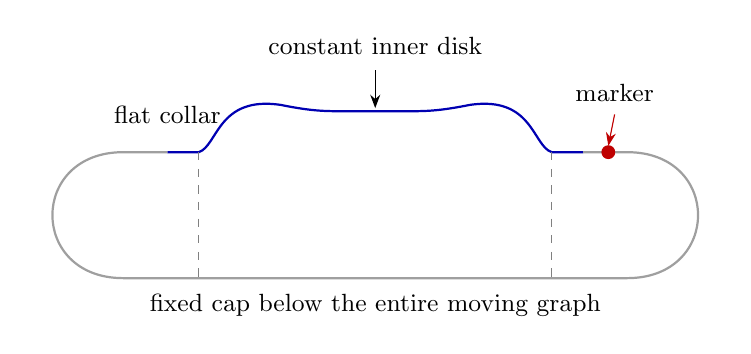
\begin{tikzpicture}[x=.8cm,y=.8cm,>=Stealth,font=\small]
\draw[thick,blue!70!black]
 (-3.3,0)--(-2.8,0) .. controls (-2.5,.1) and (-2.5,.9) .. (-1.5,.75)
 .. controls (-1,.65) and (-.8,.65) .. (-.5,.65)--(.5,.65)
 .. controls (.8,.65) and (1,.65) .. (1.5,.75)
 .. controls (2.5,.9) and (2.5,.1) .. (2.8,0)--(3.3,0);
\draw[thick,gray!75] (3.3,0)--(4,0)
 .. controls (5.5,0) and (5.5,-2) .. (4,-2)--(-4,-2)
 .. controls (-5.5,-2) and (-5.5,0) .. (-4,0)--(-3.3,0);
\fill[red!75!black] (3.7,0) circle (2.5pt);
\draw[dashed,gray] (-2.8,0)--(-2.8,-2);
\draw[dashed,gray] (2.8,0)--(2.8,-2);
\node[above] at (0,1.4) {constant inner disk};
\draw[->] (0,1.3)--(0,.7);
\node[above] at (-3.3,.3) {flat collar};
\node[above] at (3.8,.65) {marker};
\draw[->,red!75!black] (3.8,.6)--(3.7,.1);
\node[below] at (0,-2.1) {fixed cap below the entire moving graph};
\end{tikzpicture}
\caption{A meridional sketch of the closure. The actual blue graph
depends on angle; its whole rotation stays inside the central
cylinder and above the bottom disk. The marker lies in the
stationary horizontal extension.}
\label{fig:geometric-closure}
\end{figure}

\subsection{The annulus implies the theorem}

\begin{theorem}[Geometric closure]\label{thm:geometric-closure}
If a nonradial, half-turn invariant height $z$ for
\eqref{eq:intro-metric} is constant on two collars where $w=0$, and
$g-dz^2$ is positive and flat, then all the conclusions of
Theorem~\ref{thm:main} hold.
\end{theorem}

\begin{proof}
Develop the filled disk by Proposition~\ref{lem:disk-development}
and attach the cap of Lemma~\ref{lem:fixed-cap}. On the disk set
$F_\tau=R_{-2\pi\tau}\circ F\circ R_{2\pi\tau}$, and leave the
cap fixed. The intrinsic rotation preserves $g$. On the inner disk
and outer collar its action cancels the ambient rotation, since
$P$ is a centered rotation there and $z$ is constant. The formula
therefore glues smoothly in both variables and is one-periodic.
Each disk image is a rotation of a graph over the same round disk;
the separated cap closes it without introducing intersections.

The disk images cannot all coincide. Otherwise
$F^{-1}R_\vartheta F$ would be an intrinsic isometry equal to
$R_\vartheta$ on the outer collar. An isometry of a connected
Riemannian manifold is determined by its value and derivative at an
interior point, by geodesic uniqueness. Thus it would equal
$R_\vartheta$ everywhere. Its height component would force
$z(r,\theta+\vartheta)=z(r,\theta)$ for every $\vartheta$, contrary
to nonradiality.

Any congruence between two closed images fixes the unique curvature
maximum in the cap. It preserves the outward normal and the two
distinct principal lines there. There are at most four orthogonal
maps with these properties. If all the closed images were congruent,
their continuous family would therefore lie in a finite set and
would be constant. Its disk portion would be constant too, which
we have just excluded.

Finally, the moving disk is an ambient rotation of itself, while
the rest of the surface is stationary. This proves invariance of
area and of the oriented mean-curvature integral. If $Z_\tau$ is
the height over the planar disk and $c_B$ is the bottom height, the
part of the enclosed volume inside its cylinder is
\[
 \int_{D_{r_+}}(Z_\tau(y)-c_B)\,dy
 =\int_{D_{r_+}}(Z_0(R_{2\pi\tau}y)-c_B)\,dy,
\]
which is constant by rotation invariance of planar area. The
remaining volume is stationary.
\end{proof}

The task left for the analysis is now precise: construct one
nonradial annular height with a positive flat remainder metric and
constant endpoint extensions. The family itself then follows
without an additional existence argument.

\section{What the height equation requires}
\label{sec:scalar-core}

The geometric reduction leaves considerable freedom: we may choose
the rotational metric as well as its nonradial height. This section
identifies the conditions that guide those choices. A connection
form gives the scalar equation and its conservation law; its
linearization reveals the changes of type; a finite model then
separates the two resonance problems that the construction must solve.

\subsection{A curvature residual with a symmetric derivative}

Write $h'=w$, $E=1+w^2$, and introduce the local height jets
\begin{equation}\label{eq:height-jet-notation}
 k=z_r,\qquad p=z_\theta/r,\qquad
 D=E(1-p^2)-k^2,\qquad Q=k+Ep_\theta.
\end{equation}
The metric $g-dz^2$ is positive if and only if $D>0$. A useful
orthonormal coframe for it is
\[
 \eta_1=\frac{\sqrt D}{\sqrt{1-p^2}}\,dr,\qquad
 \eta_2=r\sqrt{1-p^2}\,d\theta-
             \frac{kp}{\sqrt{1-p^2}}\,dr.
\]
In this polar frame the Euclidean connection is $d\theta$.
We use $dr\,d\theta$ for all scalar adjoints; the source measure
must remain explicit when coordinates are changed later.

\begin{proposition}\label{prop:scalar-core}
For $D>0$, the connection form and the curvature residual are
\begin{align}
 \alpha&=D^{-1/2}\left(d\theta+\frac{k}{1-p^2}\,dp\right),
       \label{eq:conn-one-form}\\
 r\mathcal N_h(z)&=D^{-3/2}
 \left[Qk_r-Erp_r^2-\frac{E'}2(1-p^2+kp_\theta)\right],
       \label{eq:cart-curvature-scalar}
\end{align}
where $\mathcal N_h(z)=-\sqrt D\,K(g-dz^2)$ and
$d\alpha=r\mathcal N_h(z)\,dr\wedge d\theta$.
Holding $w$ fixed, the derivative is
\begin{equation}\label{eq:cart-true-derivative}
 rD_z\mathcal N_h(z)\eta
  =\partial_r(a\eta_r+b\eta_\theta)
       +\partial_\theta(b\eta_r+c\eta_\theta),
\end{equation}
with
\begin{equation}\label{eq:linear-coefficients}
 a=QD^{-3/2},\quad b=-Ep_rD^{-3/2},\quad
 c=r^{-1}(Ek_r-E'k/2)D^{-3/2}.
\end{equation}
Its determinant satisfies
\begin{equation}\label{eq:cart-determinant-identity}
 ac-b^2=\frac{K_0}{D^2}+ED^{-3/2}\mathcal N_h(z),
 \qquad K_0=\frac{ww'}r.
\end{equation}
\end{proposition}

\begin{proof}
Equality of mixed height derivatives gives
\begin{equation}\label{eq:height-compatibility}
 rp_r=k_\theta-p.
\end{equation}
Substitution in the two structure equations for $\eta_1,\eta_2$
gives \eqref{eq:conn-one-form}. Here is a direct check of its
curvature numerator, which also fixes all signs. Use
$D_r=E'(1-p^2)-2Epp_r-2kk_r$ and
$D_\theta=-2Epp_\theta-2kk_\theta$. The coefficient of
$dr\wedge d\theta$ in $D^{3/2}d\alpha$ is
\[
 -\tfrac12D_r+\frac{D}{1-p^2}(k_rp_\theta-k_\theta p_r)
 -\frac{k}{2(1-p^2)}(D_rp_\theta-D_\theta p_r).
\]
Replacing $k_\theta-p$ by $rp_r$ reduces it to the bracket in
\eqref{eq:cart-curvature-scalar}. This is also the Darboux numerator:
\begin{equation}\label{eq:darboux-numerator}
 Qk_r-Erp_r^2-\frac{E'}2(1-p^2+kp_\theta)=0.
\end{equation}
For example the Christoffel symbols are
$\Gamma^r_{rr}=E'/2E$, $\Gamma^r_{\theta\theta}=-r/E$,
$\Gamma^\theta_{r\theta}=1/r$, and
\begin{equation}\label{eq:radial-curvature}
 K_g=E'/(2rE^2).
\end{equation}
These formulas give the same numerator from
\eqref{eq:intro-darboux}.

For the variation, set $B_1=k/((1-p^2)\sqrt D)$. The identities
$(B_1)_k=ED^{-3/2}$ and $(B_1)_E=-k/(2D^{3/2})$ give
\begin{equation}\label{eq:conn-exact-variation}
 \delta\alpha=d(B_1\delta p)
  +(a\eta_r+b\eta_\theta)\,d\theta
  -(b\eta_r+c\eta_\theta)\,dr,
 \qquad\delta p=\eta_\theta/r.
\end{equation}
Taking the exterior derivative removes the exact term and proves
\eqref{eq:cart-true-derivative}. In particular the normal flux is
$a\eta_r+b\eta_\theta$.

Finally, let $N$ denote the bracket in
\eqref{eq:cart-curvature-scalar}. Since
$kQ+D=E(1-p^2+kp_\theta)$,
\[
 ac-b^2=\frac E{rD^3}\left(N+\frac{E'D}{2E}\right).
\]
Using $N=rD^{3/2}\mathcal N_h(z)$ proves the determinant identity.
\end{proof}

At the radial height $z=h$, these expressions simplify to
$D=1$, $a=w$, $b=0$, $c=w'/r$. Thus
\begin{equation}\label{eq:intro-linearization}
 \mathscr L_wu=(wu_r)_r+\frac{w'}r u_{\theta\theta}.
\end{equation}
For $w>0$ it is elliptic where $w'>0$ and hyperbolic where $w'<0$.
A simple zero of $w'$ is a turning circle. Notice that it is the
slope of the profile that changes sign, not the profile itself.

\subsection{Why the endpoint must keep changing type}

It is tempting to take an uncomplicated bump for $w$, solve in its
middle, and flatten its ends. The next observation explains why
that does not preserve a nonzero infinitesimal height.

\begin{proposition}[The monotone-end obstruction]
\label{prop:obs-monotone-tail}
Let $w>0$ on $(r_-,r_+)$ be $C^1$, with $w(r_-)=0$ and $w'\ge0$
near $r_-$. If a continuous endpoint extension of a solution satisfies
\[
 (wf')'-j^2w'f/r=0,\qquad f(r_-)=0,\qquad
 \lim_{r\downarrow r_-}wf'=0,
\]
then $f=0$. The analogous assertion holds at a right endpoint with
$w(r_+)=0$ and $w'\le0$ nearby.
\end{proposition}

\begin{proof}
Integrating the flux equation and putting
$m(r)=\max_{r_-\le t\le r}|f(t)|$ gives
\[
 |f'(r)|\le \frac{j^2}{w(r)}
       \int_{r_-}^r\frac{w'(t)}t|f(t)|\,dt
 \le\frac{j^2}{r_-}m(r).
\]
Integration once more and Gronwall's inequality give $m=0$ on a
collar; ordinary interior uniqueness continues the zero. At the
right endpoint integrate backwards and use
$\int_r^{r_+}|w'|=w(r)$. The proof also applies to complex $f$.
\end{proof}

Consequently a positive profile with only finitely many changes of
monotonicity cannot carry our endpoint-flat nonzero angular mode.
The infinitely many turning circles are forced by this obstruction
within the present construction. Their amplitudes and widths will
decrease fast enough that the profile nevertheless extends smoothly.

\begin{figure}[htbp]
\centering
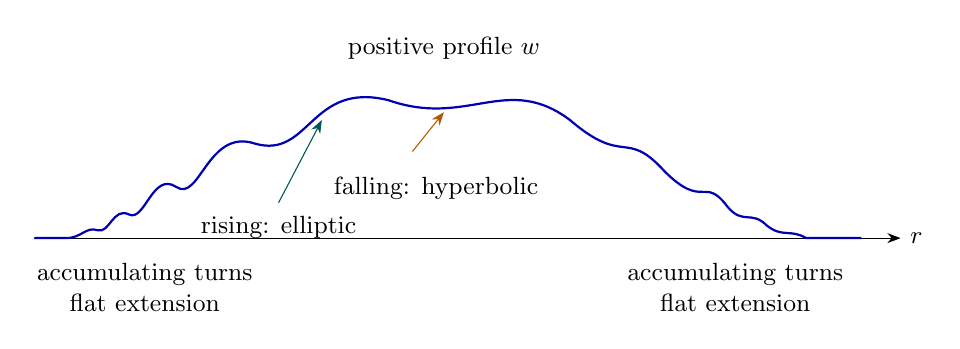
\begin{tikzpicture}[x=1cm,y=1cm,>=Stealth,font=\small]
\draw[->] (0,0)--(11,0) node[right] {$r$};
\draw[thick,blue!70!black] (0,0)--(.4,0)
 .. controls (.6,0) and (.65,.15) .. (.8,.1)
 .. controls (.95,.05) and (1,.4) .. (1.2,.3)
 .. controls (1.4,.2) and (1.5,.85) .. (1.8,.65)
 .. controls (2.1,.45) and (2.2,1.4) .. (2.8,1.2)
 .. controls (3.5,1) and (3.5,2) .. (4.5,1.75)
 .. controls (5.5,1.4) and (6,2.1) .. (6.8,1.5)
 .. controls (7.5,.9) and (7.5,1.4) .. (8.0,.85)
 .. controls (8.5,.35) and (8.5,.8) .. (8.8,.4)
 .. controls (9.0,.16) and (9.1,.36) .. (9.3,.16)
 .. controls (9.5,0) and (9.6,.12) .. (9.8,0)--(10.5,0);
\node[above] at (5.2,2.15) {positive profile $w$};
\node[below,align=center] at (1.4,-.2) {accumulating turns\\flat extension};
\node[below,align=center] at (8.9,-.2) {accumulating turns\\flat extension};
\draw[->,orange!70!black] (4.8,1.1)--(5.2,1.6);
\node[below] at (5.1,.9) {falling: hyperbolic};
\draw[->,teal!70!black] (3.1,.45)--(3.65,1.5);
\node[below] at (3.1,.4) {rising: elliptic};
\end{tikzpicture}
\caption{Why there are infinitely many interfaces. The drawing shows
only finitely many representative turns, without their actual scales.
On each rising interval the linearized equation is elliptic; on each
falling interval it is hyperbolic. Every derivative still tends to
zero at the accumulation endpoints.}
\label{fig:profile-type}
\end{figure}

\subsection{Two denominators in one finite model}
\label{sec:worked-example}

The next calculation is a guide to the spectral construction, not
an approximation to its full inverse. Set $\epsilon=\sqrt2/100$,
$\rho(X)=\epsilon^2X(1-X)$, and on $[-1,2]$ solve
\begin{equation}\label{eq:example-radius}
 r_{XX}=-\rho r,\qquad r(0)=1,\qquad r_X(0)=1/10.
\end{equation}
Its integral equation bounds $R:=\max|r|$ by
$R\le1.2+8\epsilon^2R$, so $R<1.203$,
$r>0.798$, and $|r_X-.1|\le4\epsilon^2R<.001$.
Hence $w(r(X))=r_X(X)$ is a genuine positive radial profile.
It has two simple turning points, at $X=0,1$.
For an angular mode $j$ and $J=j\epsilon$, its equation becomes
\begin{equation}\label{eq:example-mode}
 L_jU=\frac1{r_X}\bigl(U_{XX}+J^2X(1-X)U\bigr).
\end{equation}

The characteristics have slopes
$d\theta/dX=\pm\epsilon\sqrt{X(1-X)}$ on $0<X<1$.
Their travel angle is
\begin{equation}\label{eq:example-action}
 T=\epsilon\int_0^1\sqrt{X(1-X)}\,dX=\epsilon\pi/8.
\end{equation}
The difference of the two endpoint translations acts by
\begin{equation}\label{eq:example-circle-operator}
 \mathcal D_T f=f(\theta+T)-f(\theta-T),\qquad
 \mathcal D_T\sin(j\theta)=2\sin(jT)\cos(j\theta).
\end{equation}
Thus straightening the two characteristic returns costs the divisor
$\sin(jT)$. For this quadratic irrational travel angle the integer
$2j^2-640000m^2\ne0$, where $m$ is nearest to $j\sqrt2/800$, yields
\begin{equation}\label{eq:example-diophantine-bound}
 |\sin(jT)|\ge (320000j)^{-1}.
\end{equation}
Indeed factor that integer, use
$j\sqrt2/800+|m|\le j$, and then
$|\sin(\pi x)|\ge2\dist(x,\mathbb Z)$.
The inverse of $\mathcal D_T$ therefore loses one angular derivative.

Now impose a radial boundary condition. Under
$x=\sqrt J(X-1/2)$ the homogeneous equation becomes
\begin{equation}\label{eq:example-oscillator}
 (-\partial_x^2+x^2)U=(J/4)U.
\end{equation}
At each end of the finite interval take the solution line obtained
by restricting the corresponding decaying solution of this
whole-line oscillator. These are legitimate boundary lines for
\eqref{eq:example-mode}; the radius itself need not extend outside
$[-1,2]$. The two lines agree exactly at an oscillator eigenvalue.
Since those eigenvalues are $2m+1$
\cite[Section~8.3]{Teschl2009}, the resonance is
\begin{equation}\label{eq:example-spectral-phase}
 J/4=2m+1,
 \qquad\text{or equivalently}\qquad
 jT=(m+\tfrac12)\pi.
\end{equation}
For an inhomogeneous source, multiply by $-r_X/J$, extend by zero
outside $[-3\sqrt J/2,3\sqrt J/2]$, apply the whole-line oscillator
resolvent, and restrict back. This proves that the prescribed boundary
problem has precisely these spectral denominators; it is not just
a comparison of formal phases.

\begin{figure}[htbp]
\centering
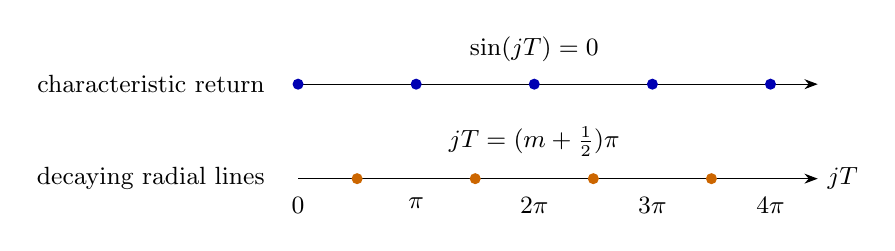
\begin{tikzpicture}[x=1.5cm,y=.8cm,>=Stealth,font=\small]
\node[anchor=east] at (-.2,1.5) {characteristic return};
\node[anchor=east] at (-.2,0) {decaying radial lines};
\draw[->] (0,1.5)--(4.4,1.5);
\draw[->] (0,0)--(4.4,0) node[right] {$jT$};
\foreach \x/\t in {0/0,1/\pi,2/2\pi,3/3\pi,4/4\pi}{
 \fill[blue!70!black] (\x,1.5) circle (2pt);
 \node[below] at (\x,-.15) {$\t$};}
\foreach \x in {.5,1.5,2.5,3.5}{
 \fill[orange!80!black] (\x,0) circle (2pt);}
\node[above] at (2,1.7) {$\sin(jT)=0$};
\node[above] at (2,.2) {$jT=(m+\tfrac12)\pi$};
\end{tikzpicture}
\caption{Two distinct resonance sets in the exact finite model.
The horizontal variable is the phase, with marks spaced by $\pi$.
Controlling one row does not control the other. Both must stay
separated when the cells of the infinite construction are joined.}
\label{fig:two-denominators}
\end{figure}

The half-step shift also has a local interpretation. Near $X=0$,
put $y=J^{2/3}X$. Then
\[
 U_{yy}+yU=J^{-2/3}y^2U.
\]
On any fixed $y$-interval the leading solutions are
$\operatorname{Ai}(-y),\operatorname{Bi}(-y)$, with an error
$O(J^{-2/3})$ in value and first derivative for fixed initial data.
Variation of constants against their bounded fundamental matrix
on that interval, followed by Gronwall, gives this estimate.
Their standard asymptotics carry the phase shift $\pi/4$ at each
turn \cite[9.7.5--9.7.12]{DLMFAiry}. The exact oscillator calculation,
rather than this local heuristic, proves
\eqref{eq:example-spectral-phase}.

\subsection{Normalization, conservation and the first residual correction}

The nonlinear unknown is $z=h+qu$. Divide its residual by the small
parameter, using the removable definition
\begin{equation}\label{eq:cart-removable-equation}
 \mathcal A=\mathcal F_q(w,u)=
 \begin{cases}r\mathcal N_h(h+qu)/q,&q\ne0,\\
 \mathscr L_wu,&q=0.
 \end{cases}
\end{equation}
Smoothness at zero follows from the exact formula
\begin{equation}\label{eq:normalized-integral}
 \mathcal F_q(w,u)=\int_0^1 rD_z\mathcal N_h(h+tqu)u\,dt.
\end{equation}
We work with heights even in $\theta$ and invariant under
$\theta\mapsto\theta+\pi$. Nonlinear products preserve this class.
For functions constant at the endpoint collars, Stokes' theorem
applied to the connection gives
\begin{equation}\label{eq:zero-total-integral}
 \int_{r_-}^{r_+}\av{\mathcal F_q(w,u)}\,dr=0,
 \qquad \av f=\frac1{2\pi}\int_0^{2\pi}f\,d\theta.
\end{equation}
Both boundary periods equal $2\pi$. Every differential of this
identity, including metric differentials, has the same compatibility.
Constants in $u$ do not affect the equation.
\label{lem:scalar-integral}

The mean is more transparent at the level of the connection period.
For $U=z-h$ set
\begin{equation}\label{eq:cart-mean-path-flux}
 \mathfrak F_w(U)=\av{\alpha_\theta}-1
 =\left\langle\frac{1+kp_\theta/(1-p^2)}{\sqrt D}\right\rangle-1.
\end{equation}
Its derivative is $r\av{\mathcal N_h(h+U)}$, and its endpoint
value is zero. If $U=Z+m(r)$ with $\av Z=0$, the mean equation
is therefore $\mathfrak F_w(Z+m)=0$. Formula
\eqref{eq:conn-exact-variation} gives
\begin{equation}\label{eq:mean-period-derivative}
 \partial_{m'}\mathfrak F_w(U)=\av a,
 \qquad D_U\mathfrak F_w(0)[U]=w\av{U_r}.
\end{equation}
This linear cancellation is the reason the mean can later gain
twice the decay of the nonconstant height.

The true linearization has one inconvenient feature: away from a
solution, the residual term in
\eqref{eq:cart-determinant-identity} moves the turning circles.
We remove that term while preserving the normal flux.

\begin{lemma}[Fixing the type-change set]\label{lem:type-completion}
On the neighborhood $D\ge1/2$, $Q\ge7w/8>0$, put
\[
 B=E/(rQ),\qquad \bar c=c-Br\mathcal N_h(z),\qquad
 \bar L=\partial_r(a\partial_r+b\partial_\theta)
             +\partial_\theta(b\partial_r+\bar c\partial_\theta).
\]
Then
\begin{equation}\label{eq:cart-completed-normalized-derivative}
 a\bar c-b^2=K_0/D^2,\qquad
 D_u\mathcal F_q\eta=\bar L\eta+
                 q\partial_\theta(B\mathcal A\eta_\theta).
\end{equation}
The corrected operator is symmetric for $dr\,d\theta$, kills
constants, and has the same normal flux as the true derivative.
\end{lemma}

\begin{proof}
The change in determinant is
$aBr\mathcal N_h=ED^{-3/2}\mathcal N_h$, exactly the unwanted
term. The change of operator is
$\partial_\theta(Br\mathcal N_h\partial_\theta)$;
substitute $r\mathcal N_h=q\mathcal A$.
Only the tangential coefficient changed, proving the remaining
assertions.
\end{proof}

The correction vanishes with the equation being solved. Its error
is bilinear in the residual and the increment, the form needed in
Hamilton's implicit theorem. A second correction will fix the
characteristic returns. For reference the present characteristic
slopes on a negative component are
\begin{equation}\label{eq:completed-characteristics}
 \frac{d\theta}{dr}=d\pm v_{\mathrm{char}},\qquad
 d=\frac{E(p-k_\theta)}{rQ},\qquad
 v_{\mathrm{char}}=\frac{\sqrt{-ww'/r}\sqrt D}{Q}.
\end{equation}
At a simple turning circle this speed is a smooth positive factor
times the square root of inward distance. The subsequent coordinate
construction must respect that degeneracy; merely treating all
intervals as uniformly elliptic would lose the geometry of the problem.

\section{Designing a profile with one surviving angular mode}
\label{sec:rosen-reference-packet}
\label{sec:radial-models}

The geometric construction asks for a nonradial height which becomes
exactly constant at two ends.  Its first-order version already tells us
what the radial metric must do.  For
\[
 u(r,\theta)=u_0(r)+\sum_{\substack{j\ge2\\j\ {
m even}}}u_j(r)e_j(\theta),
 \qquad e_j(\theta)=\sqrt2\cos(j\theta),
\]
the linearized equation is a family of ordinary differential equations:
\begin{equation}\label{eq:rad-eq-modal-operator}
 L_ju=(wu')'-j^2\frac{w'}r u,
 \qquad
 \mathscr L_wu=(wu_r)_r+\frac{w'}r u_{\theta\theta}.
\end{equation}
We want exactly one endpoint-flat solution among the nonzero angular
modes.  We choose its frequency to be two, the first frequency compatible
with the half-turn symmetry used in the geometric closure.  The
nonlinear equation will create the higher even frequencies, so they
must all have inverses on this same profile.

There are two freedoms here.  The shape of a local profile determines
its oscillation and its spectrum.  Multiplying that profile by a positive
constant changes its flux scale without changing its homogeneous
solutions.  We use the first freedom to obtain explicit local models,
and the second to prevent a resonance when neighboring models are
joined.  This separation is the organizing idea of the construction.

\subsection{What the radial construction must supply}

We record the analytic interface before choosing the models.  The estimates
are stated in the original radius, so no change of source measure is
implicit.  Angular brackets denote normalized angular average.

\begin{definition}[The three endpoint scales]\label{def:radial-weights}
The cells approaching either endpoint are indexed by $n\ge N$.  Set
\begin{equation}\label{eq:rad-eq-endpoint-weights}
 A_n\asymp e^{-n^2},\qquad
 S_n=\frac23 n^3,\quad H_n=e^{-S_n},\qquad
 q_n=n^{5/2}\log(e+n),\quad \mathcal E_n=e^{q_n}.
\end{equation}
A coefficient estimate of order $s$ on cell $n$ means an estimate by
$C_s\mathcal E_n^{C_s}$.  The same notation on the finitely many central
pieces denotes fixed positive constants.  A cell includes fixed portions
of its neighboring positive intervals; a bounded enlargement changes
its index by at most a fixed integer.
\end{definition}

The length scale $A_n$ measures how much room is available.  The much
smaller quantity $H_n$ will measure the decay of the distinguished
solution.  The intermediate weight $\mathcal E_n$ pays for taking
reciprocals and derivatives of the coefficients.  Section~\ref{sec:radial-tails}
derives all three scales from a continuous construction; they are not
independent hypotheses about an unknown profile.

Choose a smooth partition $\vartheta_m$ with bounded overlap on the
cells and the finite middle; $m$ records both the endpoint and the cell
index.  For fixed $0<\gamma<1$, write
\begin{equation}\label{eq:rad-eq-source-norm}
 \|(f,c)\|_{Y_{\gamma,s}}^2
 =|c|^2+\sum_m\mathcal E_m^{2M_0}H_m^{-2\gamma}
       \|\vartheta_m f\|_{L^2(dr)H^s(\T)}^2.
\end{equation}
The output norm at angular order zero replaces
$\mathcal E_m^{2M_0}$ by $\mathcal E_m^{-2M_1}$.
In that norm the zero mode is written $a_L\chi_L+v_0$, where
$\chi_L$ is a fixed smooth function equal to one near the left endpoint
and zero near the right.  We include $|a_L|$ and the scalar unknown
below in the output norm.

\begin{proposition}[The fixed radial reference]\label{prop:rad-fixed-theorem}
There is a positive smooth profile $w_*$ on a finite interval
$(r_-,r_+)$, flat at both endpoints, with only simple interior zeros of
$w_*'$.  It has the following properties.

There is a nonzero endpoint-flat function $\phi_*$ with
$L_2\phi_*=0$.  This is the whole endpoint-flat kernel at frequency two;
the kernel is zero at every even frequency $j\ge4$.  Every component
of $\{w_*'<0\}$ has travel angle $T_m$ satisfying
\begin{equation}\label{eq:rad-eq-optical-margin}
 |\sin(kT_m)|\ge\gamma_m/|k|\quad(k\ge1),
 \qquad \gamma_m^{-1}\le\mathcal E_m^{C},
 \qquad T_m/\pi\text{ is quadratic irrational}.
\end{equation}
There is a smooth $\chi_*$ supported in a positive component such that
\begin{equation}\label{eq:rad-eq-target-border}
 g_*=L'_{2,w_*}[w_*\chi_*]\phi_*,\qquad
 \int g_*\phi_*\,dr=1,\qquad
 \ell_*u=\int g_*u_2\,dr.
\end{equation}
The bordered operator
\begin{equation}\label{eq:rad-eq-bordered-reference}
 \mathbb L_{w_*}(u,\nu)
   =\bigl(\mathscr L_{w_*}u+\nu g_*e_2,\ell_*u\bigr)
\end{equation}
has a two-sided inverse on compatible sources,
$\int\langle f\rangle\,dr=0$, with right endpoint height zero and
one free left endpoint constant.  For every compact interval
$[\gamma_-,\gamma_+]\Subset(0,1)$ there are fixed $M_0,M_1$ for which
this inverse is bounded from $Y_{\gamma,0}$ to the output norm above,
uniformly for $\gamma$ in that interval.  One radial derivative costs
at most one additional angular derivative of the source.  The profile,
its kernel and the border are the same for all these exponents.
\end{proposition}

Here $L'_{2,w}[v]\phi=(v\phi')'-4v'\phi/r$ is the derivative
with respect to the radial profile; the source is still a density in $dr$.
The proof occupies this section and the next two.  Its conclusion is a
base inverse estimate, including the endpoint realization.  Higher total
orders will be recovered from the differential equation after the
weighted spaces have been introduced.  Keeping these two tasks separate
avoids making the choice of geometry depend on the eventual regularity
order.

\subsection{Turning a spectral potential into a radial metric}

It is easier to design the spectrum before designing the radius.  Let
$X$ be a model coordinate, let $r_X=v>0$, and choose a positive density
$\mathcal P$.  Put
\begin{equation}\label{eq:rad-eq-sc0}
 \begin{gathered}
 w(r(X))=\lambda\mathcal P(X)v(X),\qquad
 \rho=-\frac{r_{XX}+(\mathcal P_X/\mathcal P)r_X}{r},\qquad
 V_0=\frac{(\sqrt{\mathcal P})_{XX}}{\sqrt{\mathcal P}},\\
 L_j(\mathcal P^{-1/2}\psi)
   =-\frac{\lambda\sqrt{\mathcal P}}{v}
      \bigl(-\psi_{XX}+(V_0-j^2\rho)\psi\bigr).
 \end{gathered}
\end{equation}
Indeed $wu_r=\lambda\mathcal P u_X$, and differentiating this expression
and using the definition of $\rho$ gives the identity.  Thus a
Schr\"odinger model determines the radial equation once its radius
satisfies the displayed linear equation and remains increasing.
The factor $\lambda$ is absent from the homogeneous model.

Our two choices have complementary jobs.  The central oscillator
retains the desired zero mode.  The Morse models near the ends have
explicit nonzero gaps, but are short enough in radius to accumulate
at a finite point.  Figure~\ref{fig:two-spectral-models} illustrates the
potentials; it is their solvable spectra, rather than the qualitative
shapes alone, that make them useful.

\begin{figure}[htbp]
\centering
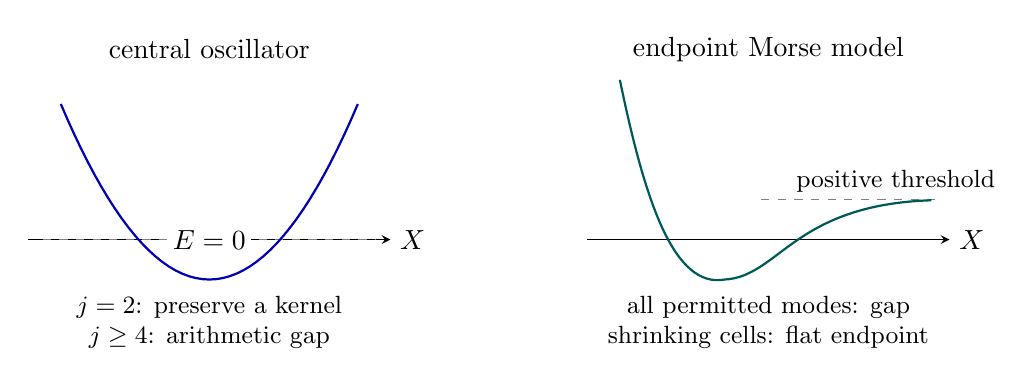
\begin{tikzpicture}[x=.92cm,y=.78cm,>=stealth]
\begin{scope}
\draw[->] (-2.5,0)--(2.5,0) node[right] {$X$};
\draw[dashed,gray] (-2.3,0)--(2.3,0);
\draw[thick,blue!70!black,domain=-2.05:2.05,samples=45]
 plot (\x,{.68*\x*\x-.65});
\node[align=center] at (0,3.1) {central oscillator};
\node[fill=white,inner sep=2pt] at (0,0) {$E=0$};
\node[align=center,font=\small] at (0,-1.35)
 {$j=2$: preserve a kernel\\$j\ge4$: arithmetic gap};
\end{scope}
\begin{scope}[xshift=7.1cm]
\draw[->] (-2.5,0)--(2.5,0) node[right] {$X$};
\draw[dashed,gray] (-.1,.65)--(2.3,.65);
\draw[thick,teal!70!black]
 (-2.05,2.6) .. controls (-1.7,.6) and (-1.3,-.8) .. (-.6,-.65)
 .. controls (.15,-.6) and (.35,.57) .. (2.25,.64);
\node[align=center] at (0,3.1) {endpoint Morse model};
\node[anchor=west,font=\small] at (.25,.95) {positive threshold};
\node[align=center,font=\small] at (0,-1.35)
 {all permitted modes: gap\\shrinking cells: flat endpoint};
\end{scope}
\end{tikzpicture}
\caption{The two full-line spectral models, drawn schematically with an
arbitrary vertical scale.  Only finite pieces are used in the surface.
Positive end regions separate those pieces when they are joined.}
\label{fig:two-spectral-models}
\end{figure}

\subsection{The central oscillator}
\label{subsec:rad-central-singlepoint}

Set
\begin{equation}\label{eq:rad-eq-sc1}
 A_c=1/\sqrt2,\qquad a_c=\sqrt{4A_c-2},\qquad
 c_c=3A_c-2>0,\qquad \alpha_c=(c_c+1)/2.
\end{equation}
Take $\mathcal P=e^{-2a_cX}$ and $\rho=A_c-X^2$.
Then the model operator is
\[
 H_{j,c}=-\partial_X^2+j^2X^2+a_c^2-j^2A_c.
\]
Its standard oscillator spectrum is
\begin{equation}\label{eq:central-spectrum-new}
 E_{m,j}=j(2m+1)+a_c^2-j^2A_c,\qquad m=0,1,\ldots;
\end{equation}
see \cite[\S8.3, equations (8.33)--(8.42)]{Teschl2009}.
The choice of $a_c$ sets $E_{0,2}=0$.  The irrational choice of $A_c$
keeps the other even frequencies away from zero.

Here is the quantitative part of that last assertion.  Put
$\Phi_j=jA_c-a_c^2/j$.  For even $j\ge4$,
\[
 N_j:=j^2/2-\Phi_j^2=2A_ca_c^2-a_c^4/j^2
\]
lies between $13/4-3\sqrt2/2$ and $4-2\sqrt2$, so its distance
from the integers is at least
$\delta=\tfrac34(3-2\sqrt2)>0$.
If $|E_{m,j}|<1$, then $2m+1=\Phi_j+E_{m,j}/j$ and
$2m+1+\Phi_j<2j$.  Since $j^2/2-(2m+1)^2$ is an integer,
\[
 \delta\le |(2m+1)^2-\Phi_j^2|<2|E_{m,j}|.
\]
This also yields the bound when $|E_{m,j}|\ge1$.  At $j=2$ the levels
are $4m$.  Consequently
\begin{equation}\label{eq:rad-eq-sc3}
 \|H_{j,c}^{-1}\|\le2/\delta\quad(j\ge4\text{ even}),
 \qquad \ker H_{2,c}=\operatorname{span}\{e^{-X^2}\},
\end{equation}
and the reduced inverse at $j=2$ has norm $1/4$.
We use the closed quadratic-form realization in these statements.

We still need an increasing radius; an arbitrary solution of the radius
equation would not suffice.  An explicit positive one is
\begin{equation}\label{eq:rad-eq-sc6}
 \psi_1(X)=e^{-X^2/2}\int_0^\infty
 t^{\alpha_c-1}e^{-t^2/2+\sqrt2Xt}\,dt,
 \qquad r=e^{a_cX}\psi_1,\qquad \upsilon=r_X/r.
\end{equation}
An integration by parts in $t$ shows that
$\psi_1''=(X^2+c_c)\psi_1$.
The function is positive, while $\psi_1,\psi_1'$ tend to zero as
$X\to-\infty$.  Hence $\psi_1''>0$ implies $\psi_1'>0$ and
$\upsilon=a_c+\psi_1'/\psi_1>a_c$.  Using
$c_c-a_c^2+A_c=0$ gives
$r_{XX}-2a_cr_X+(A_c-X^2)r=0$, exactly the equation in
\eqref{eq:rad-eq-sc0}.  In particular this spectral model really is a
radial metric.

For later cuts, the needed end estimates are
\begin{equation}\label{eq:rad-eq-sc6a}
 \upsilon=
 \begin{cases}
 -X+a_c-\alpha_c/X+O(X^{-3}),&X\to-\infty,\\
 X+a_c+(\alpha_c-1)/X+O(X^{-3}),&X\to+\infty.
 \end{cases}
\end{equation}
These estimates hold after any fixed number of derivatives.  For
$X=-L$, substitute $t=z/(\sqrt2L)$ in the integral; the remaining
integral is $\Gamma(\alpha_c)(1+O(L^{-2}))$ and can be differentiated
under its exponentially integrable majorant.  For $X>0$, complete the
square and expand $t^{\alpha_c-1}$ about $\sqrt2X$ against the Gaussian;
the part $|t-\sqrt2X|>X/2$ is exponentially small.  Logarithmic
differentiation gives \eqref{eq:rad-eq-sc6a}.
Thus $r$ ranges from zero to infinity, and
$\upsilon\asymp1+|X|$.

The surviving radial height and its logarithmic slope are
\begin{equation}\label{eq:rad-eq-sc2}
 \phi_0=e^{a_cX-X^2},\qquad
 \frac{\partial_y\phi_0}{\phi_0}=\frac{a_c-2X}{\upsilon}
       \longrightarrow 2\ \text{on the left},\quad -2\ \text{on the right},
 \qquad y=\log r.
\end{equation}
Writing $w=re^f$, the radius equation also gives
\begin{equation}\label{eq:rad-eq-sc6b}
 1+f_y=\frac{X^2-A_c}{\upsilon^2}\longrightarrow1.
\end{equation}
We may therefore cut far enough out that both end regions are positive
and have uniformly bounded logarithmic-coordinate jets.  There are
just two simple turning points in the retained middle.  Its travel angle
is $\pi A_c/2=\pi/(2\sqrt2)$, whose sine divisors satisfy
$|\sin(kT)|\ge c/k$ by the integer norm $|k^2-8m^2|\ge1$.

There is one measure conversion worth settling now.  Define
\begin{equation}\label{eq:rad-eq-ha2}
 \varpi=12w/r^2,\quad B_j=-\varpi^{-1}L_j,
 \qquad
 \|u\|_{L^2(\varpi dr)}^2=12\lambda\|\upsilon\psi\|_2^2,
 \quad u=\mathcal P^{-1/2}\psi.
\end{equation}
The inverse in this measure contains
$\upsilon H_{j,c}^{-1}\upsilon$, not merely $H_{j,c}^{-1}$.
It is uniformly bounded.  Indeed
$V_j\ge c j^2\upsilon^2-Cj^2$ and the spectral gap first give
$\|\upsilon H_{j,c}^{-1}\|\le C$; taking adjoints gives the bound
on the other side.  For $\psi=H_{j,c}^{-1}(\upsilon F)$,
\[
 cj^2\|\upsilon\psi\|_2^2
 \le \|\upsilon\psi\|_2\|F\|_2+Cj^2\|F\|_2^2,
\]
and absorption yields the two-sided weight bound.  At $j=2$, add the
projection onto $e^{-X^2}$, apply the same argument, and subtract that
projection.  Its weighted norm is finite.

We will temporarily border mode two by a compact function $g_0$ with
$\int g_0\phi_0\,dr=1$ and row $\ell_0u=\int g_0u\,dr$.
The source obstruction is removed by pairing with $\phi_0$; adding a
multiple of $\phi_0$ fixes the row.  Thus this bordered inverse has the
same bounds.  Normalize its Hilbert scalar so that under a height
rescaling $w\mapsto\lambda w$ one has
$g_0\mapsto\sqrt\lambda g_0$, $\phi_0\mapsto\phi_0/\sqrt\lambda$.
Both the row and column then have bounded Hilbert norm.  This is an
auxiliary border, changed to \eqref{eq:rad-eq-target-border} after all
geometric choices have been made.

\subsection{Morse models: two quantitative gaps from one irrationality}

For the tails take $\mathcal P=1$ and
\[
 \rho(X)=A(e^{-X}-e^{-2X})-B,
 \qquad H_{j,M}=-\partial_X^2-j^2\rho,
 \qquad A>4B>0.
\]
The essential spectrum starts at $j^2B$; below it the simple eigenvalues
are
\begin{equation}\label{eq:rad-eq-fs1}
 E_{m,j}=j^2B-(\alpha_j-m)^2,
 \qquad \alpha_j=(j\sqrt A-1)/2,\qquad 0\le m<\alpha_j.
\end{equation}
This is the Morse spectrum \cite{Morse1929}.  For completeness, the
factorization which fixes its normalization is short.  With
$\omega=j\sqrt A$ and $D_\alpha=\partial_X+\alpha-\omega e^{-X}$,
\[
 H_\alpha=D_\alpha^*D_\alpha+j^2B-\alpha^2,
 \qquad
 H_{\alpha-1}=D_\alpha D_\alpha^*+j^2B-\alpha^2.
\]
The null function of $D_\alpha$ is
$e^{-\alpha X-\omega e^{-X}}$, square integrable exactly for
$\alpha>0$.  Descending by integers removes one ground state at a
time.  At $-1<\alpha\le0$,
$H_\alpha-j^2B=D_0^*D_0-2\omega\alpha e^{-X}\ge0$;
there are no further levels.  Reversing the intertwining recovers every
level in \eqref{eq:rad-eq-fs1}.  The quadratic-form realization justifies
these identities by cutoff integration.  At the left end the potential
is confining, and at the right it approaches $j^2B$ exponentially;
the usual compact-perturbation argument gives the stated essential
threshold \cite[Theorem~6.19]{Teschl2009}.  These facts suffice for the
resolvent estimates below, all at energy zero.

Choose a nonsquare integer $d$ and set
\begin{equation}\label{eq:rad-eq-rm5}
 A=(d^{-1/2}+2d^{-9/2})^2,
 \qquad B=d^{-9}.
\end{equation}
For positive integers $j$ and odd $M$,
\[
 |j/\sqrt d-M|\ge (4j\sqrt d)^{-1}.
\]
If the difference is smaller than $1/2$, this follows by factoring the
nonzero integer $j^2-dM^2$; otherwise it is immediate.  At a discrete
level write $\kappa=(j\sqrt A-M)/2>0$.  Since
$\sqrt A-2\sqrt B=d^{-1/2}$,
\[
 |j^2B-\kappa^2|
 \ge \frac{j\sqrt B}{2}|j/\sqrt d-M|
 \ge\frac1{8d^5}.
\]
Together with the threshold $j^2d^{-9}$ this proves
\begin{equation}\label{eq:rad-eq-rm1}
 \|H_{j,M}^{-1}\|\le8d^9\qquad(j\ge2).
\end{equation}

The same irrationality controls the characteristic return.  The change
$t=e^{-X}$ gives
\begin{equation}\label{eq:rad-eq-rm2}
 T=\int_{\rho>0}\sqrt\rho\,dX
   =\pi(\sqrt A/2-\sqrt B)=\frac\pi{2\sqrt d}.
\end{equation}
To evaluate the integral, write the positive quadratic as
$A(t-t_-)(t_+-t)$ and use $t=c+h\cos\xi$; the elementary integral is
$\pi(c-\sqrt{c^2-h^2})$.  Here $t_-+t_+=1$ and
$t_-t_+=B/A$.  Factoring the integer $k^2-4dm^2$, with $m$ the nearest
integer to $k/(2\sqrt d)$, yields
\begin{equation}\label{eq:rad-eq-morse-small-divisor}
 |\sin(kT)|\ge(3k\sqrt d)^{-1}\qquad(k\ge1).
\end{equation}
For $k<\sqrt d$ use $m=0$ directly; otherwise the factorization gives
distance at least $(6k\sqrt d)^{-1}$ from the integers.
Thus one parameter choice supplies both local spectral separation and
return-angle separation.  They remain distinct conditions when the
models are joined: a junction can create a new spectral resonance
without changing any individual travel angle.  The next section deals
with that remaining freedom.

\section{Reaching a flat endpoint with an infinite chain}
\label{sec:radial-tails}
\label{sec:radial-selection}

A finite collection of turning circles cannot produce the endpoint
behavior we need.  The construction instead repeats a small local
mechanism infinitely often.  On one part of each cell the solution has
almost constant value and its flux changes; on the next part its flux
is almost constant and its value changes.  The exact continuous equation
then has a discrete recurrence with a large diagonal.  Its decaying
solution loses approximately $e^{-2n^2}$ on crossing cell $n$.
Accumulating those losses gives $e^{-2n^3/3}$, fast enough to survive
every fixed number of derivatives in the shrinking radial intervals.

This section makes that picture precise.  We first build the actual
smooth profile, then derive the recurrence without discarding its error
terms.  Only after those estimates are established do we choose the
height ratios which prevent matching resonances.

\subsection{The budget of lengths, amplitudes and errors}

Let $d_n$ be the least nonsquare integer not smaller than $e^{n^2}$.
Then $d_n=e^{n^2}+O(1)$.  Use \eqref{eq:rad-eq-rm5} with this integer,
writing the resulting parameters $A_n$ and $B_n$; thus
$A_n\asymp e^{-n^2}$ and $B_n\asymp A_n^9$.
Initially let $\lambda_n=e^{-n^{5/2}}$.  Later we allow
\begin{equation}\label{eq:rad-eq-js2}
 \lambda_n=e^{-n^{5/2}}\prod_{k=N}^n\sigma_k,
 \qquad 1\le\sigma_k\le2.
\end{equation}
Their logarithms change by at most $O(n)$, which does not disturb the
scale comparisons below.

The choices can be understood before the details of the profile are
computed.  A finite-order derivative on a cell of size $e^{-n^2}$
costs $e^{C_sn^2}$.  Its amplitude must decay faster; the exponent
$n^{5/2}$ does this.  The solution itself must decay faster still in
order to pay for inverse coefficients.  Its cubic exponent will come
from the recurrence.  These requirements leave the interval
$2<5/2<3$, rather than singling out an optimal numerical exponent.

\begin{table}[htbp]
\centering
\begin{tabularx}{\linewidth}{@{}l l X@{}}
\toprule
Quantity & Size & Purpose\\
\midrule
Radial cell length & $A_n\asymp e^{-n^2}$ & Summable lengths at a finite endpoint.\\
Profile amplitude & $e^{-n^{5/2}+O(n)}$ & Flatness after every fixed derivative cost $e^{C_sn^2}$.\\
Positive joining length & $\asymp A_n^{12}$ & A large height change has negligible transfer error.\\
Allowed matching angle & $\delta_n=c_0e^{-n^2}$ & Summable bad sets over all frequency bands.\\
Solution attenuation & $e^{-S_n}$, $S_n=2n^3/3$ & Integrability and flat extension of the selected solution.\\
Coefficient allowance & $\mathcal E_n=e^{n^{5/2}\log(e+n)}$ & Absorbs fixed coefficient and coordinate losses while remaining smaller than $e^{\varepsilon S_n}$.\\
\bottomrule
\end{tabularx}
\caption{The scale choices are a budget for distinct jobs.  Their
compatibility is verified in the construction and recurrence below.}
\label{tab:endpoint-budget}
\end{table}

In particular, for fixed $a,b,\varepsilon>0$,
\begin{equation}\label{eq:rad-scale-separation}
 \mathcal E_n^a e^{bn^2}\le C_{a,b,\varepsilon}e^{\varepsilon S_n},
 \qquad n^2=o(q_n),\qquad q_n=o(S_n).
\end{equation}
These comparisons concern fixed derivative orders.  No assertion of
uniform bounds as the derivative order tends to infinity is being made.

\subsection{A cell of the actual radial profile}

On a Morse interval solve
\begin{equation}\label{eq:rad-eq-rm4}
 r_X=v>0,\qquad v_X=-\rho r,\qquad
 \rho=A(e^{-X}-e^{-2X})-B,\qquad w=\lambda v.
\end{equation}
The last identity in \eqref{eq:rad-eq-sc0} becomes
$L_j=-(\lambda/v)H_{j,M}$.  Let $X_R$ be the right zero of $\rho$.
Prescribe $r(X_R)=1$, $v(X_R)=\delta A^5$ with fixed small
$\delta>0$.  Retain the model from $X_c=-\log(3/2)$ to
$X_R+c_RA^{-4}$, for a fixed sufficiently small $c_R>0$.

Here are the estimates which ensure this is a genuine increasing
radius.  On $[X_c,X_R]$ the weighted integral of $|\rho|$ is $O(A)$,
so the reverse Volterra equation
\[
 r(X)=1-v(X_R)(X_R-X)
       -\int_X^{X_R}(Y-X)\rho(Y)r(Y)\,dY
\]
gives $r=1+O(A)$.  At the left cut it yields
\begin{equation}\label{eq:rad-eq-rm6a}
 v(X_c)=3A/8+O(A^2),\qquad
 r(X_c)=1-15A/16+O(A^2).
\end{equation}
The two leading integrals, after $t=e^{-X}$, are
$\int_0^{3/2}(1-t)\,dt=3/8$ and
$\int_0^{3/2}\log((3/2)/t)(1-t)\,dt=15/16$.
The constant $B$ contributes only $O(B\log^2(A/B))=o(A^2)$.
On the negative component, backward integration from $X_R$ keeps
$v$ positive; on the short left positive component its minimum is the
positive value at $X_c$.  On the long right positive component,
comparison with $r_{XX}=Br$ gives
\begin{equation}\label{eq:rad-eq-rm6}
 \begin{gathered}
 r=1+O(A),\qquad cA^5\le v\le CA,\qquad
 v\asymp A^5\text{ on the long right part},\\
 \Delta r\asymp A,\qquad
 \int_{X_c}^{X_R}v^2\,dX\asymp A^2,\qquad
 \int_{\text{each positive cap}}\sqrt{-\rho}\,dX\asymp\sqrt A.
 \end{gathered}
\end{equation}
For the last long-cap estimate use
$\sqrt B\,A^{-4}\asymp\sqrt A$; on the short cap
$-\rho\ge cA$ on a fixed subinterval.  Taking $c_R$ small ensures
that $r$ stays in a fixed positive range throughout this argument.

Multiply $r,v$ by a radius factor $\mathfrak r_n$.  To pass from a
cell to its next neighbor in the increasing-$r$ direction, insert a
positive interval of length
\begin{equation}\label{eq:rad-eq-rm7}
 \ell_{n,m}=c_Cr_o\min(A_n,A_m)^{12},\qquad m=n\pm1,
\end{equation}
where $r_o$ is its initial radius.  Choose the neighboring radius
factor so that its left endpoint is $r_o+\ell_{n,m}$.
The ratio of successive radius factors is $1+O(A_n+A_m)$.
The recursion converges on either end, with a prescribed limiting
radius on the left.  Thus the radii stay in a compact subset of
$(0,\infty)$ and all cells accumulate at finite endpoints.

At this joining interval the profile increases from $W_L$ to $W_R$,
with
\begin{equation}\label{eq:height-contrast-new}
 \log(W_R/W_L)=4n^2+O(n^{3/2}+n).
\end{equation}
To match the complete smooth germs, put $f=\log w$ and prescribe
\begin{equation}\label{eq:rad-eq-rm8}
 f'=\chi_Lf_L'+\chi_Rf_R'+C_1(1-\chi_L-\chi_R),
 \qquad
 C_1=\frac{\log(W_R/W_L)-\int\chi_Lf_L'-\int\chi_Rf_R'}
             {\int(1-\chi_L-\chi_R)}.
\end{equation}
The end cutoffs have disjoint supports and equal one near the respective
ends.  Their derivative integrals are
$O(\ell_{n,m}/\min(A_n,A_m))$, whereas the required logarithmic
height change is comparable to $n^2$.  Hence $C_1>0$ and, after the
fixed initial index is increased, $w'/w\ge2/r$ on the joining interval.
Integrating $f'$ with the left value matches the right value and all
endpoint derivatives.

This explains the apparently extravagant exponent $12$.
The height contrast costs $e^{4n^2+o(n^2)}$.  At the largest frequency
assigned to this cell, $j^2$ costs $e^{n^2}$ times a polynomial.
The interval length contributes $e^{-12n^2+o(n^2)}$.
Their product is $e^{-7n^2+o(n^2)}$, much smaller than the allowed
matching angle $e^{-n^2}$.  The same choice makes both the mass and
resistance of the join negligible in the estimates below.  No minimal
choice of this exponent is needed.

\paragraph{Flatness and coefficient bounds.}
The length of cell $n$ is comparable to $A_n$, and
$A_{n+1}/A_n=e^{-2n-1}(1+o(1))$.  If $d_\partial$ is distance to the
endpoint, then on that cell and its assigned joins
\begin{equation}\label{eq:geometry-endpoint-distance}
 cA_{n+1}\le d_\partial\le CA_n,
 \qquad \log(d_0/d_\partial)=n^2+O(n).
\end{equation}
All interval lengths and their reciprocals are bounded by $e^{Cn^2}$.
On a model, $\partial_r=v^{-1}\partial_X$ and $v\ge c\mathfrak r_nA_n^5$.
The differential equations for $r,v$ bound every fixed derivative of
$\log v$ by $e^{C_sn^2}$.  Formula~\eqref{eq:rad-eq-rm8} gives the
same bound on the joins.  Since each derivative of $e^{\pm\log w}$
contains only one undifferentiated exponential, we obtain
\begin{equation}\label{eq:geometry-profile-jets}
 \begin{gathered}
 e^{-n^{5/2}-Cn^2}\le w\le e^{-n^{5/2}+Cn^2},\\
 |\partial_r^sw|\le C_se^{-n^{5/2}+C_sn^2},\qquad
 |\partial_r^s(w^{-1})|\le C_se^{n^{5/2}+C_sn^2}.
 \end{gathered}
\end{equation}
Comparison with \eqref{eq:geometry-endpoint-distance} proves that
extension by zero is smooth and flat.  It also proves the fixed-order
coefficient bounds in Definition~\ref{def:radial-weights}, uniformly in
all height choices \eqref{eq:rad-eq-js2}.

\subsection{Why a mass--resistance chain appears}

Use $y=\log r$.  For the mode-two comparison density
$\mathsf p=wr^7$, divide a cell into a mass interval $I_n$ (the short
positive cap and the negative component) and a resistance interval
$J_n$ (the long positive cap and its following short join).  Define
\begin{equation}\label{eq:mass-resistance-def-new}
 \mu_n=\int_{I_n}\mathsf p\,dy,\quad
 R_n^I=\int_{I_n}\mathsf p^{-1}\,dy,\quad
 \nu_n=\int_{J_n}\mathsf p\,dy,\quad
 R_n=\int_{J_n}\mathsf p^{-1}\,dy.
\end{equation}
For an equation $-(\mathsf p V_y)_y=\Lambda\mathsf p V$, the change
of flux across an almost constant-value region is its value times
$-\Lambda$ times the mass.  The change of value across an almost
constant-flux region is the flux times the resistance.  This gives the
picture in Figure~\ref{fig:mass-resistance-chain}; the estimates following
it turn the picture into an exact reduction.

\begin{figure}[htbp]
\centering
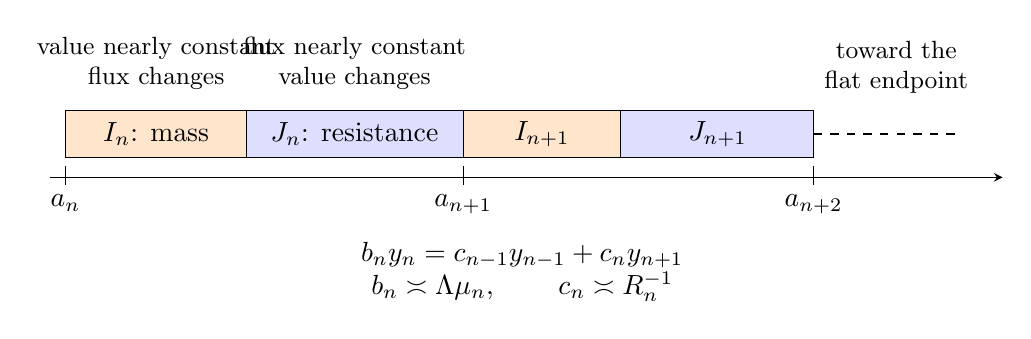
\begin{tikzpicture}[x=1cm,y=1cm,>=stealth]
\draw[->] (0,0)--(12.1,0);
\node[align=center,font=\small] at (10.75,1.4)
 {toward the\\flat endpoint};
\draw[fill=orange!20] (.2,.25) rectangle (2.5,.85);
\draw[fill=blue!13] (2.5,.25) rectangle (5.25,.85);
\draw[fill=orange!20] (5.25,.25) rectangle (7.25,.85);
\draw[fill=blue!13] (7.25,.25) rectangle (9.7,.85);
\draw[dashed] (9.7,.55)--(11.5,.55);
\node at (1.35,.55) {$I_n$: mass};
\node at (3.87,.55) {$J_n$: resistance};
\node at (6.25,.55) {$I_{n+1}$};
\node at (8.48,.55) {$J_{n+1}$};
\foreach \x/\lab in {.2/a_n,5.25/a_{n+1},9.7/a_{n+2}}
 {\draw (\x,-.1)--(\x,.15);\node[below] at (\x,-.1) {$\lab$};}
\node[align=center,font=\small] at (1.35,1.45) {value nearly constant\\flux changes};
\node[align=center,font=\small] at (3.87,1.45) {flux nearly constant\\value changes};
\node[align=center] at (6,-1.2)
 {$b_n y_n=c_{n-1}y_{n-1}+c_ny_{n+1}$\\
 $b_n\asymp\Lambda\mu_n$, \qquad $c_n\asymp R_n^{-1}$};
\end{tikzpicture}
\caption{The continuous intervals and their exact node equation.
The drawing is schematic; $a_n=(-1)^ny_n$ for the decaying solution.
Large products $\Lambda\mu_nR_n$ make successive node values small.}
\label{fig:mass-resistance-chain}
\end{figure}

Since $dr=v\,dX$, the two measures in
\eqref{eq:mass-resistance-def-new} are $wr^6dr$ and $dr/(wr^8)$.
Using \eqref{eq:rad-eq-rm6} gives
\begin{equation}\label{eq:rad-eq-rm10}
 \mu_n\asymp\lambda_nA_n^2,\qquad
 R_n^I\le C\lambda_n^{-1}\log(A_n/B_n),\qquad
 \nu_n\le C\lambda_nA_n^6,\qquad
 R_n\asymp\lambda_n^{-1}A_n^{-4}.
\end{equation}
A radius dilation multiplies the mass by its eighth power and the
resistance by its inverse eighth power; the products below are unchanged.
The joining interval contributes at most $W_R\ell$ to mass and
$\ell/W_L$ to resistance.  Their relative errors are respectively
$e^{-7n^2+O(n^{3/2}+n)}$ and $e^{-11n^2+O(n)}$, so
\begin{equation}\label{eq:rad-eq-rm11}
 \mu_nR_n\asymp A_n^{-2},\qquad
 \mu_nR_n^I\le CA_n^2\log(A_n/B_n),\qquad
 \nu_nR_n\le CA_n^2,
\end{equation}
while
\begin{equation}\label{eq:rad-eq-rm12}
 \log(\mu_{n+1}R_n)=2n^2+O(n^{3/2}+n).
\end{equation}

The same structure handles a general frequency.  The exact gauge
$u=r^{j^2}V$ gives
\begin{equation}\label{eq:rad-eq-rm13}
 (\mathsf p_jV_y)_y+\Lambda\mathsf p_jV=0,
 \qquad \mathsf p_j=wr^{2j^2-1},\qquad \Lambda=j^2(j^2-1).
\end{equation}
After removing its constant endpoint factor,
$\mathsf p_j/\mathsf p=(r/r_\partial)^{2(j^2-4)}$.
On the tail beyond $N$ its logarithm is bounded by $Cj^2A_N$.
Thus the mass and resistance comparisons remain uniform whenever
$j^2A_N$ is bounded.  The stronger condition used below is
\begin{equation}\label{eq:deep-frequency-condition-new}
 j^2A_N\sqrt{\log(A_N/B_N)}\le c.
\end{equation}

\subsection{The exact continuous-to-discrete reduction}

Orient $x=\log r$ on the right and $x=-\log r$ on the left, so $x$
always increases toward the flat endpoint.  On the left the outward
order is $J_N,I_N,J_{N+1},I_{N+1},\ldots$; therefore, within this
reduction only, the resistance following $I_n$ is the original
$J_{n+1}$.  This one-index change affects only the lower-order terms
in \eqref{eq:rad-eq-rm12}.  The initial $J_N$ is treated as a separate
resistance edge.

The following conditions isolate precisely what is needed from the
profile.  For a positive density $\mathsf p$, assume
\begin{equation}\label{eq:rad-eq-dg1}
 \begin{gathered}
 \Lambda\mu_nR_n^I+\Lambda\nu_nR_n\le\eta\ll1,\qquad
 \Lambda\mu_nR_n,\ \Lambda\mu_{n+1}R_n\ge K\gg1,\\
 \nu_n\le\eta\min(\mu_n,\mu_{n+1}).
 \end{gathered}
\end{equation}
An initial resistance edge has the same large-product conditions and
$\Lambda\nu_0R_0\le\eta$, $\nu_0\le\eta\mu_N$.
Call this a \emph{deep tail}.  Equations
\eqref{eq:rad-eq-rm10}--\eqref{eq:deep-frequency-condition-new} imply
these conditions for $\mathsf p_j$ after the initial index is large
enough.

\begin{lemma}[Deep inverse and unique decaying line]
\label{lem:radial-deep-inverse}
\label{lem:radial-flat-line}
On a deep tail let
$A_{\mathsf p}=-\mathsf p^{-1}(\mathsf p\partial_x)'$ act in
$\mathcal H=L^2(\mathsf p\,dx)$, with Dirichlet condition at the finite
entrance and the Friedrichs condition at the outer endpoint.  Then
\[
 \|(A_{\mathsf p}-\Lambda)^{-1}\|\le C/\Lambda.
\]
The homogeneous equation has exactly one square-integrable line at
the outer endpoint.  At successive mass entrances its nonzero values
are $a_n=(-1)^ny_n$, with $y_n>0$ and
\begin{equation}\label{eq:rad-eq-dg4}
 \frac{y_{n+1}}{y_n}
 =\frac{1+O(\eta)+O(K^{-1})}{\Lambda\mu_{n+1}R_n},
 \qquad
 \frac{\sqrt{\mu_{n+1}}y_{n+1}}{\sqrt{\mu_n}y_n}\le C/K<1/2.
\end{equation}
For the constructed Morse tails this line, transferred back to $u$,
is smooth and flat in the original radius.
\end{lemma}

\begin{proof}
We give the reduction on the continuous equation, so that the endpoint
condition and the operator norm follow from the same argument.
Introduce resistance coordinate $ds=dx/\mathsf p$ on an edge
$E_n=I_n\cup J_n$.  Its length is $L_n=R_n^I+R_n$ and its density is
$\omega=\mathsf p^2$, so $\mathsf p\,dx=\omega\,ds$ and
\[
 (A_{\mathsf p}-\Lambda)u=f
 \quad\Longleftrightarrow\quad -u_{ss}-\Lambda\omega u=\omega f.
\]
The zero-potential Dirichlet kernel is
$G_0(s,t)=\min(s,t)[L_n-\max(s,t)]/L_n$.
The small quantity in this equation is
\[
 \delta_n^{\rm edge}=\Lambda\int\omega(s)G_0(s,s)\,ds\le3\eta,
 \qquad R_n^I/L_n\le\eta/K.
\]
The kernel inequality
$G_0(s,z)G_0(z,t)\le G_0(s,t)G_0(z,z)$ bounds its resolvent series
term by term.  Hence the actual kernel and the two boundary-height
functions satisfy
\begin{equation}\label{eq:rad-eq-dg2}
 G_0\le G_\Lambda\le(1-\delta_n^{\rm edge})^{-1}G_0,
 \qquad l_i\le v_i\le(1-\delta_n^{\rm edge})^{-1}l_i,
 \quad l_0=1-s/L_n, l_1=s/L_n.
\end{equation}
The analogous inequality for the Poisson functions follows by replacing
one kernel factor by $l_i$.  For a zero-boundary $u$,
$\Lambda\int\omega|u|^2\le\delta_n^{\rm edge}\int|u_s|^2$.
Thus the direct sum $G_D$ of the Dirichlet edge inverses has norm
at most $C\eta/\Lambda$.

The outward derivative matrix of this exact edge problem is
\[
 \begin{pmatrix}d_{n,0}&-c_n\\-c_n&d_{n,1}\end{pmatrix},\qquad
 c_n=L_n^{-1}+\Lambda\int\omega l_0v_1,\qquad
 d_{n,i}=L_n^{-1}-\Lambda\int\omega l_iv_i.
\]
Since $l_0l_1=G_0(s,s)/L_n$, we have
\begin{equation}\label{eq:rad-eq-dg3}
 c_n=R_n^{-1}(1+O(\eta)),\qquad
 b_n:=-d_{n-1,1}-d_{n,0}
       =\Lambda\mu_n(1+O(\eta)+O(K^{-1})).
\end{equation}
For the second estimate, the mass on $I_n$ sees
$l_0=1+O(R_n^I/L_n)$.  The preceding edge contributes at most
$\nu_{n-1}+\mu_{n-1}(R_{n-1}^I/L_{n-1})^2$; the second term is
at most $\eta^2K^{-2}\mu_n$ by \eqref{eq:rad-eq-dg1}.
The two $L^{-1}$ terms are at most $2\Lambda\mu_n/K$.
These calculations also cover the initial resistance edge.

For node values $a=(a_n)$ put
$(Ta)|_{E_n}=a_nv_0+a_{n+1}v_1$ and let
$\mathfrak h=\ell^2(\mu_n)$.  Equation~\eqref{eq:rad-eq-dg2} gives
\begin{equation}\label{eq:rad-eq-dj1}
 c\|a\|_{\mathfrak h}^2\le\|Ta\|_{\mathcal H}^2
                         \le C\|a\|_{\mathfrak h}^2.
\end{equation}
For example, on $I_n$ the squared neighbor term costs at most
$C\mu_n(R_n^I/L_n)^2|a_{n+1}|^2$; after an index shift its sum is
$O(\eta^2/K^2)\|a\|_{\mathfrak h}^2$.  The mass of $J_n$ is handled
by its last inequality in \eqref{eq:rad-eq-dg1}.

The shifted quadratic form on these interpolants is
\[
 (\mathcal Da,a)_{\mathfrak h}
   =-\sum b_n|a_n|^2-2\operatorname{Re}\sum c_na_n\overline{a_{n+1}}.
\]
In coordinates $\sqrt{\mu_n}a_n$, the diagonal has size $\Lambda$,
while each of the two neighboring entries is bounded by
$C/(R_n\sqrt{\mu_n\mu_{n+1}})\le C\Lambda/K$.
Diagonal dominance therefore gives
$\|\mathcal D^{-1}\|\le C/\Lambda$, independently of the number
of edges.

These algebraic formulas give an operator inverse because they respect
the form domain.  The interpolation energy is bounded by
$C\Lambda\|a\|_{\mathfrak h}^2$ using its shifted form and
\eqref{eq:rad-eq-dj1}.  Conversely, averaging $u(x_n)-u(x)$ on
$I_n$ gives
\[
 \mu_n|u(x_n)|^2\le2\|u\|_{I_n}^2+
             2\mu_nR_n^I\int_{I_n}|u_s|^2.
\]
Thus every form-domain function has square-summable node data and
splits as $Ta+v$, where $v$ vanishes at every node.  The two parts
are orthogonal for the shifted form, by the homogeneous edge equation.
Consequently the exact inverse is
\begin{equation}\label{eq:rad-eq-dj2}
 (A_{\mathsf p}-\Lambda)^{-1}=G_D+T\mathcal D^{-1}T^*,
 \qquad (T^*f)_n=\mu_n^{-1}\int\mathsf p\,(T\mathbf e_n)f\,dx.
\end{equation}
Finite Dirichlet truncations have this same formula and converge
strongly: the uniformly convergent diagonal resolvent series for
$\mathcal D^{-1}$ converges on finite compressions, and the direct edge
terms do as well.  Their limit is the Friedrichs realization just
identified by the form decomposition.  This proves the inverse bound.

For the homogeneous line, substituting $a_n=(-1)^ny_n$ gives
$b_ny_n=c_{n-1}y_{n-1}+c_ny_{n+1}$.
Set $\epsilon_n=c_n^2/(b_nb_{n+1})\le C/K^2$ and
$t_n=b_{n+1}y_{n+1}/(c_ny_n)$.  Backward elimination is
\[
 t_n=(1-\epsilon_{n+1}t_{n+1})^{-1}.
\]
For large $K$ these maps preserve $[1,2]$ and contract by at most
$1/2$.  Finite outer walls therefore give a unique bounded limiting
sequence.  Equation~\eqref{eq:rad-eq-dg3} yields
\eqref{eq:rad-eq-dg4}, and \eqref{eq:rad-eq-dj1} makes its
interpolation square integrable.
An independent node solution has the Wronskian form
\[
 z_n=y_n\left(C+\mathcal W\sum_{k=N}^{n-1}
                \frac1{c_ky_ky_{k+1}}\right),\qquad\mathcal W\ne0.
\]
Successive summands grow by at least $cK^2$, so eventually
$|z_{n+1}/z_n|\asymp\Lambda\mu_nR_n$ and
$\sqrt{\mu_{n+1}}|z_{n+1}|\ge cK\sqrt{\mu_n}|z_n|$.
On the mass interval its neighbor term is at most $C\eta$ times its
own-node term.  Its continuous $L^2$ mass therefore diverges.
This proves uniqueness of the square-integrable line and the
limit-point property.

Finally, summing \eqref{eq:rad-eq-rm12} in
\eqref{eq:rad-eq-dg4} gives, for $k\ge m$,
\begin{equation}\label{eq:rad-eq-rm17}
 \left|\frac{a_k}{a_m}\right|
 \le\mathcal E_k^C\mathcal E_m^C e^{-(S_k-S_m)},\qquad
 2\sum_{n=m}^{k-1}n^2
 =\frac23(k^3-m^3)-(k^2-m^2)+\frac13(k-m).
\end{equation}
The accumulated $O(n^{3/2}+n)$ error is absorbed by $q_k+q_m$.
Every fixed radial derivative costs at most $e^{C_sn^2}$, by the
profile equation and the interval lengths.  The normalized gauge
$(r/r_\partial)^{j^2}$ is bounded with bounded inverse in the deep
range.  Thus the constructed homogeneous solution and all its fixed
radial derivatives are bounded by $\mathcal E_n^{C_s}e^{-S_n}$
after a fixed entrance normalization.  They extend flatly at the
endpoint.  The same contraction also shows continuity of the endpoint
line in the product topology of all the height ratios.
\end{proof}

\paragraph{The localized Green estimate.}
We will use a little more than the operator norm.  Let $B$ be the
positive node matrix with diagonal $b_n$ and neighboring entries
$-c_n$, and let $W=\operatorname{diag}(\mu_n)$.
Define
$\Gamma_{nm}=(\mu_n\mu_m)^{-1/2}
 (W^{-1/2}BW^{-1/2})^{-1}_{nm}$.
Its diagonal lies between $b_m^{-1}$ and $Cb_m^{-1}$ by the
positive diagonal series.  Uniqueness of the decaying recurrence gives
\begin{equation}\label{eq:rad-eq-dj4}
 \Gamma_{nm}=\Gamma_{mm}\frac{y_n}{y_m}
 \le\frac{C}{\Lambda\mu_m}
      \prod_{k=m}^{n-1}\frac{1+C(\eta+K^{-1})}{\Lambda\mu_{k+1}R_k}
 \quad(n\ge m).
\end{equation}
Symmetry handles the reverse direction.  The interpolation kernel in
\eqref{eq:rad-eq-dj2} has the additional sign $-(-1)^{n+m}$, which
is irrelevant to absolute estimates.  The continuous kernel adds the
same-edge Dirichlet term and at most two interpolation functions at
each endpoint.  Hence its localized absolute bound is
\begin{equation}\label{eq:rad-eq-dj5}
 C\mathcal E_n^C\mathcal E_m^C e^{-|S_n-S_m|}.
\end{equation}
For the original source convention, put
$g=(r/r_\partial)^{j^2}$ and $\mathsf p^\circ=g^2w/r$.
A direct calculation gives
\[
 L_j(gV)=-\frac{gw}{r^2}(A_{\mathsf p^\circ}-\Lambda)V,
 \qquad \mathsf p^\circ dx=\frac{g^2w}{r^2}\,dr,
 \qquad G_{L_j}(r,r')=-g(r)g(r')G_A(x,x').
\]
The bounded gauge factors preserve \eqref{eq:rad-eq-dj5} in the
$dr$ pairing.  Also, for $B_j=-\varpi^{-1}L_j$,
\begin{equation}\label{eq:rad-eq-rm20}
 B_j=\frac1{12}(A_{\mathsf p_j}-j^2(j^2-1)),
 \qquad \|B_{j,D}^{-1}\|\le Cj^{-4}
\end{equation}
on a deep tail.  At its entrance the derivative matrix gives
$\mathsf p u_x/(\Lambda\mu_nu)=1+O(\eta)+O(K^{-1})$.
If an initial resistance edge comes first, the impedance is instead
$-(1+O(\eta)+O(K^{-1}))/R_0$.  In either case the endpoint
Green pairing vanishes: at the nodes it is bounded by
$C\Lambda\mu_n|a_n|^2\to0$, and finite mass and energy identify this
with the endpoint limit.

\subsection{One transition cell at every frequency}

The useful decomposition depends on frequency, although the geometry
does not.  Put
\begin{equation}\label{eq:rad-eq-rm21}
 \mathcal H_n=C_*q_nA_n^{-1/2},\qquad
 \mathcal I_n=\{j:\mathcal H_{n-1}\le j<\mathcal H_n\}.
\end{equation}
At the initial index $N$, include every remaining even frequency
$2\le j<\mathcal H_N$ in the first band.  For $j\in\mathcal I_n$,
all earlier cells have large positive-cap action
$j\sqrt{A_m}\ge C_*q_m$.  Cell $n$ is the transition cell; the
next one is already deep, since
\begin{equation}\label{eq:rad-eq-rm22}
 j^2A_{n+1}\sqrt{\log(A_{n+1}/B_{n+1})}
 \le Cq_n^2(A_{n+1}/A_n)(n+1)\longrightarrow0.
\end{equation}
Thus there is no unexamined frequency range between the local model
inverse and the deep inverse.  This one-transition-cell decomposition
will be crucial when the inverse is assembled.

At each finite tail entrance attach an auxiliary positive cone $w=cr$.
For the right tail it continues to $r=0$, and for the left tail to
$r=\infty$.  A short positive interpolation with $rw'/w\ge1$ is
constructed by applying \eqref{eq:rad-eq-rm8} to $\log(w/r)$.
The cone merely specifies an incoming line.  The final surface retains
only a finite piece of it.  In $y=\log r$,
\[
 B_j=\tfrac1{12}(-\partial_y^2+j^2),\qquad
 \varpi\,dr=12c\,dy;
\]
the incoming lines are $r^j$ and $r^{-j}$ respectively, and the
Dirichlet inverse has norm at most $12/j^2$.

\subsection{Choosing the heights so that the lines do not meet}

For $j\in\mathcal I_n$, select the positive join immediately before
cell $n$ in the outward order.  Its inner height $W_{\rm in}$ does
not depend on $\sigma_n$, while its outer height is
$\sigma_nW_{\rm out}^0$.  Write
\begin{equation}\label{eq:rad-eq-js4}
 \Xi_n=W_{\rm out}^0/W_{\rm in},\qquad
 \Upsilon_n=\max(\Xi_n,\Xi_n^{-1}),\qquad
 \log\Upsilon_n=4n^2+O(n^{3/2}+n).
\end{equation}
The radius recursion and all cut locations are independent of the height
choices.  At the first join choose the auxiliary cone amplitude
independently of $\sigma_N$, with the same contrast as in
\eqref{eq:rad-eq-js4}.
All later pieces are multiplied by the same $\sigma_n$, so their
homogeneous equations, and hence their natural endpoint line, are
unchanged.  The incoming line is determined before this join and is
also independent of $\sigma_n$.  What changes is the flux scale by
which the two lines are compared.

We first control the incoming slope.  Set
\begin{equation}\label{eq:rad-eq-js5}
 \zeta_j=ru_r/j^2-u.
\end{equation}
The solution coming from a Dirichlet cut in the preceding positive cap
can be normalized to $u=1$ at the join, and then
\begin{equation}\label{eq:rad-eq-js6}
 a:=\zeta_j/u\in[-3/2,-1/2].
\end{equation}
Indeed on that cap $u_{XX}=j^2|\rho|u$.
Comparison of $u_X/u$ with the constant-potential Riccati solution
gives
$|u_X/u|\le Cj\sqrt b\coth(cj\sqrt A)$, where the cap scales are
$(b,h,v)\asymp(A,1,A)$ or $(A^9,A^{-4},A^5)$.
In both cases $h\sqrt b\asymp\sqrt A$ and
$v\asymp\sqrt{Ab}$, so
$|ru_r/(j^2u)|\le C/(j\sqrt{A_{n-1}})<1/2$ after choosing $C_*$
large.  Reversing the left orientation changes only the sign.
In the first band the cone gives $ru_r/(j^2u)=\pm1/j$, proving the
same assertion even at $j=2$.

The derivative $w'/w$ can be very large on the short join.  It disappears
from the transfer equation if we use the right state.  The identity
$(w\zeta_j)'=-(j^2-1)wu_r/j^2$ gives, for
$Y=(u,w\zeta_j/W_{\rm in})$,
\begin{equation}\label{eq:rad-eq-js7}
 Y_r=\frac1r
 \begin{pmatrix}
 j^2&j^2W_{\rm in}/w\\
 -(j^2-1)w/W_{\rm in}&-(j^2-1)
 \end{pmatrix}Y.
\end{equation}
The transfer therefore differs from the identity by at most
$e^{\eta_{n,j}}-1$, where
\begin{equation}\label{eq:rad-eq-js14}
 \eta_{n,j}=Cj^2(\ell_n/r_{\min})\Upsilon_n
 \le CC_*^2q_n^2e^{-7n^2+O(n^{3/2}+n)}=o(e^{-n^2}).
\end{equation}
This follows directly from the Volterra series for the displayed
first-order system.  It uses only the size of $w$ and $w^{-1}$,
which is why the sharp interpolation causes no difficulty here.

\begin{figure}[htbp]
\centering
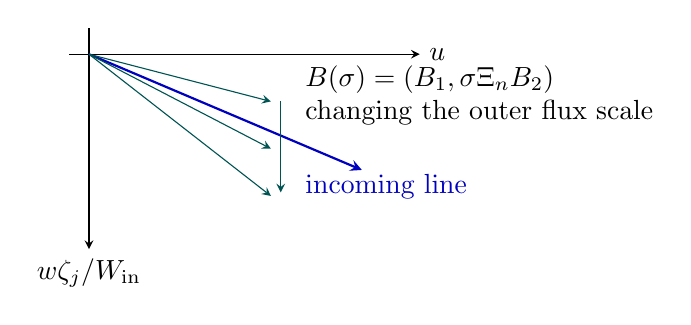
\begin{tikzpicture}[x=2.1cm,y=1.5cm,>=stealth]
\draw[->] (-.12,0)--(2,0) node[right] {$u$};
\draw[->] (0,.22)--(0,-1.65) node[below] {$w\zeta_j/W_{\rm in}$};
\draw[thick,blue!75!black,->] (0,0)--(1.65,-.98);
\node[anchor=west,blue!75!black] at (1.25,-1.12) {incoming line};
\draw[teal!65!black,->] (0,0)--(1.1,-.4);
\draw[teal!65!black,->] (0,0)--(1.1,-.8);
\draw[teal!65!black,->] (0,0)--(1.1,-1.2);
\draw[->,teal!65!black] (1.16,-.4)--(1.16,-1.17);
\node[anchor=west,align=left] at (1.25,-.35)
 {$B(\sigma)=(B_1,\sigma\Xi_nB_2)$\\changing the outer flux scale};
\end{tikzpicture}
\caption{Height selection in the two-dimensional boundary-state plane.
The incoming slope stays in a fixed negative interval.  A small angle
can therefore occur only for a short interval of the height parameter,
even when the height contrast $\Xi_n$ is very large or very small.}
\label{fig:height-selection}
\end{figure}

Normalize the natural endpoint line in its local $(u,\zeta_j)$ frame
to $(B_1,B_2)$.  In the common frame it is
$B(\sigma)=(B_1,\sigma\Xi_nB_2)$; this is the geometric content of
Figure~\ref{fig:height-selection}.  If $B_1=0$, its angle with
$(1,a)$ is bounded below.  Otherwise write
$b_\sigma=\sigma\Xi_nB_2/B_1$.  The ideal angle sine is
\[
 \frac{|a-b_\sigma|}{\sqrt{1+a^2}\sqrt{1+b_\sigma^2}}.
\]
A small value forces $b_\sigma$ into a fixed negative compact interval,
where $|b_\sigma'|=|b_\sigma|/\sigma$ is bounded below.  Thus the set
where this angle is less than $2\delta_n$, with
$\delta_n=c_0e^{-n^2}$, lies in an interval of length at most
$C\delta_n$.  The true incoming state is $(1,a)+O(\eta_{n,j})$;
normalization is Lipschitz near these vectors.  Equation
\eqref{eq:rad-eq-js14} therefore gives the same excluded-interval bound
for a true matching angle below $\delta_n$.
All constants are independent of the other height ratios.

\begin{lemma}[Simultaneous height selection]\label{lem:radial-product-selection}
At each endpoint one can choose all $\sigma_n\in[1,2]$ so that for
every even $j\in\mathcal I_n$ the incoming and natural endpoint
lines have angle sine at least $\delta_n=c_0e^{-n^2}$ in the common
state of \eqref{eq:rad-eq-js7}.
\end{lemma}
\begin{proof}
The union of the excluded sets has measure less than one, because
\begin{equation}\label{eq:rad-eq-js13}
 \sum_{n\ge N}C\#\mathcal I_n\delta_n
 \le CC_*c_0\sum_{n\ge N}q_ne^{-n^2/2}<\tfrac12
\end{equation}
for sufficiently large $N$.
More explicitly, for a finite set of bands fix all later ratios to one
and use Lebesgue measure on the finite cube of remaining ratios.
Fubini's theorem applies the uniform one-coordinate exclusion estimate
to each condition, and the union bound gives a good choice.
Extend those finite choices by ones and take a coordinatewise convergent
subsequence.  At any fixed frequency the finite-prefix transfer is
continuous, and the deep continued fraction proved above contracts
uniformly over all height choices.  Hence the natural line is continuous
in the product topology.  Each good-angle condition is closed and
survives the limit.  The two endpoints can be chosen independently.
\end{proof}

We have now constructed smooth flat tails with a quantitative endpoint
line at every frequency.  We have not yet claimed that gluing them to
the central oscillator preserves all the spectral gaps.  That global
question is addressed next.  Its answer uses both parts of the present
construction: the selected angle at the transition cell, and the strong
attenuation through the preceding positive cap.

\section{An inverse on one fixed annulus}
\label{sec:radial-reference-inverse}

Local spectral gaps do not automatically survive gluing.  A homogeneous
solution can leave one piece, return through its neighbor, and satisfy a
new matching condition.  We must therefore estimate the global matching
problem, not just list the inverses of its pieces.

The frequency decomposition from the preceding section makes this
possible.  At a fixed frequency there are three regions: an inner
collection of well-separated models, one transition cell at each end,
and two deep tails.  The selected height ratios control the matching
angle at the transition cells.  A positive interval just before each
transition prevents its possibly large response from reaching the fixed
interior.  Figure~\ref{fig:frequency-regions} shows this division of labor.
The position of the division changes with frequency; the surface itself
will be chosen once.

\begin{figure}[htbp]
\centering
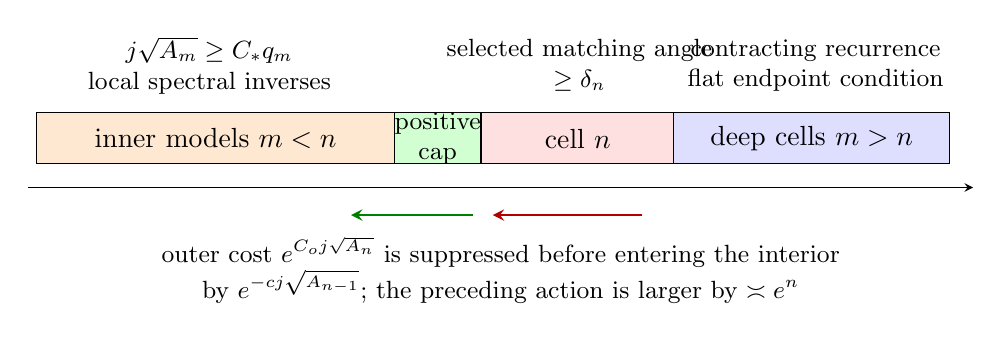
\begin{tikzpicture}[x=1cm,y=1cm,>=stealth]
\draw[->] (0,0)--(12,0);
\draw[fill=orange!18] (.1,.3) rectangle (4.65,.95);
\draw[fill=green!18] (4.65,.3) rectangle (5.75,.95);
\draw[fill=red!12] (5.75,.3) rectangle (8.2,.95);
\draw[fill=blue!13] (8.2,.3) rectangle (11.7,.95);
\node at (2.38,.62) {inner models $m<n$};
\node[align=center,font=\small] at (5.2,.62) {positive\\cap};
\node at (6.98,.62) {cell $n$};
\node at (9.95,.62) {deep cells $m>n$};
\node[align=center,font=\small] at (2.3,1.55)
 {$j\sqrt{A_m}\ge C_*q_m$\\local spectral inverses};
\node[align=center,font=\small] at (7,1.55)
 {selected matching angle\\$\ge\delta_n$};
\node[align=center,font=\small] at (10,1.55)
 {contracting recurrence\\flat endpoint condition};
\draw[->,thick,red!70!black] (7.8,-.35)--(5.9,-.35);
\draw[->,thick,green!50!black] (5.65,-.35)--(4.1,-.35);
\node[align=center,font=\small] at (6,-1.05)
 {outer cost $e^{C_o j\sqrt{A_n}}$ is suppressed before entering the interior\\
 by $e^{-c j\sqrt{A_{n-1}}}$; the preceding action is larger by $\asymp e^n$};
\end{tikzpicture}
\caption{The frequency-dependent decomposition of one end.
The other end is treated simultaneously.  Costs whose output remains
in cell $n$ or farther out can be absorbed by the coefficient weight
there; costs returning to the interior require the preceding positive cap.}
\label{fig:frequency-regions}
\end{figure}

\subsection{Joining the distinguished solution first}
\label{subsec:rad-cone-bump-target-match}

We first finish the actual geometry, keeping its second mode exactly.
On a positive interval put $y=\log r$, $w=re^f$, and prescribe the
logarithmic slope $k=\phi_y/\phi$ of a nonvanishing second-mode solution.
The equation $L_2\phi=0$ is equivalent to
\begin{equation}\label{eq:rad-eq-sp1}
 f_y=\frac{k^2+k_y-4}{4-k},\qquad
 1+f_y=\frac{k^2-k+k_y}{4-k}.
\end{equation}
Thus choosing $k<4$ and $k^2-k+k_y>0$ constructs both the solution and
a positive-curvature connector: integrate $f_y$ and then
$\phi_y=k\phi$.  This is more reliable than interpolating $w$ and
hoping to retain its kernel.

The central slopes tend with all fixed derivatives to $2$ on the left
and $-2$ on the right, by \eqref{eq:rad-eq-sc2}.  Cut sufficiently far
out and interpolate $k$ to the respective constant on a unit $y$
interval.  At either constant the second expression in
\eqref{eq:rad-eq-sp1} equals one, so $C^1$ closeness ensures
$1+f_y\ge3/4$.  Smooth cutoffs match all endpoint germs.
The connector ends in an exact cone, where $k=\pm2$.

On the auxiliary cone of a selected tail, the natural second-mode
solution is $C_+r^2+C_-r^{-2}$.  At the right tail the incoming line
is $r^2$, so the selected nonzero angle implies $C_-\ne0$.
Far toward $r=0$ the natural slope therefore tends to $-2$.
At the left tail the incoming line is $r^{-2}$, and the slope tends
to $2$ toward $r=\infty$.  In both cases the solution is nonzero
sufficiently far along the cone.  The same interpolation of $k$
connects it to an exact cone while retaining $1+f_y\ge3/4$.
Arbitrarily long exact cone segments may be placed between these short
connectors.

A radius change
\begin{equation}\label{eq:rad-eq-ha1}
 \widetilde r=Rr,\qquad \widetilde w(Rr)=Rw(r)
\end{equation}
places each tail at the required radius and preserves $w/r$, $B_j$ and
$\varpi\,dr$.  A subsequent positive height rescaling matches the
additive constant in $f$ without changing homogeneous solutions or
travel angles.  Scaling the tail solution matches its nonzero value.
We obtain one smooth profile $w_*$ and one globally defined, endpoint-flat
second-mode solution $\phi_*$.  We write $w=w_*$ for the rest of this
section.  Only positive pieces have been added, so all
negative travel angles remain those already computed.
What remains to prove is that there is no additional kernel and that
the inverse estimates are uniform.

\subsection{What a positive buffer does to a model inverse}

A useful local fact is that a distant boundary condition produces an
exponentially small change at a cut inside a positive region.  We need
this fact for the operator and for its boundary derivatives, including
the bordered central model.

\begin{lemma}[Cutting inside a positive buffer]\label{lem:fence-compression}
Let $H_0=-\partial_X^2+V$ have a self-adjoint full-model realization.
Allow also a compact symmetric scalar border, supported away from all
cuts.  Suppose the resulting operator $\mathcal H$ is invertible with
$\|\mathcal H^{-1}\|\le B_0$.  At each of at most two cuts $i$, suppose
$V\ge m_i^2$ on the exterior and on an inward interval of length
$(S_i+6)/m_i$.  Suppose $V\le Cm_i^2$ on the cut layer and the inner
cutoff layer, each of width $4/m_i$; any finite exterior wall is at
least $4/m_i$ away.

Let $\alpha_i^{\rm in}$ be the unit-boundary energy of the inward
positive interval with an artificial Dirichlet wall, and
$\alpha_i^{\rm out}$ that of the exterior with its natural condition.
Then $\alpha_i^{\rm in},\alpha_i^{\rm out}\asymp m_i$.
With $D=\operatorname{diag}(\alpha_i^{\rm in}+\alpha_i^{\rm out})$,
the retained Dirichlet operator $\mathcal H_D$, its row-zero Poisson
map $T$, and its outward derivative matrix $\Lambda$ satisfy
\begin{equation}\label{eq:buffer-estimates-new}
 \begin{gathered}
 \|\mathcal H_D^{-1}\|\le B_0+C\sum_i m_i^{-2},\qquad
 \|TD^{-1/2}\|\le C\Bigl(\sum_i m_i^{-2}\Bigr)^{1/2},\\
 D^{-1/2}\bigl(\Lambda-\operatorname{diag}\alpha_i^{\rm in}\bigr)D^{-1/2}
       =O(E),\qquad
 |E_{ik}|\le CB_0m_im_ke^{-S_i-S_k},
 \end{gathered}
\end{equation}
provided $B_0m_i^2e^{-S_i}$ is sufficiently small at every cut.
In particular $\Lambda$ is positive.
\end{lemma}

\begin{proof}
The unit-boundary energy is at least $m_i$ by expanding
$\int|v'\pm m_iv|^2$.  A test function supported within distance
$2/m_i$ gives the matching upper bound.  Join the inward and exterior
unit solutions at the cut; after division by
$\alpha_i^{\rm in}+\alpha_i^{\rm out}$ this is its local point-source
Green function.  Cut it off just before the inner artificial wall,
obtaining $K_i$.  Positive comparison with $-v''+m_i^2v=0$ gives
\[
 \mathcal H(K_i,0)=(\delta_{c_i}+f_i,0),\qquad
 \|K_i\|_2\le Cm_i^{-3/2},\qquad
 \|f_i\|_2\le Cm_i^{1/2}e^{-S_i}.
\]
The scalar coordinate is omitted in the unbordered case; in the bordered
case the cutoff support is disjoint from the border.  The residual is
an ordinary $L^2$ commutator source, not a point source.  Therefore
\[
 \boldsymbol g_i=(K_i,0)-\mathcal H^{-1}(f_i,0)
\]
is the exact Green column at the cut.

Let $\Gamma_{ik}=(g_k)_{\rm field}(c_i)$.  The correction is homogeneous
in the positive buffer at cut $i$ and satisfies the natural exterior
condition.  Propagating it from the inner cutoff layer to the cut costs
a further $e^{-S_i}$; rescaling a layer of width $m_i^{-1}$ converts
its $L^2$ bound to a point bound with factor $Cm_i^{1/2}$.
Consequently
\[
 D^{1/2}\Gamma D^{1/2}=I+E,\qquad
 |E_{ik}|\le CB_0m_im_ke^{-S_i-S_k}.
\]
This also follows directly by applying Green's identity to the two
commutator residuals.  The stated smallness makes this finite matrix
invertible.

Let $\iota$ extend the retained source by zero and $\mathcal R$ restrict
the field, preserving the scalar in both cases.  Subtracting the cut
values gives the exact formulas
\[
 \mathcal H_D^{-1}=\mathcal R\mathcal H^{-1}\iota
                     -\boldsymbol g_I\Gamma^{-1}\boldsymbol g_I^*,
 \qquad T=\boldsymbol g_I\Gamma^{-1}.
\]
There is no hidden kernel: extending a homogeneous Dirichlet field by
zero leaves only cut delta sources, and the invertible cut matrix forces
their coefficients to vanish.  Moreover
\[
 \|\boldsymbol g_iD_{ii}^{1/2}\|
 \le C(m_i^{-1}+B_0m_ie^{-S_i})\le Cm_i^{-1},
\]
which proves the first two bounds.  Interior and exterior derivatives
of a Green column add to its delta coefficient, so
$\Lambda=\Gamma^{-1}-\operatorname{diag}\alpha_i^{\rm out}$.
This gives the final estimate and positivity.  The compact symmetric
border cancels in the same Green identities, so the proof covers it
without an additional boundary term.
\end{proof}

We now translate this estimate to the radial problem.  The exact norm
and flux conversions are
\begin{equation}\label{eq:rad-eq-hn2}
 \|u\|_{L^2(\varpi dr)}^2=12\lambda\int\upsilon^2|\psi|^2\,dX,
 \qquad wu_r=\lambda\sqrt{\mathcal P}
       \left(\psi_X-\frac{\mathcal P_X}{2\mathcal P}\psi\right).
\end{equation}
Using $\sqrt\lambda\psi$ removes the absolute profile amplitude.
For a Morse cell the short and long positive cut regions have,
respectively,
\[
 (m_{X,j},\Delta X,\upsilon)
 \asymp(j\sqrt{A_m},1,A_m),\qquad
 (jA_m^{9/2},A_m^{-4},A_m^5).
\]
Each contains action $c\tau_{m,j}$ with
$\tau_{m,j}=j\sqrt{A_m}$, and $\upsilon/m_{X,j}\le C/j$.
The full-model inverse costs a fixed power of $\mathcal E_m$.
For the central oscillator, far cuts have
$m_{X,j}\asymp j|X|$ and action $cjX^2$; its two-sided weighted
inverse was proved in the preceding section.

The Liouville factor also changes the leading conormal impedance.
At a central cut with outward sign $\epsilon_i$, the exact radial
boundary matrix is
\begin{equation}\label{eq:rad-eq-hn3}
 \Lambda_r=\lambda\operatorname{diag}(\sqrt{\mathcal P_i})
                  \Lambda_X\operatorname{diag}(\sqrt{\mathcal P_i})
          +\lambda a_c\operatorname{diag}(\epsilon_i\mathcal P_i).
\end{equation}
Thus its positive diagonal is
$\kappa_i=\lambda\mathcal P_i(\alpha_i^{\rm in}+\epsilon_i a_c)$,
comparable to $\lambda\mathcal P_i m_{X,j}$ at the chosen far cuts.
For a Morse model it is simply $\lambda\alpha_i^{\rm in}$.
Retaining this gauge term is necessary for exact flux matching.

\subsection{The inner region: retain the full positive interface energy}
\label{subsec:rad-localized-hilbert-assembly}

Fix $j\in\mathcal I_n$.  The finite inner domain consists of the
central model, the earlier cells $m<n$, and their positive connectors.
Its two outer boundaries are the entrances to the selected transition
joins.  Impose zero values there.  At frequency two use the auxiliary
compact symmetric border.  In radial Hilbert notation,
\begin{equation}\label{eq:rad-eq-hn1}
 d\mu=\varpi\,dr,\qquad B_j=-\varpi^{-1}L_j,
 \qquad F=-\varpi^{-1}f,\qquad
 \langle u,F\rangle_{L^2(d\mu)}=-\int\overline u f\,dr.
\end{equation}
For a border column $k=-\varpi^{-1}g_0$, its Hilbert adjoint is
$k^*u=-\ell_0u$; changing the sign of the scalar source row therefore
makes the border symmetric.  This convention will be used in all
intermediate energy identities.

Let $D_h$ be the direct sum of the cut-model Dirichlet inverses and
the exact positive-connector inverses.  On every positive connector,
\begin{equation}\label{eq:rad-eq-hn5}
 Q_j(u)=\int\left(w|u_r|^2+j^2\frac{w'}r|u|^2\right)dr
               \ge cj^2\|u\|_{L^2(d\mu)}^2.
\end{equation}
Here $c=1/6$ on the short joins where $rw'/w\ge2$, and a smaller
fixed positive $c$ covers the cone heads and central connectors.
Its Poisson map $P_C$ and full conormal matrix $\Lambda_C$ consequently
satisfy $\|P_Ca\|\le(C/j)(a^*\Lambda_Ca)^{1/2}$.

A short connector can have a large mixed entry in $\Lambda_C$.
We keep that entry instead of treating it as an error.  At all internal
interfaces set
\begin{equation}\label{eq:rad-eq-hn6}
 S_0=\operatorname{diag}(\kappa_i)+\bigoplus_C\Lambda_C,
 \qquad S=S_0+E_h.
\end{equation}
The positive matrix $S_0$ has blocks of size at most two and dominates
$D_\kappa=\operatorname{diag}(\kappa_i)$.  All errors $E_h$ now
come from crossing positive buffers inside the local models.

To see this uniformly in the number of cells, use a source weight $W$
which is one on the finite middle and has cell size
\begin{equation}\label{eq:rad-eq-hn4}
 W_m=(\mathcal E_m/\mathcal E_N)^{M_0}(H_m/H_N)^{-\gamma}.
\end{equation}
Make it constant across each whole positive gap, with the geometric
mean of the neighboring weights, and vary it inside the model cells.
For $|\gamma|\le1$,
\begin{equation}\label{eq:adjacent-weight-ratio-new}
 |\log(W_{m+1}/W_m)|
 \le Cm^2+CM_0m^{3/2}\log(e+m).
\end{equation}
Thus this interpolation changes cell norms by fixed coefficient powers.
Let $\Omega=\operatorname{diag}(W(c_i))$.  It commutes with $S_0$,
because the two ends of every positive connector have the same weight.

The buffer lemma and \eqref{eq:rad-eq-hn2} give local normalized errors
\begin{equation}\label{eq:rad-eq-hn7}
 \mathcal E_m^{C(M_0)}\langle j\rangle^C e^{-c\tau_{m,j}},\qquad
 C\langle j,X_0\rangle^Ce^{-cjX_0^2},\qquad
 C_N\langle j\rangle^Ce^{-cjL}
\end{equation}
for earlier cells, central cuts and initial cone heads.  The leading
Poisson layer at a model cut has Hilbert norm at most
$(C/j)\sqrt{\kappa_i}|a_i|$, because
$\upsilon/m_{X,j}\le C/j$.  Its remaining part has the first type
of error in \eqref{eq:rad-eq-hn7}.  The assertion of uniform smallness
includes frequencies arbitrarily far above a cell's threshold.  To see
this, put $t=j\sqrt{A_m}\ge C_*q_m$.  Since
$\log\langle j\rangle\le\log(1+t)+Cm^2$, the logarithm of that
local error is bounded, with fixed $a,b,c>0$, by
\begin{equation}\label{eq:inner-uniform-suppression}
 a q_m+b\log(1+t)-ct
 \le a q_m-\tfrac34ct+C_b
 \le-\tfrac12ct+C_b
 \quad\text{if }C_*\ge4a/c.
\end{equation}
Here $m^2=o(q_m)$ was included in $a$, and the middle inequality uses
$b\log(1+t)\le ct/4+C_b$.  Increasing $N$ now makes the original error
smaller than any prescribed positive tolerance, simultaneously for all $m<n$
and all such $j$.  Thus we choose $M_0$ for source conversion, then
$C_*$, then $N$, and finally the central cuts and the fixed head
lengths.  Their errors in \eqref{eq:rad-eq-hn7} have the same
polynomial-versus-exponential comparison, on the finitely many central
pieces.

Let $T_h$ be the homogeneous interpolation of common interface values,
with zero scalar row.  The resulting two estimates are
\begin{equation}\label{eq:rad-eq-hn8}
 \begin{gathered}
 \|S_0^{-1/2}\Omega^\epsilon E_h\Omega^{-\epsilon}S_0^{-1/2}\|<1/2,\\
 \|W^\epsilon T_h\Omega^{-\epsilon}S_0^{-1/2}\|\le C/j,
 \qquad \epsilon=\pm1.
 \end{gathered}
\end{equation}
For the first, normalize each model error by its two adjacent
$\kappa_i^{1/2}$.  Each interface belongs to at most two such blocks,
so their sum has operator norm at most twice the largest local norm.
Then use $\|S_0^{-1/2}D_\kappa^{1/2}\|\le1$ on both sides.
For the second, sum the squared local Poisson norms over disjoint model
interiors and over the positive connectors, whose overlap is bounded.
This proves both estimates independently of the number of cells.

The outgoing interface flux of a zero-boundary source solution is
$-T_h^*F$.  Matching values and fluxes therefore gives the exact inverse
\begin{equation}\label{eq:rad-eq-hn9}
 G_h=D_h+T_hS^{-1}T_h^*.
\end{equation}
The two signs of the weight in \eqref{eq:rad-eq-hn8} control the second
term by duality.  Local Dirichlet costs are coefficient powers, so,
for a sufficiently large fixed $M_1$,
\begin{equation}\label{eq:inner-inverse-estimates-new}
 \|W_1G_hW^{-1}\|\le C,\qquad
 \|W^{\pm1}G_hW^{\mp1}\|\le\mathcal E_n^C,
 \qquad W_1=W(\mathcal E/\mathcal E_N)^{-M_1}.
\end{equation}
The first estimate is localized and will handle ordinary inner sources.
Its net output coefficient exponent is $M_0-M_1$; at the end we rename
$M_1-M_0>0$ as the output exponent in
Proposition~\ref{prop:rad-fixed-theorem}.
The coarser second estimate is used only on boundary residuals which
already contain an exponentially small factor.  Invertibility of the
Dirichlet blocks and of $S$ proves both inverse identities in
\eqref{eq:rad-eq-hn9}; its symmetry is the corresponding Green identity.

\subsection{The transition region and an outer inverse without division by height}

The outer core begins at a selected join, contains cell $n$, and ends
where the deep tail starts.  The preceding large positive cap belongs
to the inner domain.  On the right the deep entrance is a mass entrance;
on the left it is the initial resistance entrance described earlier.
Let $r_o$ increase outward, use positive measure $dr_o$, and choose
$\lambda>0$ with $e^{-Cn^2}\le\lambda/\lambda_n\le e^{Cn^2}$.
In the state $(u,z)$, $z=wu_{r_o}/\lambda$, the core has the bounds
\begin{equation}\label{eq:transition-inputs-new}
 \begin{gathered}
 \|T\|+\|T^{-1}\|\le\mathcal K_n:=e^{Cn^2+C_o\tau_{n,j}},
 \qquad \int_{\rm core}\varpi\,dr_o\le\lambda e^{Cn^2},\\
 \|P_d\|_{L^2(d\mu)}\le\sqrt\lambda e^{Cn^2},
 \qquad \|B_{d,D}^{-1}\|\le Cj^{-4}.
 \end{gathered}
\end{equation}
Here $P_d$ is the deep natural solution with entrance value one.

For clarity, these four estimates follow from different parts of the
construction.  The last is \eqref{eq:rad-eq-rm20}.
The core mass is $12\lambda_n\int(v/r)^2dX$, plus the negligible
joining masses, so it has the stated size by
\eqref{eq:rad-eq-rm6}.  The weighted node contraction
\eqref{eq:rad-eq-dg4} bounds the squared norm of $P_d$ by the first
deep mass.  If an initial resistance edge comes first, its next mass
height is at most $C/(\Lambda\mu R_0)$ and the edge mass is small;
the same bound follows.
For the transfer estimate, on a positive piece the off-diagonal
coefficients in $(u,z)$ are $\lambda/w$ and $j^2w_r/(\lambda r)$.
Balancing their integrals bounds the transfer in either direction by
\[
 e^{Cn^2}\exp\!\left(2j\sqrt{\left(\int dr_o/w\right)
                                  \left(\int w_r\,dr_o/r\right)}\right).
\]
The product inside the square root is $O(A_n)$ on either positive cap
and smaller on the short join.  On the negative component use
$u_{XX}+j^2\rho u=0$ and the energy
$E=|u_X|^2+(1+j^2\rho)|u|^2$.
It satisfies
$|E_X|\le[1+j^2|\rho_X|/(1+j^2\rho)]E$.
The interval has length $O(n^2)$ and $\rho$ has one peak, so the
integrated second term is at most $2\log(1+j^2\max\rho)$.
Converting the flux back to $(u,z)$ costs only $e^{Cn^2}$.
Together these estimates prove \eqref{eq:transition-inputs-new}.

The natural outer solution may vanish at the entrance.  A logarithmic
slope there is therefore the wrong variable.  Normalize its full state:
\begin{equation}\label{eq:rad-eq-tm1}
 v=(V(r_{o,-}),f_V(r_{o,-})/\lambda),\qquad |v|=1,
 \qquad f_u=wu_{r_o},\qquad v^\perp=(-v_2,v_1).
\end{equation}
Let $U$ have entrance state $v^\perp$.  For $\mathscr H_j=-L_j$,
the kernel
\[
 K_o(r_o,t_o)=\lambda^{-1}U(\min(r_o,t_o))V(\max(r_o,t_o))
\]
has the natural endpoint condition and the complementary Robin condition
$v\cdot(u,f_u/\lambda)=0$ at the entrance.  Its normalization is exact:
$w(UV_{r_o}-U_{r_o}V)=-\lambda$.
Thus
\begin{equation}\label{eq:outer-robin-new}
 R_oF=\int K_o(r_o,t_o)F(t_o)\,d\mu(t_o),\qquad
 G_of=-\int K_o(r_o,t_o)f(t_o)\,dt_o
\end{equation}
are respectively the Hilbert inverse of $B_j$ and the original-source
inverse of $L_j$.  No entrance height has been divided out.
Green's identity gives the remaining boundary equation
\begin{equation}\label{eq:rad-eq-tm2}
 v^\perp\cdot(u,f_u/\lambda)
       =\lambda^{-1}\int V\varpi F\,dr_o,
 \qquad \|V\|_{L^2(d\mu)}\le\sqrt\lambda\mathcal E_n^C\mathcal K_n.
\end{equation}
The natural endpoint term is zero by the deep-tail construction.

The factor $\lambda^{-1}$ in the kernel causes no amplitude loss.
On the core it is canceled by the mass bound in
\eqref{eq:transition-inputs-new}.  On the deep region exact kernel
restriction gives
\[
 (R_o)_{d,d}=B_{d,D}^{-1}+P_dK_o(r_{o,+},r_{o,+})P_d^*,
 \qquad |K_o(r_{o,+},r_{o,+})|
        \le\lambda^{-1}\mathcal E_n^C\mathcal K_n^2.
\]
The two Poisson norms cancel it there, and the cross blocks have one
Poisson factor each.  Consequently
\begin{equation}\label{eq:rad-eq-tm3}
 \|R_o\|\le\mathcal E_n^C\mathcal K_n^2.
\end{equation}
The localized deep kernel \eqref{eq:rad-eq-dj5} and the outward
homogeneous quotient \eqref{eq:rad-eq-rm17} give more precisely
\begin{equation}\label{eq:rad-eq-tm4}
 \|\vartheta_kR_o\vartheta_m\|
 \le\mathcal E_k^C\mathcal E_m^C\mathcal K_n^2 e^{-|S_k-S_m|},
 \qquad k,m\ge n-O(1).
\end{equation}
A product of two outward quotient factors is bounded by the same
exponential, since both indices lie beyond the entrance.
Converting the source and target to $L^2(dr_o)$ adds
$\varpi^{-1/2}$ on each of their cells, bounded by coefficient powers.
Hence \eqref{eq:rad-eq-tm4} also holds for $G_o$ in ordinary source
units.  These observations justify both inverse identities and
reciprocity directly from the kernel.

\subsection{The two boundary values which remain to be matched}
\label{subsec:terminal-matching}

At each truncation boundary use the scale
$\lambda_i=j^2W_{{\rm in},i}/r_{{\rm in},i}$.
Its ratio to the transition-cell height is between $e^{-Cn^2}$ and
$e^{Cn^2}$, so the preceding outer estimates apply.
Let $\kappa_i$ be the impedance of the artificial incoming positive
block used for height selection and put
$d_i=\kappa_i/\lambda_i$, $D_0=\operatorname{diag}(d_i)$.
The incoming estimate gives $0<d_i\le1/2$; in the first band $d_i=1/j$.
Use normalized boundary coordinates
$x_i=\sqrt{\lambda_i}u_i$, $z_i=f_{u,i}/\sqrt{\lambda_i}$.

Let $\mathcal B_h$ denote the inner Hilbert operator, including its
symmetric scalar border, and let $\mathcal Q_h$ be its quadratic form.
We need to know how much the true inner derivative matrix differs
from this artificial incoming one.  Take its positive-block Poisson
function of boundary height $\lambda_i^{-1/2}$, cut it off near the
inner end of that block, and extend by zero.  Call the resulting field
$\mathcal L_i$, and its ordinary Hilbert residual
$\mathcal F_i=\mathcal B_h\mathcal L_i$, including zero scalar row.
Allocate separate fixed fractions of the preceding cap to this cutoff
and to the earlier model's buffer.  Positive comparison and the
commutator
\[
 \mathscr H_j(\chi u)-\chi\mathscr H_ju
       =-2w\chi'u'-(w\chi')'u
\]
then give
\begin{equation}\label{eq:rad-eq-tm6}
 \begin{gathered}
 \|W^{\pm1}\mathcal L_i\omega_i^{\mp1}\|
       \le C\sqrt{d_i}/j,\qquad
 \|W^{\pm1}\mathcal F_i\omega_i^{\mp1}\|
       \le\sqrt{d_i}\mathcal E_n^Ce^{-S_{b,i}},\\
 S_{b,i}=c\tau_{n-1,j}\quad\text{or, in the first band, }cjL.
 \end{gathered}
\end{equation}
Here $\omega_i$ is the constant weight on this positive gap.
The first bound uses the energy $\kappa_i/\lambda_i=d_i$ and
\eqref{eq:rad-eq-hn5}; the second uses the extra attenuation on the
cutoff layer.  The two lifts have disjoint supports, and their energy
matrix is diagonal with entries
$d_i(1+O(\mathcal E_n^Ce^{-2S_{b,i}}))$.

The exact homogeneous Poisson map is
$P_h=\mathcal L-G_h\mathcal F$.
Completing the quadratic form gives the true normalized derivative
matrix
\begin{equation}\label{eq:rad-eq-tm7}
 D_b=\mathcal Q_h(\mathcal L,\mathcal L)-\mathcal F^*G_h\mathcal F
       =D_0+E_b,
 \qquad |(E_b)_{ik}|\le
     \mathcal E_n^C\sqrt{d_id_k}e^{-S_{b,i}-S_{b,k}}.
\end{equation}
The two cross terms cancel one correction term because
$\mathcal B_hG_h\mathcal F=\mathcal F$ and the correction has zero
boundary values.  This identity is also why the error has \emph{two}
attenuation factors.  The scalar border is symmetric and every lift
has row zero, so there is no missing scalar term.

Use the outer normalized states \eqref{eq:rad-eq-tm1} with these
$\lambda_i$.  Let $A=\operatorname{diag}(v_{1,i})$,
$B=\operatorname{diag}(v_{2,i})$, and let $\mathcal V$ consist of
the two outer columns $V_i/\sqrt{\lambda_i}$.
The inner source flux is $-P_h^*F_h$, while
\eqref{eq:rad-eq-tm2} supplies the outer equation.  Thus the complete
matching problem is just
\begin{equation}\label{eq:rad-eq-tm8}
 z=D_bx-P_h^*F_h,\qquad -Bx+Az=\mathcal V^*F_o,\qquad
 Kx=\mathcal V^*F_o+AP_h^*F_h,\quad K=A(D_0+E_b)-B.
\end{equation}

The angle selected in the preceding section is exactly what is needed
to invert the diagonal part of $K$.  Its state is
$(u,-u\pm f_u/\lambda_i)$; the change to $(u,f_u/\lambda_i)$
has a fixed condition number.  Transport across the nearly identity
join preserves the angle lower bound up to a fixed factor.  Hence
\begin{equation}\label{eq:rad-eq-tm9}
 |v_{1,i}d_i-v_{2,i}|
 =\sqrt{1+d_i^2}\,|\sin\angle(v_i,(1,d_i))|
 \ge c\delta_n.
\end{equation}
This argument remains valid when $v_{1,i}=0$.
Any later dependence of the central connectors on the selected tails
is confined to $E_b$; the artificial incoming direction itself was
fixed before the height parameter was varied.

Two estimates now decide the choice of scales:
\begin{equation}\label{eq:rad-eq-tm10}
 \delta_n^{-1}\|E_b\|<c/4,\qquad
 \mathcal E_n^C\delta_n^{-1}
     e^{C_o\tau_{n,j}-c\tau_{n-1,j}}<1/4.
\end{equation}
The first makes $K$ invertible.  The second controls responses which
return to the fixed interior.  They are compatible because
\[
 \tau_{n-1,j}/\tau_{n,j}\asymp e^n,\qquad
 \tau_{n-1,j}\ge C_*q_{n-1},\qquad
 q_n/q_{n-1}\to1,\qquad n^2/q_{n-1}\to0.
\]
Choose $C_*$ after the fixed coefficient exponent, then $N$ large.
The first relation absorbs $C_o\tau_{n,j}$ into a quarter of the
preceding action, and the other relations absorb $Cq_n+n^2+|\log c_0|$
into another quarter.  The first estimate has two such attenuations
by \eqref{eq:rad-eq-tm7}.  At the finite initial band choose the fixed
cone-head length $L$ large enough instead.  Therefore
$\|K^{-1}\|\le C\delta_n^{-1}$ uniformly in the band and frequency.

\subsection{The global estimate and the order of choices}

Set $K_1=A+BD_b$.  Solving \eqref{eq:rad-eq-tm8} and reconstructing
the outer homogeneous coefficient gives the exact matched inverse
\begin{equation}\label{eq:rad-eq-tm11}
 G=\begin{pmatrix}G_h&0\\0&R_o\end{pmatrix}
  +\begin{pmatrix}P_h&0\\0&\mathcal V\end{pmatrix}
   \begin{pmatrix}
       K^{-1}A&K^{-1}\\K^{-T}&K_1K^{-1}
   \end{pmatrix}
   \begin{pmatrix}P_h^*&0\\0&\mathcal V^*\end{pmatrix}.
\end{equation}
For example, the outer coefficient is
$K_1x-BP_h^*F_h$.  Since $D_b=D_b^T$, $A,B$ commute and
$A^2+B^2=I$, direct multiplication gives
\[
 KA=AK^T,\qquad K^TK_1=K_1^TK,\qquad
 K_1K^{-1}A-B=K^{-T}.
\]
These identities prove both the formula and the symmetry of its middle
matrix, whose norm is $O(\delta_n^{-1})$.
We choose equal boundary weights at the two ends by using their common
band index.  A bounded index shift changes their ratio only by a
coefficient power and has the same estimates.

There are two ways to pay for a boundary correction.  We give the
weighted estimate explicitly for each, because this is where local
inverse bounds become an estimate on the whole annulus.

\paragraph{An outer block and its coefficient weights.}
First consider terms involving only $R_o$, $\mathcal V$ and the leading
lifts $\mathcal L$.  Their source and output indices are at least
$n-O(1)$.  Combining \eqref{eq:rad-eq-tm4} with
$\|K^{-1}\|\le C\delta_n^{-1}$ gives, after increasing fixed constants,
\[
 \|\vartheta_kG_{\rm out}\vartheta_m\|
 \le C\exp\{a(q_k+q_m)+d q_n-|S_k-S_m|\}.
\]
Here $d$ includes the finite-core cost: indeed
$\delta_n^{-1}e^{C_o\tau_{n,j}}
 \le c_0^{-1}\exp(n^2+C_oC_*q_n)$.
Since the output is outer, $q_n\le c_1q_k+C_1$; write $d_1=dc_1$.
For $\Delta S=S_k-S_m$, conjugation by the source and output weights
therefore gives the following exact exponent bound:
\begin{equation}\label{eq:outer-weighted-block}
 \begin{aligned}
 \log\|\vartheta_kW_1G_{\rm out}W^{-1}\vartheta_m\|
 &\le C-(M_1-2a-d_1)q_k\\
 &\quad +(a-M_0)(q_m-q_k)-|\Delta S|+\gamma\Delta S.
 \end{aligned}
\end{equation}
Fixed neighboring-index and source-measure changes have been included
in $a,d_1,C$.  Choose $M_1>\max(M_0,2a+d_1)$, after $C_*$.
For any $0<\gamma\le\gamma_+<1$, use
\[
 |q_m-q_k|\le\varepsilon|S_m-S_k|+C_\varepsilon,
 \qquad
 \varepsilon=\frac{1-\gamma_+}{2(1+|a-M_0|)}.
\]
Then \eqref{eq:outer-weighted-block} is at most
$C_\gamma-\tfrac12(1-\gamma_+)|S_k-S_m|$.
This is a summable block kernel in both indices.  On either tail, with
$s_0=\inf_{m\ge N}(S_{m+1}-S_m)>0$ and
$\eta=\tfrac12(1-\gamma_+)$, we have
\[
 \sup_k\sum_m e^{-\eta|S_k-S_m|}
 \le1+\frac{2}{e^{\eta s_0}-1}.
\]
The same estimate holds with $k,m$ reversed.  The two endpoint copies
and the bounded overlap of the localizers change it only by a fixed
factor.  The block Schur estimate proves the outer contribution to the
desired operator bound.
Notice that increasing the output exponent works precisely because
$k$ is near or beyond the transition index; it gives no such estimate
at a fixed interior output.

\paragraph{A boundary block returning to the interior.}
The upper-right block of \eqref{eq:rad-eq-tm11} is
$P_hK^{-1}\mathcal V^*$.  Substituting
$P_h=\mathcal L-G_h\mathcal F$, its part which can reach the fixed
interior is
\[
 C_{ho}=-(G_h\mathcal F)K^{-1}\mathcal V^*.
\]
Let $\Omega$ be the common boundary weight, and use $W_h,W_o$ for
the restrictions of $W$.  The preceding estimates supply
\begin{equation}\label{eq:boundary-column-weights}
 \begin{gathered}
 \|W_hG_h\mathcal F\Omega^{-1}\|
       \le\mathcal E_n^{C_1}e^{-c\tau_{n-1,j}},\\
 \|\Omega K^{-1}\Omega^{-1}\|\le C\delta_n^{-1},\\
 \|\Omega\mathcal V^*W_o^{-1}\|
       =\|W_o^{-1}\mathcal V\Omega\|
       \le C_\gamma\mathcal E_n^{C_2}e^{C_o\tau_{n,j}}.
 \end{gathered}
\end{equation}
The first is \eqref{eq:inner-inverse-estimates-new} applied to the
residual bound \eqref{eq:rad-eq-tm6}; $d_i\le1/2$ absorbs its two
boundary factors.  The middle bound uses equal weights at the two
ends.  For the last bound, the localized column has decay
$\mathcal E_n^C\mathcal E_k^C e^{C_o\tau_{n,j}}e^{-(S_k-S_n)}$.
After either sign of the weight, its extra exponent is
$(C\pm M_0)(q_k-q_n)-(1\mp\gamma)(S_k-S_n)$.
The same slow-variation inequality used above makes its squared sum
finite, leaving a fixed coefficient power at $n$ and a constant
$C_\gamma$.  This proves the displayed adjoint estimate as well as its
reciprocal-weight version.

Multiplying the three factors in \eqref{eq:boundary-column-weights}
now exhibits the two competing costs in one operator estimate:
\begin{equation}\label{eq:one-boundary-cross-block}
 \begin{aligned}
 \|W_hC_{ho}W_o^{-1}\|
 &\le C_\gamma\mathcal E_n^C\delta_n^{-1}
             e^{C_o\tau_{n,j}-c\tau_{n-1,j}}\\
 &\le C_\gamma e^{-c\tau_{n-1,j}/2}\le C_\gamma.
 \end{aligned}
\end{equation}
The second line is the explicit exponent comparison proving
\eqref{eq:rad-eq-tm10}; enlarge the constants there before choosing
$C_*,N$.  For the initial finite band replace the preceding action by
$cjL$.  On the tails $\mathcal E/\mathcal E_N\ge1$, while its smooth extension
has a positive minimum on the fixed middle.  Thus $W_1\le C_{\rm mid}W$
with a fixed constant, which gives the required output-weight bound.
The transpose block uses the opposite sign of the weight in
\eqref{eq:boundary-column-weights}.  Terms with two residual columns
have two preceding attenuations; terms with one residual and one leading
lift have the same estimate.  Thus every correction in
\eqref{eq:rad-eq-tm11} is covered, while the direct inner term is
already bounded by \eqref{eq:inner-inverse-estimates-new}.
We conclude
\begin{equation}\label{eq:global-reference-bound-new}
 \|W_1GW^{-1}\|\le C
\end{equation}
at angular order zero, with the original source-density conversions
included by the coefficient powers already used above.

\begin{lemma}[One geometry for all flat exponents]
\label{lem:radial-uniform-exponents}
The profile, height choices, central cuts and cone-head lengths can be
chosen once so that \eqref{eq:global-reference-bound-new} holds for every
compact range $[\gamma_-,\gamma_+]\Subset(0,1)$.  Only the norm
constants and coefficient exponents may depend on that range.
\end{lemma}
\begin{proof}
Every finite matching choice uses only adjacent weight ratios.
Estimate~\eqref{eq:adjacent-weight-ratio-new} is uniform for
$|\gamma|\le1$.  Fix a source exponent $M_0$ which absorbs the
original-source conversion, then choose $C_*,N$, the central cuts
and head lengths using that uniform bound.  In particular, the
invertibility of $S$ and $K$ is independent of a compact range of
flat exponents.

After this geometry is fixed, the only new issue is the infinite
summation of the deep kernel.  Conjugation by $H^{-\gamma}$ changes
its exponential factor to
\[
 e^{-|S_k-S_m|+\gamma(S_k-S_m)}
      \le e^{-(1-|\gamma|)|S_k-S_m|}.
\]
Its row and column sums are finite when $|\gamma|\le\gamma_+<1$.
Coefficient factors are absorbed using
\[
 |q_k-q_m|\le\varepsilon|S_k-S_m|+C_\varepsilon,
\]
which follows from $q'(x)/S'(x)\to0$.
Choose $\varepsilon$ after $\gamma_+$; this changes the summation
constant and output exponent, not the geometry.  The boundary terms
which enter the interior have already acquired the attenuation in
\eqref{eq:rad-eq-tm10}.  Compact-range summation constants multiply an
existing bound and do not enter the finite matrix inversions.
Thus no later choice of endpoint exponent changes the profile.
\end{proof}

The same estimates with one radial derivative use the local equation
rather than differentiating a spectral decomposition.  On a slightly
enlarged cell,
\begin{equation}\label{eq:rad-eq-rm39}
 \begin{aligned}
 \|u_r\|_2&\le\mathcal E_m^C\bigl(\|f\|_2+(1+j)\|u\|_2\bigr),\\
 \|u_{rr}\|_2&\le\mathcal E_m^C\bigl(\|f\|_2+(1+j^2)\|u\|_2\bigr).
 \end{aligned}
\end{equation}
To derive the first, use interval interpolation
$\|u_r\|_2^2\le C\|u\|_2(\|u_{rr}\|_2+\|u\|_2)$ and substitute
$wu_{rr}=f-w'u_r+j^2w'u/r$; absorb the resulting
$C\|u\|_2\|u_r\|_2$ by Young's inequality.  Substitution back gives
the second.  Rescaling and the reciprocal profile cost coefficient
powers.  A cutoff on the enlarged interval supplies the displayed
local version without imposing a boundary condition.  At mode two
replace $f$ by $f-\nu g_0$, a compact contribution already controlled
by its scalar norm.
Thus one normal derivative uses at most one extra angular derivative.
On an outer transition region any fixed $j$ power is itself bounded
by a coefficient power, since $j<\mathcal H_n$.

\subsection{The realization, the zero mode and the final border}

We now identify the common domain and complete the statement of
Proposition~\ref{prop:rad-fixed-theorem}.

\begin{definition}[The weighted graph domain]\label{def:radial-graph-domain}
Let $\mathcal Y_\gamma^{\rm rad}$ be the source space
\eqref{eq:rad-eq-source-norm} at order zero with
$\int\langle f\rangle\,dr=0$, including its scalar row.
Let $\mathcal X_\gamma^{\rm rad}$ consist of $(u,\nu)$ with
$u=a_L\chi_L+v$ and squared norm
\[
 |a_L|^2+|\nu|^2+
 \sum_m\mathcal E_m^{-2M_1}H_m^{-2\gamma}
               \|\vartheta_mv\|_{L^2(dr\,d\theta)}^2.
\]
The angular measure is normalized.  Define
\[
 \begin{aligned}
 \mathcal D_\gamma^{\rm rad}
 &=\{(u,\nu)\in\mathcal X_\gamma^{\rm rad}:
          \mathbb L_w(u,\nu)\in\mathcal Y_\gamma^{\rm rad}\},\\
 \|U\|_{\mathcal D_\gamma^{\rm rad}}
   &=\|U\|_{\mathcal X_\gamma^{\rm rad}}
        +\|\mathbb L_wU\|_{\mathcal Y_\gamma^{\rm rad}}.
 \end{aligned}
\]
The differential expression is interpreted distributionally.  This
definition applies first to the auxiliary border and then to the final
one below.
\end{definition}

The zero mode has not entered the spectral construction.  It is solved
exactly by two primitives.  For $\int f_0\,dr=0$, set
\begin{equation}\label{eq:rad-eq-rm49}
 p_0(r)=\int_{r_-}^r f_0(t)\,dt=-\int_r^{r_+}f_0(t)\,dt,\qquad
 u_0(r)=-\int_r^{r_+}\frac{p_0(t)}{w(t)}\,dt.
\end{equation}
Then $(wu_0')'=f_0$, the right height is zero, and the left height is
an allowed constant.  Summing the cells beyond $n$ gives
$|p_0|\le\mathcal E_n^CH_n^\gamma\|f_0\|_{Y_{\gamma,0}}$.
Division by $w$ and one integration cost only coefficient powers, so
the primitive converges and has the required endpoint estimate after
subtracting $a_L\chi_L$.  The coefficient $a_L$ is a bounded source
functional.  A nonzero homogeneous flux would produce
$\int dr/w$, excluded by its growth; a constant is excluded by the
right normalization.  The zero channel is therefore unique.

\begin{lemma}[The two inverse identities and the graph closure]
\label{lem:rad-green-completion}
The matched nonzero-mode inverse \eqref{eq:rad-eq-tm11} and the zero-mode
primitive \eqref{eq:rad-eq-rm49} define
$\mathbb G_w:\mathcal Y_\gamma^{\rm rad}\to\mathcal D_\gamma^{\rm rad}$.
They satisfy
\begin{equation}\label{eq:rad-reference-piecewise-left-identity}
 \mathbb L_w\mathbb G_w=I,\qquad
 \mathbb G_w\mathbb L_w=I.
\end{equation}
The graph domain is the graph closure of smooth admissible fields.
The Green identities have the ordinary $dr$ source pairing, including
the chosen scalar border.
\end{lemma}
\begin{proof}
On compact smooth finite-frequency sources, all blocks were constructed
as genuine inverses, and their values and conormals match exactly.
Their bounded estimates therefore give the first identity by density.

For uniqueness on the maximal graph domain, subtract this constructed
solution from any other one.  At each fixed nonzero frequency the
homogeneous difference is locally $H^2$, because $w>0$ in the
interior.  Its value and conormal agree at every finite interface.
The endpoint weights put it in the natural Hilbert space, since
$\gamma S_m-Cq_m\to+\infty$ for every fixed $C$.
The deep lemma therefore puts it on the unique natural line at each
end.  Its two remaining boundary values vanish by the invertible
matrix $K$; the inner and outer inverses then make the whole difference
zero.  The zero mode is unique by the primitive calculation.
This proves the second identity without imposing additional traces
at the flat endpoints.

Distributional convergence of a graph-convergent sequence identifies
its limiting image, so the maximal graph domain is closed.
Smooth compact finite-frequency sources are dense in the compatible
source space: truncate and mollify, then restore the integral using
a fixed compact bump of integral one.  Their images are smooth
admissible fields, flat in the nonzero modes outside the support of the
source.  The output bound and the first identity imply convergence in
graph norm; the second identity shows that every graph-domain field
is reached this way.  Finally, the local Green identities and the
symmetric middle matrix in \eqref{eq:rad-eq-tm11} give the stated
reciprocity, with the source conversion in \eqref{eq:rad-eq-hn1}.
\end{proof}

The explicitly joined second-mode solution spans the unbordered kernel:
otherwise its bordered inverse could not be injective.  Its auxiliary
row is nonzero, and we normalize that row to one.
Choose a nonzero $\chi\ge0$ supported on a right positive connector
where $\phi_*'/\phi_*<0$.  Integration by parts gives
\begin{equation}\label{eq:ct-positive-shape}
 a_*:=\int\phi_*L'_{2,w}[w\chi]\phi_*\,dr
 =\int w\chi\left(-\phi_*'^2+\frac{8\phi_*\phi_*'}r
                              -\frac{4\phi_*^2}{r^2}\right)dr<0.
\end{equation}
Put
\begin{equation}\label{eq:rad-eq-ct9}
 \chi_*=\chi/a_*,\qquad
 g_*=L'_{2,w}[w\chi_*]\phi_*,\qquad
 \ell_*u=\int g_*u_2\,dr.
\end{equation}
Then $\int g_*\phi_*\,dr=1$, or equivalently $\ell_*(\phi_*e_2)=1$.
For a source $f_2$, its scalar obstruction is
$\nu=\int\phi_*f_2\,dr$.
Solve the compatible source $f_2-\nu g_*$ with the auxiliary border,
and add a multiple of $\phi_*$ to impose the new row.  This finite-rank
change is bounded in all the established endpoint spaces and preserves
both inverse identities and the graph closure.  From now on
$\mathbb L_{w_*},\mathbb G_{w_*}$ refer to this final border.
All claims in Proposition~\ref{prop:rad-fixed-theorem} now follow.

\paragraph{The interface with the nonlinear argument.}
The result just proved is an angular-order-zero inverse with no angular
loss, together with its first-normal estimate and its maximal graph
domain.  These are the inputs to the subsequent two-weight argument.
For higher normal derivatives, the equation recursively replaces two
normal derivatives by at most two angular derivatives and lower normal
orders.  At each fixed total order $s$, the \emph{complete} coefficient
product in that recursion is bounded by $C_s\mathcal E_m^{C_s}$.
The enlarged discrete weight
\[
 M_m=\exp\{1+m^{5/2}\log^2(e+m)\}
\]
satisfies $\mathcal E_m^{C_s}\le C_sM_m$ for every fixed $s$, and
\[
 |\log M_k-\log M_m|
       \le\varepsilon|S_k-S_m|+C_\varepsilon.
\]
These follow respectively from $\log(e+m)\to\infty$ and from the
ratio of the derivatives of $\log M$ and $S$ tending to zero.
Thus complete coefficient products cost one extra $M$ weight,
independent of output order.  Combining the base estimates at two
neighboring exponents $\gamma$ and the normal equation will give the
fixed total-order loss.  This final upgrade uses the one geometry
already fixed here; it makes no new spectral or endpoint choice.

\section{A geometry that stays fixed during iteration}
\label{sec:fixed-geometry}
\label{sec:rosen-physical-grading}
\label{sec:optical-graph-height}
\label{sec:pp-positive-exact-poisson}

The reference inverse is useful only if a nearby equation can be compared
with it. Two features would normally move: the circles where the equation
changes type, and the angular positions at which characteristics arrive.
Section~\ref{sec:scalar-core} fixes the first by a correction proportional
to the curvature residual. We shall fix the second in the same way.
The resulting coordinates will put all the operators on one set of
cylinders with one set of transmission conditions.

This construction involves infinitely many components. Before moving
coordinates, we explain the quantitative room available on them. The
point is that the deformation dies out much faster than the reference
slope. This room pays for every fixed number of coordinate derivatives.

\subsection{The three scales and the function spaces}

Let $d_\partial$ be distance to the nearest endpoint. With $d_0>0$ fixed,
put, sufficiently near that endpoint,
\begin{equation}\label{eq:readable-physical-weights}
 x_\partial=\sqrt{\log(d_0/d_\partial)},\quad
 H=e^{-2x_\partial^3/3},\quad
 E_0=e^{1+x_\partial^{5/2}\log(e+x_\partial)},\quad
 M=e^{1+x_\partial^{5/2}\log^2(e+x_\partial)}.
\end{equation}
Use smooth positive extensions through the middle. The endpoint
construction gives $x_\partial=n+O(1)$ on the $n$th component. Thus
$H$ agrees with $H_n$, and $E_0$ with $\mathcal E_n$, up to powers of
$\mathcal E_n$. The slope itself has the slower decay
$w_*=\exp(-n^{5/2}+O(n^2))$.

There are two useful inequalities, for every fixed $A$ and $\epsilon>0$:
\begin{equation}\label{eq:full-material-envelope}
 E_0^A\le C_A M,\qquad H^\epsilon M^A\le C_{A,\epsilon}.
\end{equation}
They follow by comparing logarithms. The additional logarithm in $M$
is deliberate: however many fixed coefficients appear after
differentiation, their \emph{whole product} costs one $M$ order.
That order does not grow with the number of derivatives. The cubic
exponent in $H$ still dominates every fixed power of $M$.

Choose
\[
 \ell=\frac{d_\partial}{1+x_\partial},\qquad
 d\varrho=\frac{dr}{\ell},\qquad \mathsf D=\partial_\varrho=\ell\partial_r
\]
near the ends, with a positive extension in between. Then
$\varrho$ covers $\R$ and
\[
 |\mathsf D x_\partial|=\frac1{2x_\partial(1+x_\partial)},\qquad
 |\mathsf D\log H|=\frac{x_\partial}{1+x_\partial}.
\]
All positive $\mathsf D$ derivatives of $\log H,\log M,\log\ell$ are
bounded. Ordinary radial differentiation costs factors bounded by
$E_0^{C_s}$.

We take $\beta=3/4$, within the convenient interval
\begin{equation}\label{eq:beta-choice}
 \frac12<\beta<1.
\end{equation}
The upper inequality leaves two neighboring exponents for the reference
inverse. The lower one makes a quadratic correction decay faster than
$H$, giving the strengthened metric estimate in
Theorem~\ref{thm:new-annular-height}.
The words weak and strong below compare endpoint weights: both
scales consist of smooth functions with flat endpoint extensions.

\begin{definition}[Height, source and circle spaces]
\label{def:readable-physical-grading}
For real even $\pi$-periodic functions set
\begin{equation}\label{eq:full-physical-norm}
 \|u\|_{\gamma,s}^2
 =\sum_{a+b+c\le s}\|M^c\mathsf D^a\partial_\theta^b
                  (H^{-\gamma}u)\|_{L^2(d\varrho\,d\theta)}^2.
\end{equation}
The intersection over $s\ge0$ is $\mathcal X^0_\gamma$.
Choose $\chi_L$ equal to one at the left end and zero at the right,
with derivative supported in a compact positive component, and set
$\mathcal X_\gamma=\mathcal X^0_\gamma\oplus\R\chi_L$.
Its extra scalar records the difference of the two endpoint heights.
The compatible source space is
\[
 \mathcal Y_\beta=\{f\in\mathcal X^0_\beta:
       \mathsf Qf=0\},\qquad
 \mathsf Qf=\int_{r_-}^{r_+}\av f\,dr.
\]
For circle sequences define
\begin{equation}\label{eq:weak-circle-spaces}
 \|a\|_{\mathcal Z_{\gamma,s}}^2
 =\sum_m\sum_{b+c\le s}M_m^{2c}H_m^{-2\gamma}
                    \|\partial_\theta^b a_m\|_{L^2(\T)}^2.
\end{equation}
The angularly constant sector is denoted by $\mathcal K_\gamma$.
Odd and even sectors will be indicated explicitly. Without a displayed
$\gamma$, a height or source norm uses $\gamma=\beta$.
\end{definition}

\begin{lemma}[Calculus and flat extension]
\label{prop:full-physical-tame}
These spaces are tame Fr\'echet spaces. Products, finite-order
differential expressions, and coefficient reciprocals after separation
of their reference factors are smooth tame on neighborhoods where the
remaining denominators have positive lower bounds. The loss is fixed
independently of the output order. Every member of
$\mathcal X^0_\gamma$, $\gamma>0$, extends smoothly and flatly in $r$
at both endpoints; this also holds for its parameter derivatives.
\end{lemma}

\begin{proof}
Here the noncompact weighted scale, rather than the local Sobolev
calculus, needs explanation. Write $v=H^{-\gamma}u$. Choose unit-scale
functions $\phi_i(\varrho)$ with bounded derivatives, finite overlap
and $\sum_i\phi_i^2=1$. Bounded logarithmic derivatives imply
$M\asymp M_i:=M(i)$ on their supports. The norm of $v$ is equivalent to
\[
 \sum_{i,j}\int (M_i^2+\xi^2+j^2)^s
                    |\widehat{\phi_i v}(\xi,j)|^2\,d\xi.
\]
Let $\omega_i=(M_i^2+\xi^2+j^2)^{1/2}$. A smooth partition in
$\log\omega_i$ gives maps $J,P$ with $PJ=I$ to and from the
exponentially decreasing sequence space over
$B=\ell_i^2L_\xi^2\ell_j^2$. Concretely,
$(Jv)_{k,i}=\zeta_k(\omega_i)\widehat{\phi_i v}$ and
$Pb=\sum_i\phi_i\mathcal F^{-1}\sum_k\widetilde\zeta_k(\omega_i)b_{k,i}$,
where the enlarged cutoff is one on the support of $\zeta_k$.
Cauchy--Schwarz in $k$ gives
$\|Jv\|_{s}\le C_s\|v\|_{s+1}$; finite overlap gives
$\|Pb\|_s\le C_s\|b\|_s$. This is a tame retraction and supplies
smoothing. Parity projection preserves it. The endpoint scalar is a
finite-dimensional summand. If $\psi$ is compactly supported with
$\mathsf Q\psi=1$, then $f\mapsto f-\psi\mathsf Qf$ gives the source
projection: its continuity follows by pairing $H^{-\beta}f$ with the
square-integrable fixed function $H^\beta\ell$.

On each unit cylinder the usual Sobolev product bound, at a fixed
base order $b>1$, puts only one factor at the high order. Summing with
finite overlap gives the same bound globally. Derivatives of a
reciprocal are products divided by a positive power of its denominator;
interpolation puts intermediate derivatives into the same one-high-factor
form. After expanding a complete expression, all its reference
coefficients have a bound $E_0^{C_s}$; the first inequality in
\eqref{eq:full-material-envelope} costs one additional weight order.
The differential expression has fixed order, so the total loss is fixed.
The identical Fourier construction proves the assertion for circle
sequences. A restriction to a transverse circle costs one normal
Sobolev derivative, and a fixed cutoff supplies its right inverse.

Finally $\partial_r^a$ is a finite combination of $\mathsf D$ derivatives
with coefficients bounded by $E_0^{C_a}$. Local Sobolev embedding bounds
$d_\partial^{-k}\partial_r^a\partial_\theta^b u$ by a seminorm times
$H^\gamma E_0^{C_{a,b,k}}$, which tends to zero. This proves the flat
extension, also after any fixed parameter differentiation.
\end{proof}

\subsection{Quantitative root geometry}

Write $\mathfrak r_n$ for the radius scale of a model, bounded above
and below, and $v=r_X$. The radial construction gives
\[
 A_n\asymp e^{-n^2},\quad B_n\asymp A_n^9,\quad
 c\mathfrak r_n A_n^5\le v\le C\mathfrak r_n A_n,\quad
 w_* =\lambda_n v,\quad \log\lambda_n=-n^{5/2}+O(n).
\]
The long positive portion and the negative portion have radial size
comparable to $A_n$. Summing the remaining lengths gives
$cA_{n+1}\le d_\partial\le CA_n$, which proves the comparison used
above. On a bounded enlargement the index changes by $O(1)$, so the
same comparisons hold. Every interval length and reciprocal is bounded
by $e^{Cn^2}$.

The derivative and reciprocal bounds were proved in
\eqref{eq:geometry-profile-jets}. They imply that every fixed jet of
$w_*^{\pm1}$ costs only $\mathcal E_n^{C_s}$. We shall also use the
model identities $r_X=v$, $v_X=-\rho r$, with
$\rho=A_n(e^{-X}-e^{-2X})-B_n$, to control the roots quantitatively.

Let $r_{n,L},r_{n,R}$ be the roots of $w_*'$ and let $x$ measure
distance into a negative component. Its reference characteristic speed is
\[
 v_0=\sqrt{-w_*'/(rw_*)}=\sqrt{x}\,c_i(x).
\]
At a root,
$c_i(0)^2=|\rho_X(X_i)|/v(X_i)^3$. Since the left and right values
of $|\rho_X|$ are respectively comparable to $A_n,A_n^9$, while
$v$ there is comparable to $\mathfrak r_n A_n,
\mathfrak r_n A_n^5$, we obtain
\begin{equation}\label{eq:geometry-root-scales}
 c_L(0)\asymp\mathfrak r_n^{-3/2}A_n^{-1},\qquad
 c_R(0)\asymp\mathfrak r_n^{-3/2}A_n^{-3}.
\end{equation}
Dividing a simple zero by its signed distance uses
$f(x)/x=\int_0^1f'(tx)\,dt$. It follows from the model equations that
the normalized jets of $c_i$ and $c_i^{-1}$ on a collar of size
$c\mathfrak r_n A_n^5$ cost at most
$C_k(\mathfrak r_n A_n^5)^{-k}$; at the left root $A_n$ suffices.
Choose once and for all
\[
 \delta_n^{\mathrm{root}}=\epsilon\mathfrak r_n A_n^{20}.
\]
On $|x|<8\delta_n^{\mathrm{root}}$ the ratio $c_i(x)/c_i(0)$ lies in $[1/2,2]$.
Higher derivatives change constants, not the collar. The fixed central
pieces are handled by their positive minima.

\begin{lemma}[Travel-angle controls]
\label{lem:quantitative-optical-controls}
There are profiles $\chi_n$ supported in $\delta_n^{\mathrm{root}}<x<2\delta_n^{\mathrm{root}}$
at the left root, with
\[
 DT_n[\chi_n]=1,
 \qquad \|\partial_r^k\chi_n\|_\infty
       \le C_k\mathfrak r_n^{-k}A_n^{9-20k},
 \qquad T_n(w)=\int_{w'<0}\sqrt{-w'/(rw)}\,dr.
\]
The differential uses the variation $w_*e^{t\chi_n}$.
A separate correction cutoff can rise from zero to one on
$3\delta_n^{\mathrm{root}}<x<4\delta_n^{\mathrm{root}}$. On both supports,
$v_0\asymp\mathfrak r_n^{-1}A_n^9$ and
$|w_*'/w_*|\asymp\mathfrak r_n^{-1}A_n^{18}$.
\end{lemma}

\begin{proof}
For nonnegative nonzero $\phi\in C_c^\infty((1,2))$ take
$f_n=\phi(x/\delta_n^{\mathrm{root}})$. Logarithmic variation gives
$\delta v_0=-f_n'/(2rv_0)$, hence
\[
 DT_n[f_n]=\frac12\int((rv_0)^{-1})'f_n\,dr
 =-\frac{(\delta_n^{\mathrm{root}})^{-1/2}}{4r_{n,L}c_L(0)}
       \int_1^2t^{-3/2}\phi(t)\,dt\,(1+O(A_n^{19})).
\]
This is nonzero and comparable to $-A_n^{-9}$.
Set $\chi_n=f_n/DT_n[f_n]$. The derivative bound follows by rescaling.
The speed bounds follow from \eqref{eq:geometry-root-scales}; the
second is $|w_*'/w_*|=rv_0^2$. The disjoint cutoff is an integrated
rescaled bump. The same argument at each fixed central root completes
the finite part.
\end{proof}

\subsection{One neighborhood for all components}

The unknown metric has the form
\begin{equation}\label{eq:full-height-metric-controls}
 w=w_*\exp\left(\nu\chi_*+\sum_m\kappa_m\chi_m\right).
\end{equation}
Here $\chi_*$ is the compact positive control of the second mode.
The remaining controls have disjoint negative supports. Put
$\Phi_*=\phi_*\sqrt2\cos2\theta$, with $\ell_*\Phi_*=1$.
Our state is
\begin{equation}\label{eq:rewrite-state}
 \mathbf x=(u,\nu,\kappa,h_L),\quad
 u\in\Phi_*+\ker\ell_*\subset\mathcal X_\beta,\quad
 \kappa\in\mathcal K_\beta,\quad
 h_L-\id\in\mathcal Z_{\beta,\mathrm{odd}}.
\end{equation}
Each chart is an increasing lift commuting with translation by $\pi$.
The full displacement seminorm is
\begin{equation}\label{def:joint-displacement-seminorms}
 \mathfrak n_s=|q|+\|u-\Phi_*\|_s+|\nu|
           +\|\kappa\|_{\mathcal K_{\beta,s}}
           +\|h_L-\id\|_{\mathcal Z_{\beta,s}}.
\end{equation}
The unscaled $u$ must appear here even at $q=0$, since the metric
derivative of $\mathcal F_0(w,u)=\mathscr L_wu$ depends on $u$.

For local norms include the component and all neighboring components
used by its charts; for a positive component include both adjacent
negative ones. These neighborhoods have bounded overlap. Compact
scalars are included only where their supports meet a neighborhood.
Let $\mathfrak g_{s,m}$ be the corresponding geometric norm of
$(qu,\nu,\kappa,h_L-\id)$, using only positive height jets at an end.
Then $(\sum_m\mathfrak g_{s,m}^2)^{1/2}\le C_s\mathfrak n_s$.

\begin{proposition}[Uniform geometric calculus]
\label{prop:uniform-physical-geometry}
\label{lem:common-geometric-neighborhood}
\label{lem:current-geometric-jets}
On a single neighborhood $\mathfrak n_{b_0}<\epsilon_0$, for fixed
finite $b_0$, all metric type intervals are unchanged. With
$Z=qu$, $E=1+w^2$,
\[
 Q=w+Z_r+EZ_{\theta\theta}/r,\qquad
 D=1-2wZ_r-Z_r^2-E(Z_\theta/r)^2,
\]
one has $w/w_*\in[1/2,2]$, $Q/w\in[7/8,9/8]$, $D\in[1/2,3/2]$
and $1-(Z_\theta/r)^2\ge3/4$.
The regularized coordinates, inverses, height and source factors
constructed below have reference jets bounded by
$C_s\mathcal E_m^{C_s}$. Their differences satisfy
\begin{equation}\label{eq:geometry-current-jet-bound}
 \|\Delta c_m\|_{C^s}
 \le C_s\mathcal E_m^{C_s}H_m^\beta\mathfrak g_{s+d_*,m}
\end{equation}
with fixed $d_*$. The assertion includes the positive principal
differences divided by $y^3(1-y)^3$ and every fixed number of state
variations, with the corresponding one-high-factor tame estimates.
\end{proposition}

\begin{proof}
We prove the low comparisons now and the coordinate assertion as its
formulas are constructed below. Local Sobolev embedding and
\eqref{eq:geometry-profile-jets} bound every required low positive
height jet, control jet and chart displacement by
$C\epsilon_0H_m^\beta\mathcal E_m^C$. For each fixed $A$,
$H_m^\beta\mathcal E_m^A$ is bounded and tends to zero. Thus one
$\epsilon_0$ suffices for every component and every inequality in a
finite list. On a control support the relative change of $w'/w$ is
at most $C|\kappa_m|A_n^{-29}$ by the preceding lemma; near each
root it is zero. The compact control has a positive reference minimum.
This preserves the signs and all root germs. The formulas for $Q,D$
and the reciprocal bound for $w_*$ give the remaining comparisons.

Here is the uniform derivative argument used for the forthcoming
coordinate constructions. In a characteristic equation
$\dot\Theta=G(r,\Theta)$ the angular Jacobian is
$\exp\int G_\theta(r,\Theta)\,dr$. The reference has $G_\theta=0$;
the perturbed integral is bounded by
$C\epsilon_0H_m^\beta\mathcal E_m^C$. It therefore stays uniformly
bounded above and below. Highest flow derivatives satisfy a linear
equation with this same integrating factor. Subtracting the reference
equation places a difference in each source term. Product estimates
give \eqref{eq:geometry-current-jet-bound}, with one high factor.
Inversion follows by differentiating $\Psi^{-1}\Psi=\id$, since
the low differential is relatively close to the reference.
Products, positive powers, the finite boundary jets and the divided
differences below have a fixed derivative cost. They preserve the
difference factor $H_m^\beta$. At the end of each calculation absorb
the full $\mathcal E_m^{C_s}$ product into one $M$ order.

All parameter variations use the same formulas. Pulling back by
$Z=qu$ uses $DZ=\dot q\,u+q\dot u$ and
$D^2Z=q_1u_2+q_2u_1$, with higher derivatives zero; thus the full
seminorms \eqref{def:joint-displacement-seminorms} apply also at $q=0$.
The explicit nondegeneracy and finite derivative counts needed in this
argument are verified below, completing the proposition without an
additional smallness condition at higher orders.
\end{proof}

\subsection{Fixing characteristic returns by their own residual}

Start with the type-preserving operator $\bar L$ of
Lemma~\ref{lem:type-completion}. On a negative component write its
coefficients as $(a,b,c)$ and put
\[
 d=b/a,\qquad v=\sqrt{b^2-ac}/a,\qquad c_\pm=d\pm v.
\]
Reflection $S\theta=-\theta$ gives $c_+=-c_-\circ S$.
Let $f$ be the left-to-right minus flow and $T$ its reference travel
angle. Write $R_T\theta=\theta+T$. Define
\begin{equation}\label{eq:full-height-one-chart}
 \widetilde h_R=R_{-T}h_Lf^{-1},\quad
 h_R=\mathsf O\widetilde h_R,\quad
 \mathfrak e=(\mathsf E\widetilde h_R)\circ h_R^{-1},
\end{equation}
where $\mathsf O$ and $\mathsf E$ are odd and even projections.
The derivative of $h_R$ is an average of positive derivatives, so
$h_R$ is increasing. Direct multiplication gives
\[
 (\id+\mathfrak e)h_Rfh_L^{-1}=R_{-T}.
\]
Thus one even equation $\mathfrak e=0$ imposes both returns, the plus
one by reflection. Its mean controls the travel angle; its nonconstant
part controls the boundary parametrization.

For an odd variation $\delta h_L=\psi\circ h_L$, at fixed $f$, the
chain rule yields
\begin{equation}\label{eq:full-height-chart-derivative}
 \begin{split}
 D_h\mathfrak e[\psi]&=\mathcal M_T\psi+\mathcal Q_h(\mathfrak e,\psi),\qquad
 \mathcal M_T\psi=\mathsf E[\psi(\theta+T)],\\
 \mathcal Q_h(\mathfrak e,\psi)&=
 \mathsf E\left[\mathfrak e\int_0^1
       \psi'(\theta+T+t\mathfrak e)\,dt\right]
 -\mathfrak e'\mathsf O[\psi(\theta+T+\mathfrak e)].
 \end{split}
\end{equation}
Indeed the variation of $\widetilde h_R$, after composition with
$h_R^{-1}$, is $\psi(\theta+T+\mathfrak e)$; its odd part is the
variation of $h_R$ in these coordinates. This proves the formula.
At the reference,
\begin{equation}\label{eq:rewrite-circle-inverse}
 \mathcal M_T^{-1}(g_j\cos j\theta)
       =\frac{g_j}{\sin(jT)}\sin j\theta\quad(j>0\text{ even}).
\end{equation}
The selected angle bound loses one angular derivative and a fixed
coefficient weight. There is no inverse on the constant mode; this
is why the radial controls were added.

\begin{proposition}[Return correction]
\label{prop:optical-residual-completion}
The operator $\bar L$ can be replaced, on the chosen neighborhood,
by a symmetric divergence operator $\widehat L$ with the same normal
coefficient, the same root germs, and exact returns
$h_R\widehat f_\pm h_L^{-1}=R_{\pm T}$. It is unchanged on positive
components. Its difference has the form
\begin{equation}\label{eq:optical-residual-completion}
 \bar L-\widehat L=\mathscr E_{\mathbf x}(\mathfrak e),
\end{equation}
where $\mathscr E_{\mathbf x}(e)\eta$ is smooth tame and bilinear
in $(e,\eta)$, with values in $\mathcal Y_\beta$.
\end{proposition}

\begin{proof}
Let $\Phi_r$ be the minus flow. Its required endpoint is
$f_*=h_R^{-1}R_{-T}h_L$. With $H_c=h_Rf$, set
\[
 K=f^{-1}f_*=H_c^{-1}(\id+\mathfrak e)H_c,
 \quad\Delta=K-\id,\quad J_r=\id+\chi(r)\Delta,
 \quad\widehat\Phi_r=\Phi_rJ_r.
\]
Use the interior cutoff of the control lemma. Each $J_r$ is increasing,
as a convex combination of increasing lifts. The new velocity is
\begin{equation}\label{eq:readable-optical-velocity}
 \widehat c_-=c_-+
 \Phi_r'(\Phi_r^{-1}\theta)\chi'(r)
                   \Delta(J_r^{-1}\Phi_r^{-1}\theta).
\end{equation}
Define $\widehat c_+=-\widehat c_-\circ S$, then
$\widehat d=(\widehat c_++\widehat c_-)/2$,
$\widehat v=(\widehat c_+-\widehat c_-)/2$,
$\widehat a=a$, $\widehat b=a\widehat d$ and
$\widehat c=a(\widehat d^2-\widehat v^2)$.
These formulas give the asserted returns and symmetric principal matrix.
The speed lower bound on the correction support and the factor
$H_m^\beta\mathcal E_m^C$ make the correction less than $v/2$
on a single low-order neighborhood. Near the roots it is zero.

For the error factorization use
\[
 \Delta(\theta)=\mathfrak e(H_c\theta)
 \int_0^1(H_c^{-1})'(H_c\theta+t\mathfrak e(H_c\theta))\,dt.
\]
Freeze the state and these composition paths. Replace only the leading
residual by an independent $e$. This defines linear increments
$d_1[e],v_1[e]$ with actual values $d_1,v_1$ at $e=\mathfrak e$.
Then the coefficients of $\bar L-\widehat L$ are
\[
 \delta b[e]=-a d_1[e],\qquad
 \delta c[e]=-a(2d+d_1)d_1[e]+a(2v+v_1)v_1[e].
\]
The associated divergence expression is bilinear in $(e,\eta)$.
Its support is interior to each component and all its endpoint jets
are flat. Its integral is zero. Each term contains a residual factor
and a positive height jet, both of weight $H_m^\beta$; dividing by
the source weight leaves enough decay for every fixed coefficient
product. The flow estimates above and the product calculus prove the
claimed smooth tame bounds.
\end{proof}

Combining the two residual corrections gives the exact identity
\begin{equation}\label{eq:readable-completed-height-derivative}
 D_u\mathcal F_q\eta=\widehat L\eta
       +q\partial_\theta(B\mathcal A\eta_\theta)
       +\mathscr E_{\mathbf x}(\mathfrak e)\eta,
 \qquad \mathcal A=\mathcal F_q(w,u),\quad B=E/(rQ).
\end{equation}
Both added terms vanish at a solution. We shall invert $\widehat L$
while retaining these errors in the nonlinear theorem.

\subsection{The root coordinate and the fixed transmission law}

Let $S_\pm$ be inverse characteristics of $\widehat L$, equal to
$\theta$ at the left boundary. Set
\begin{equation}\label{eq:fixed-strip-coordinates}
 U=h_LS_+,\quad V=h_LS_-,\quad
 \sigma=(V-U)/2,\quad\varphi=(U+V)/2.
\end{equation}
Their endpoint values are $(0,h_L)$ and $(T,h_R)$. Moreover
$U_\theta,V_\theta>0$ and
\[
 \det D(\sigma,\varphi)=vU_\theta V_\theta>0.
\]
At fixed $\varphi$, $\sigma$ increases strictly from $0$ to $T$;
this proves global invertibility onto the cylinder. Substitution in
the principal quadratic form, followed by division by this Jacobian,
gives the principal divergence density
$\delta\operatorname{diag}(1,-1)$, where $\delta=\sqrt{b^2-ac}$.

At a root $v=\sqrt x\,c_0(x,\theta)$. The travel coordinate is
of order $x^{3/2}$, so use
$\xi_L=(3\sigma/2)^{2/3}$ and
$\xi_R=(3(T-\sigma)/2)^{2/3}$ on the two halves. To justify
smoothness when the coefficients depend on angle, solve the fixed-time
equation in independent variables $x,\lambda$:
\begin{equation}\label{eq:fixed-strip-root-flow}
 \Theta_t=2xt\,d(xt^2,\Theta)+2\lambda t^2c_0(xt^2,\Theta),
 \qquad 0\le t\le1.
\end{equation}
The inverse time-one flow followed by the boundary chart is one smooth
map $G(x,\lambda,\theta)$. The two characteristic families are obtained
from this same map by $\lambda=\pm x^{3/2}$. Their common boundary
chart is essential for the cancellation in the following estimate.

\begin{lemma}[Finite-order control at a root]
\label{lem:rewrite-root-composition}
On a fixed rectangle $0\le x\le1$, $|\lambda|\le1$, define, for a
smooth $G(x,\lambda,\theta)$,
\[
 \mathcal E G=\frac{G(x,x^{3/2},\theta)+G(x,-x^{3/2},\theta)}2,\qquad
 \mathcal O G=\frac{G(x,x^{3/2},\theta)-G(x,-x^{3/2},\theta)}
                         {2x^{3/2}}.
\]
Both extend smoothly to $x=0$, and for every integer $s\ge0$,
\begin{equation}\label{eq:rewrite-root-composition-bound}
 \|\mathcal E G\|_{C^s_{x,\theta}}\le C_s\|G\|_{C^s_{x,\lambda,\theta}},
 \qquad
 \|\mathcal O G\|_{C^s_{x,\theta}}
                       \le C_s\|G\|_{C^{s+1}_{x,\lambda,\theta}}.
\end{equation}
The quotient at zero is $\partial_\lambda G(0,0,\theta)$.
The estimates also hold after any fixed number of parameter
differentiations.
\end{lemma}

\begin{proof}
First suppose $G$ is even in $\lambda$. Fix $0<x_0\le1$ and
take its degree-$s$ Taylor polynomial at $(x_0,0)$.
Its monomials $(x-x_0)^i\lambda^{2j}$ become
$(x-x_0)^ix^{3j}$. Their $a$th $x$ derivative at $x_0$, $a\le s$,
either vanishes or has a factor $x_0^{3j-a+i}$ with nonnegative
exponent. Their coefficients use at most $s$ derivatives of $G$.

For the Taylor remainder, a chain-rule term using $i$ direct
$x$ derivatives and $k$ $\lambda$ derivatives is bounded by
\[
 C_s\|G\|_{C^s}
 x_0^{3(s-i-k)/2}x_0^{3k/2-(a-i)}
 =C_s\|G\|_{C^s}x_0^{3s/2-a-i/2}.
\]
Again the exponent is nonnegative. At exponent zero the remainder
tends to zero by continuity of the top Taylor derivatives. The
polynomial terms tend to the appropriate endpoint Taylor jet, so
these are bounds for continuous derivatives up to $x=0$.
Apply this to the even part of $G$ to prove the first estimate.
Tangential derivatives commute with the construction and reduce
the remaining derivative budget by their order.

For the second estimate the smooth even function
\[
 K(x,\lambda,\theta)
 =\frac12\int_{-1}^1\partial_\lambda G(x,t\lambda,\theta)\,dt
\]
satisfies $\|K\|_{C^s}\le C_s\|G\|_{C^{s+1}}$ and
$\mathcal O G=K(x,x^{3/2},\theta)$. Apply the even estimate to
$K$. Both operations are linear in $G$, so the same bounds commute
with parameter differentiation.
\end{proof}

Applying the lemma to the common flow gives
\[
 \sigma=x^{3/2}\chi_0(x,\theta),\quad
 \chi_0(0,\theta)=\tfrac23c_0(0,\theta)h_L'(\theta)>0,\quad
 \xi_L=x(3\chi_0/2)^{2/3}.
\]
Thus the root coordinate is smooth with nonzero radial derivative.
The right root uses its common boundary chart $h_R$ in the same way.
Rescaling from the unit rectangle to a root collar introduces powers
of its length and reciprocal, all bounded by $\mathcal E_m^{C_s}$.
Their complete product costs one $M$ order. The even substitution
uses $s$ input derivatives and the odd divided difference uses
$s+1$; these costs remain fixed as the output order increases.

\begin{figure}[htbp]
\centering
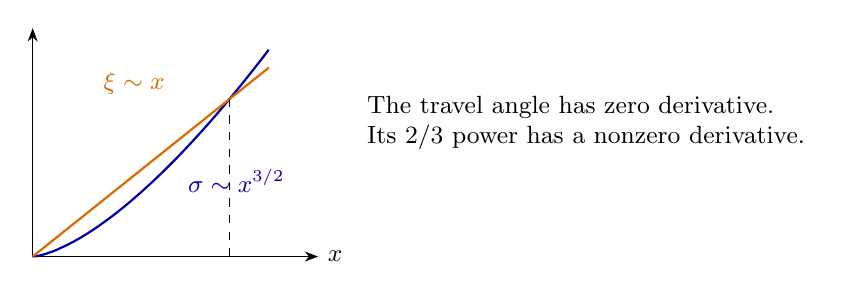
\begin{tikzpicture}[x=2.5cm,y=2.0cm,font=\small,>=Stealth]
\draw[->] (0,0)--(1.45,0) node[right] {$x$};
\draw[->] (0,0)--(0,1.45);
\draw[thick,blue!65!black] plot[domain=0:1.2,samples=50] (\x,{pow(\x,1.5)});
\draw[thick,orange!85!black] (0,0)--(1.2,1.2);
\node[blue!65!black,anchor=west] at (.74,.48) {$\sigma\sim x^{3/2}$};
\node[orange!85!black,anchor=east] at (.72,1.1) {$\xi\sim x$};
\draw[dashed] (1,0)--(1,1);
\node[align=left,anchor=west] at (1.65,.85)
 {The travel angle has zero derivative.\\
  Its $2/3$ power has a nonzero derivative.};
\end{tikzpicture}
\caption{Regularization at a turning circle. The graph displays the
leading powers with unit coefficients. The positive coefficient of
$x$ in $\xi$ is controlled uniformly at every turning circle.}
\label{fig:root-regularization}
\end{figure}

Write $\Psi_i=(\xi_i,\varphi)$ and
$\alpha_i=(\delta\circ\Psi_i^{-1})/\sqrt{\xi_i}$.
The factor is smooth and positive, also at the root, since
\[
 \alpha_i=\frac{a|\det D\Psi_i|}{U_\theta V_\theta}.
\]
For $u=(h_iW_i)\circ\Psi_i$, $h_i=\alpha_i^{-1/2}$, the equation is
\begin{equation}\label{eq:fixed-strip-airy-equation}
 \begin{split}
 (\partial_{\xi_i}^2-\xi_i\partial_\varphi^2+V_i)W_i&=F_i,\\
 V_i&=-\alpha_i^{-1/2}
       (\partial_{\xi_i}^2-\xi_i\partial_\varphi^2)\alpha_i^{1/2},\\
 F_i&=h_i((f/|\det D\Psi_i|)\circ\Psi_i^{-1}).
 \end{split}
\end{equation}
Indeed the density in these coordinates is
$\alpha_i\operatorname{diag}(1,-\xi_i)$; the positive conjugation
cancels its first derivatives. The source formula preserves
$\int uf\,dr\,d\theta=\int W_iF_i\,d\xi_i\,d\varphi$.

The middle value is $\xi_c=(3T/4)^{2/3}$. There
$\alpha_L=\alpha_R$ and
$\partial_\sigma\log\alpha_R-\partial_\sigma\log\alpha_L
=\xi_c^{-3/2}$. Consequently value and conormal matching become
\begin{equation}\label{eq:fixed-strip-cut}
 \binom{W_R}{(W_R)_{\xi_R}}
 =\begin{pmatrix}1&0\\-1/(2\xi_c)&-1\end{pmatrix}
       \binom{W_L}{(W_L)_{\xi_L}}.
\end{equation}
This matrix is independent of the state. At a type root, with boundary
chart $h_{\mathrm{bd}}$, the physical pair is
\begin{equation}\label{eq:fixed-strip-root-pair}
 u=(h_iW_i)(0,h_{\mathrm{bd}}),\qquad
 p_{\mathrm{in}}=\frac{h_{\mathrm{bd}}'}{h_i(0,h_{\mathrm{bd}})}
       (\partial_{\xi_i}W_i+\partial_{\xi_i}\log h_i\,W_i)
                                             (0,h_{\mathrm{bd}}).
\end{equation}
The tangential shear cancels because $a\varphi_r+b\varphi_\theta=0$
at the root. This identity keeps the zero mode and the full Green
pairing, not just the principal characteristics.

For completeness, all reference coordinate reciprocals used here have
the promised bounds. At a root
\[
 \xi=x\left[\tfrac32\int_0^1\sqrt t\,c_i(xt)\,dt\right]^{2/3}.
\]
Outside its collar the Morse potential has a lower bound $cA_n^{24}$;
the upper and lower bounds for $v$ then bound
$|\xi_r|=v_0/\sqrt\xi$ above and below by powers of $A_n$.
Also $\xi_c\asymp A_n^{1/3}$. Differentiating these formulas and
the inverse identity gives $\mathcal E_n^{C_s}$ bounds for charts,
inverses, $\alpha_i=w_*|\xi_r|$, $h_i$, potentials and source
factors. The perturbed bounds follow from the flow and inverse
argument in Proposition~\ref{prop:uniform-physical-geometry}.

\subsection{Crossing the positive components}

On a positive component continue the signed root coordinate and put
$y_i=-\xi_i$. Build a radial reference coordinate $y\in[0,1]$
equal to $y_L$ near the left root and $1-y_R$ near the right.
This can be done explicitly by choosing positive $y_r$ with integral
one: use the prescribed derivatives on disjoint root collars and a
positive constant on their complement, with cutoff interpolation.
The collars have total prescribed coordinate increment less than
$1/4$, so that constant and its reciprocal are bounded by
$\mathcal E_m^C$. Interpolate the logarithms of the two root height
factors, choosing height factor one in the middle. All reference
coordinate, height and source factors retain the same jet bounds.

For a perturbed state extend the \emph{differences} of the negative
coordinate jets through degree four and of the logarithmic height
jets through degree three, using cutoff Taylor polynomials. This
leaves the reference map unchanged on a compact interval $J_*$
containing the second-mode normalization and metric control.
Relative closeness of the differential gives a global diffeomorphism:
it is proper, locally invertible, and of boundary degree one.
The map and its inverse have the estimates already proved.

Writing the positive height factor in physical coordinates as
$h_{\mathbf x}$ and its chart as $\Psi_{\mathbf x}$, the positive
canonical equation for $-\widehat Lu=F_{\rm ph}$ is
\begin{equation}\label{eq:pp-fixed-canonical-source}
 P_{\mathbf x}U
 =-\left(\frac{h_{\mathbf x}}{|J_{\mathbf x}|}
       \widehat L[h_{\mathbf x}(U\circ\Psi_{\mathbf x})]\right)
             \circ\Psi_{\mathbf x}^{-1},\qquad
 F=\left(\frac{h_{\mathbf x}F_{\rm ph}}{|J_{\mathbf x}|}\right)
             \circ\Psi_{\mathbf x}^{-1}.
\end{equation}
These formulas again preserve the pairing. The continued negative
principal part is $-\partial_{y_i}^2-y_i\partial_\varphi^2$.
The specified jets match principal densities through order two.
Thus, with $d=y(1-y)$,
\begin{equation}\label{eq:readable-positive-difference}
 P_{\mathbf x}-P_*=-\partial_a(d^3e_{\mathbf x}^{ab}\partial_b)
                           +\delta V_{\mathbf x}.
\end{equation}
There is no boundary condition on the potential. Division by $d^3$
has a fixed cost: if $F,F',F''$ vanish at zero, then
\[
 F(y)/y^3=\tfrac12\int_0^1(1-t)^2F'''(ty)\,dt.
\]
Each further derivative differentiates the integrand; the $L^2$
rescaling factor $t^{-1/2}$ is integrable. The right end is identical.
This verifies the final divided-coefficient assertion of the uniform
geometric calculus. All operations use at most two height derivatives,
one root divided difference, four boundary jets, three divisions and
fixed trace and embedding costs; their sum fixes $d_*$.

The reference positive operator is
\[
 P_*=-\partial_y(a\partial_y)-c\partial_\varphi^2+V,
 \qquad a=h_*^2w_*y_r,\quad c=\frac{h_*^2w_*'}{ry_r}.
\]
It obeys $a\ge\mathcal E_m^{-C}$ and
$c\ge\mathcal E_m^{-C}d$, with all fixed coefficient jets bounded
by $\mathcal E_m^{C_s}$. Near a root it is exactly $a=1,c=y_i$;
on the rest this follows from the positive-model and transition lower
bounds for $w_*'/w_*$. These are the coefficients of the next energy
estimate.

At a type root the adjacent charts and height factors have the same
value and first physical derivative. Formula~\eqref{eq:fixed-strip-root-pair}
therefore becomes equality of canonical values and opposite inward
derivatives. Together with \eqref{eq:fixed-strip-cut} this is one
fixed transmission domain. Its smooth members really are smooth in
the original variables: the value matches tangential derivatives,
the conormal matches the first normal derivative, and the equation
solves for $a u_{rr}$ since $a>0$. Repeated normal differentiation
then matches every higher jet. This observation is what permits us
to use a common closed operator domain in the next section.

\section{Inverting on one common domain}
\label{sec:stable-inverse}
\label{sec:grn-fixed-phase-green}

A tame estimate with derivative loss is not a bounded inverse on a
single Banach space. It cannot by itself justify a Neumann series.
We first identify a source space on which the \emph{relative}
operator is bounded. The extra endpoint factor in its coefficients
will compensate for the coefficient-weight loss of the reference
inverse. Only after that Banach-space inversion do we recover all
derivatives. This order of argument keeps one neighborhood for the
entire nonlinear problem.

\subsection{Sources, scalars and the domain}

Use the canonical cylinders of Section~\ref{sec:fixed-geometry} and
retain the physical sign of the equation: on a positive cylinder its
canonical operator is $-P_{\mathbf x}$. Let $h_{\mathbf x}$ denote the
height factor in physical coordinates, $\Psi_{\mathbf x}$ the chart,
and $J_{\mathbf x}$ its Jacobian. Define
\[
 \mathscr C_{\mathbf x}u=(u/h_{\mathbf x})\circ\Psi_{\mathbf x}^{-1},
 \qquad
 \mathscr S_{\mathbf x}f=(h_{\mathbf x}f/|J_{\mathbf x}|)
                                      \circ\Psi_{\mathbf x}^{-1},
 \qquad
 \mathbb L_{\mathbf x}=
 \mathscr S_{\mathbf x}\widehat L_{\mathbf x}\mathscr C_{\mathbf x}^{-1}.
\]
These preserve the pairing with $dr\,d\theta$. For real $t$ and
angular order $s\ge0$ use the volume-source norms
\begin{equation}\label{eq:vol-source-spaces}
 \|F\|_{t,s}^2
 =\sum_m M_m^{2t}H_m^{-2\beta}
                  \|F_m\|_{L^2_{\mathrm{rad}}H^s_\varphi}^2,
 \qquad F\in\mathbb V_{t,s}.
\end{equation}
The index includes the two halves of every negative component and
the positive components. No matching or integral condition is imposed
on these sources. For inverse outputs, the corresponding volume norm is supplemented
by the absolute values of the three scalar unknowns introduced below;
these scalar coordinates are assigned to the finite middle.

The charts agree with the reference on $J_*$, so the second-mode
normalization has the fixed form $\ell_*^c W$.
Choose a compact radial $\psi$ in $J_*$ with $\mathsf Q\psi=1$ and
put $c_* =\mathscr S_*\psi=\mathscr S_{\mathbf x}\psi$.
A physical height is represented by
\[
 \eta=\mathscr C_{\mathbf x}^{-1}W+a_L\chi_L,\qquad
 \ell_*^cW=0.
\]
Its left endpoint constant is $a_L$; the right one is zero. Define
\[
 k_{\mathbf x}=D_\nu\mathcal F_q(w,u),\quad
 k_{\mathbf x}^c=\mathscr S_{\mathbf x}k_{\mathbf x},\quad
 s_{\mathbf x}=\mathscr S_{\mathbf x}\widehat L_{\mathbf x}\chi_L.
\]
Here $D_\nu$ differentiates the true residual with $u,q$ fixed,
including both its metric and reference height. The augmented operator is
\begin{equation}\label{eq:vol-abstract-complete-operator}
 \mathbb P_{\mathbf x}(W,a_L,\mu,\lambda)
 =\mathbb L_{\mathbf x}W+a_Ls_{\mathbf x}
                       +\mu k_{\mathbf x}^c+\lambda c_*.
\end{equation}
The parameter $\mu$ removes the second-mode obstruction. The additional
$\lambda$ removes the integral obstruction for arbitrary sources;
it will disappear for the original compatible problem.

At the reference let $\mathfrak g_* =\mathscr C_*1$ and
$\mathsf Q_*F=\langle\mathfrak g_*,F\rangle$.
The coefficient bounds make this continuous and
$\mathsf Q_*c_*=1$. Set $\lambda=\mathsf Q_*F$ and apply the
compatible reference inverse to $F-\lambda c_*$. This constructs a
two-sided augmented inverse $\mathbb G_*$.
In the zero angular mode the construction can be seen directly:
with $f_* =\mathscr S_*^{-1}F$,
\[
 p_0(r)=\int_{r_-}^r(\av{f_*}-\lambda\psi)(t)\,dt,
 \qquad
 u_0(r)=-\int_r^{r_+}\frac{p_0(t)}{w_*(t)}\,dt.
\]
The first integrand has total integral zero. At either endpoint use
the primitive starting there; division by $w_*$ costs a coefficient
factor, not an endpoint exponent. Subtract the left endpoint value
times $\chi_L$. This yields the required field, endpoint scalar and
normalization. It also proves uniqueness in the zero mode.

\subsection{Why two endpoint exponents are needed}

The reference construction gives one natural endpoint inverse for
every exponent in a compact subinterval of $(0,1)$
(Lemma~\ref{lem:radial-uniform-exponents}). Choose
$0<\epsilon<\min(\beta,1-\beta)$.
The inverses at $\beta-\epsilon$ and $\beta+\epsilon$ agree on compact
smooth sources: their difference satisfies the homogeneous equation,
the normalization and the natural endpoint conditions. The reference
uniqueness, together with the zero-mode formula above, makes it zero.
Hence both estimates apply to the same $\mathbb G_*$.

\begin{lemma}[A fixed coefficient loss]
\label{lem:two-weights-closed-domain}
For a fixed $L$, every real $t$ and every $s\ge0$,
\begin{equation}\label{eq:reference-negative-material-extension}
 \|\mathbb G_*F\|^{\mathrm{vol}}_{t-L,s}
                       \le C_{t,s}\|F\|_{t,s}.
\end{equation}
The first normal derivative has the same bound with at most one
additional angular source derivative. For a fixed $b\ge2$,
\begin{equation}\label{eq:fixed-base-graph-domain}
 \mathbb D_*:=\mathbb G_*(\mathbb V_{0,b}),\qquad
 \|v\|_{\mathbb D_*}=\|\mathbb P_*v\|_{0,b}
\end{equation}
is a complete closed graph domain. It includes every smooth admissible
field with the stated transmissions, endpoint conditions and slice,
whose reference source belongs to $\mathbb V_{0,b}$.
\end{lemma}

\begin{proof}
Write $\bar S_m=S_m-S_N$ on the tails and $\bar S_m=0$ on the
finite middle. Let $\pi_k,\iota_m$ be restriction to an output piece
and extension of a source on a piece by zero. The reference estimate
at exponent $\gamma$ gives
\[
 \|\pi_k\mathbb G_*\iota_m\|_{s\to s}
 \le C_s\mathcal E_k^{C_s}\mathcal E_m^{C_s}
                        e^{-\gamma(\bar S_k-\bar S_m)}.
\]
Conjugate by the $\beta$ weight. Choose $\gamma=\beta+\epsilon$
when $\bar S_k\ge\bar S_m$ and $\gamma=\beta-\epsilon$ otherwise.
The resulting block $K_{km}$ satisfies
\begin{equation}\label{eq:global-two-weight-block-bound}
 \|K_{km}\|_{s\to s}
 \le C_s\mathcal E_k^{C_s}\mathcal E_m^{C_s}
                    e^{-\epsilon|\bar S_k-\bar S_m|}.
\end{equation}
There is no angular-order loss in this volume estimate. The first
normal estimate of the radial construction adds at most one angular
derivative and otherwise has the same block argument.

For each $\delta>0$ the enlarged weight satisfies
\[
 |\log M_k-\log M_m|
 \le\delta|\bar S_k-\bar S_m|+C_\delta.
\]
This follows from the derivative of
$n^{5/2}\log^2(e+n)$ with respect to $2n^3/3$ tending to zero.
Using $\mathcal E^{C_s}\le C_sM$, we find, for $L\ge2$,
\[
 M_k^{t-L}\|K_{km}\|M_m^{-t}
 \le C_sM_k^{2-L}(M_k/M_m)^{t-1}
                         e^{-\epsilon|\bar S_k-\bar S_m|}
 \le C_{t,s}e^{-(\epsilon/2)|\bar S_k-\bar S_m|}.
\]
Choose $\delta$ so that $|t-1|\delta\le\epsilon/2$.
The last matrix has bounded row and column sums: the $S_n$ are
uniformly separated and there are only finitely many pieces at each
index. The $\ell^2$ Schur estimate proves
\eqref{eq:reference-negative-material-extension}.

The definition of $\mathbb D_*$ makes it complete. Approximate a
source by compact smooth sources. The estimate gives local volume
convergence and the equation passes to distributions, with weak
transmissions. If $v_j\to v$ in the ambient volume space and
$\mathbb P_*v_j\to F$ in the source space, then
$v_j=\mathbb G_*\mathbb P_*v_j\to\mathbb G_*F$, so
$v=\mathbb G_*F$; the graph is closed. First-normal estimates identify
the local weak traces. Finally, any smooth admissible $y$ with source
$F$ differs from $\mathbb G_*F$ by a homogeneous normalized natural
endpoint solution, hence is equal to it. This proves the stated
exhaustion of admissible smooth fields.
\end{proof}

\begin{figure}[htbp]
\centering
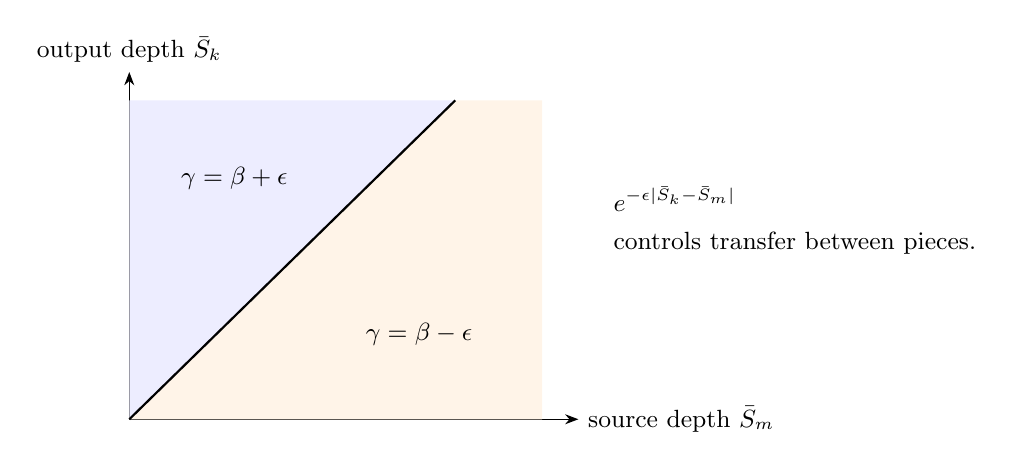
\begin{tikzpicture}[x=.92cm,y=.9cm,font=\small,>=Stealth]
\draw[->] (0,0)--(6.2,0) node[right] {source depth $\bar S_m$};
\draw[->] (0,0)--(0,4.9) node[above] {output depth $\bar S_k$};
\fill[blue!7] (0,0)--(4.5,4.5)--(0,4.5)--cycle;
\fill[orange!9] (0,0)--(5.7,0)--(5.7,4.5)--(4.5,4.5)--cycle;
\draw[thick] (0,0)--(4.5,4.5);
\node at (1.45,3.4) {$\gamma=\beta+\epsilon$};
\node at (4,1.2) {$\gamma=\beta-\epsilon$};
\node[align=left,anchor=west] at (6.55,2.8)
 {$e^{-\epsilon|\bar S_k-\bar S_m|}$\\[3pt]
  controls transfer between pieces.};
\end{tikzpicture}
\caption{The same reference inverse is estimated with two endpoint
weights. Each weight is used on one side of the diagonal. Their minimum
gives decay in the distance between source and output depths.}
\label{fig:two-weights}
\end{figure}

\subsection{The estimate that explains cubic matching}

On a normalized positive cylinder consider
\[
 P_ju=-(au')'+j^2cu+Vu=F,
 \qquad a\ge\mathcal E_m^{-C},\quad
 c\ge\mathcal E_m^{-C}d,\quad d=y(1-y).
\]
Coefficient derivatives through order two, and $a^{-1}$, are bounded
by $\mathcal E_m^{C_1}$. Boundary values are arbitrary. We claim
\begin{equation}\label{eq:vol-arbitrary-boundary-graph-bound}
 \begin{split}
 &\|du'\|_2+\|\av j d^{3/2}u\|_2+\|d^2u''\|_2
   +\|\av j^2d^3u\|_2+\|\av j d^{5/2}u'\|_2\\
 &\hspace{30mm}\le\mathcal E_m^C(\|F\|_2+\|u\|_2),
 \end{split}
\end{equation}
where $\av j=(1+j^2)^{1/2}$ in this display.
For fixed $j$, a distributional $L^2$ solution with $F\in L^2$
is $H^2$ up to the endpoints by the regular ordinary differential
equation. Uniform bounds come from the following calculation, not
from that preliminary regularity statement.

Multiply by $d^2\bar u$ and integrate. Since $d=0$ at the ends,
\[
 \int a|(du)'|^2+j^2\int cd^2|u|^2
 =\operatorname{Re}\langle F,d^2u\rangle
       +\int a|d'|^2|u|^2-\int Vd^2|u|^2.
\]
This bounds $du'$ and $jd^{3/2}u$. Now put $v=d^2u$; it has
zero trace and
\[
 P_jv=d^2F-2a(d^2)'u'-(a(d^2)')'u.
\]
The right side is controlled by the first estimate. With $q_0=c/a$,
the same is true of $F_1=-v''+j^2q_0v$. Squaring and integrating
the cross term twice gives
\[
 \|v''\|_2^2+j^4\|q_0v\|_2^2+2j^2\int q_0|v'|^2
 =\|F_1\|_2^2+j^2\int q_0''|v|^2.
\]
The final integral is controlled because $d^4\le Cd^3$.
Use $q_0\ge\mathcal E_m^{-C}d$ and expand $v',v''$ to obtain
\eqref{eq:vol-arbitrary-boundary-graph-bound}.

Every second-order term in the perturbation
\eqref{eq:readable-positive-difference} is now controlled:
$d^3u_{yy}$ by $d^2u''$, $d^3u_{y\varphi}$ by
$\av j d^{5/2}u'$, and $d^3u_{\varphi\varphi}$ by
$\av j^2d^3u$. A derivative on the coefficient leaves only terms
controlled by the first two norms. Fourier convolution in $\varphi$
therefore gives, for $s\ge b$,
\begin{equation}\label{eq:readable-positive-relative-bound}
 \|\delta P_{\mathbf x}u\|_s
 \le C_sH_m^\beta\mathcal E_m^{C_s}
 \left[\mathfrak n_{b_0,m}(\|F\|_s+\|u\|_s)
       +\mathfrak n_{s+d_*,m}(\|F\|_b+\|u\|_b)\right].
\end{equation}
This is the reason for matching the principal density to order two.
It controls a second-order perturbation without imposing artificial
boundary conditions on the reference solution.

We also use an elementary first-normal estimate on every normalized
piece. Its radial equation has the form
$Au''+Bu'+(j^2C+D_0)u=F$ with $A$ bounded away from zero and all
coefficients bounded by fixed powers of $\mathcal E_m$.
The equation and
$\|u'\|_2^2\le C\|u\|_2(\|u''\|_2+\|u\|_2)$ give
\begin{equation}\label{eq:vol-reference-first-normal-bound}
 \|u'\|_2\le\mathcal E_m^C(\|F\|_2+\av j\|u\|_2),
 \qquad
 \|u''\|_2\le\mathcal E_m^C(\|F\|_2+\av j^2\|u\|_2).
\end{equation}
Young's inequality absorbs the intermediate $u'$ term. Density
extends the estimates to volume solutions. Neither estimate assumes
zero boundary data.

\subsection{The bounded relative operator}

Define on compact smooth sources
\[
 \mathscr R_{\mathbf x}=(\mathbb P_{\mathbf x}-\mathbb P_*)\mathbb G_*.
\]
If $\mathbb G_*F=(W,a_L,\mu,\lambda)$, then
\begin{equation}\label{eq:vol-normalized-relative-identity}
 \mathscr R_{\mathbf x}F
 =\delta\mathbb L_{\mathbf x}W
      +a_L(s_{\mathbf x}-s_*)+\mu(k_{\mathbf x}^c-k_*^c).
\end{equation}
The last scalar has no difference. On a negative piece only the
canonical potential varies. On a positive piece use
\eqref{eq:readable-positive-relative-bound}, putting its compact scalar
sources into $F$. Every coefficient difference at the output piece
$k$ contains $H_k^\beta$.

Here is the actual base-space calculation. Combine that factor with
\eqref{eq:global-two-weight-block-bound}. For low coefficients the
norm of the block from $m$ to $k$ is bounded by
\begin{equation}\label{eq:rewrite-relative-block}
 C\mathfrak n_{b_0}\,M_k^CM_m^C
            e^{-\beta\bar S_k-\epsilon|\bar S_k-\bar S_m|}.
\end{equation}
For every fixed $C$ and $\delta>0$,
$M_j^C\le C_\delta e^{\delta\bar S_j}$, while
$\bar S_m\le\bar S_k+|\bar S_k-\bar S_m|$.
Choose $\delta<\min(\beta/4,\epsilon/2)$. The matrix in
\eqref{eq:rewrite-relative-block} is bounded by
\[
 C'\mathfrak n_{b_0}
       e^{-(\beta/2)\bar S_k-(\epsilon/2)|\bar S_k-\bar S_m|}.
\]
Its row and column sums are uniformly bounded. Thus
\begin{equation}\label{eq:rewrite-base-relative}
 \|\mathscr R_{\mathbf x}\|_{\mathbb V_{0,b}\to\mathbb V_{0,b}}
                         \le C\mathfrak n_{b_0}<\tfrac12
\end{equation}
after increasing $b_0$ to cover the finite low derivatives and
then decreasing $\epsilon_0$. This is a bounded operator on precisely
one source space; no identification of a derivative-losing inverse
with a bounded endomorphism has been made.

For higher orders keep one coefficient factor at high order in the
product estimate. The same summation proves, for $t\ge0$, $s\ge b$,
\begin{equation}\label{eq:compact-volume-relative-bound}
 \begin{split}
 \|\mathscr R_{\mathbf x}F\|_{t,s}
 +\|[\Lambda,\mathscr R_{\mathbf x}]F\|_{t,s}
 \le C_{t,s}\bigl[\epsilon_0\|F\|_{0,s}
             +\mathfrak n_{t+s+d_*}\|F\|_{0,b}\bigr],
 \end{split}
\end{equation}
where $\Lambda=|D_\varphi|$. Assign frequency zero to $a_L,\lambda$
and frequency two to $\mu$. For multiplication by a coefficient,
the commutator Fourier matrix gains $|k|-|j|$, bounded by $|k-j|$;
one additional coefficient derivative therefore proves the same bound.
The scalar commutators are retained:
$\Lambda(s_{\mathbf x}-s_*)a_L$ and
$(\Lambda-2)(k_{\mathbf x}^c-k_*^c)\mu$.

Approximation by compact smooth sources identifies this extension
with the differential difference in distributions on $\mathbb D_*$.
The canonical transmissions are fixed, hence
\begin{equation}\label{eq:current-fixed-domain-factorization}
 \mathbb P_{\mathbf x}=(I+\mathscr R_{\mathbf x})\mathbb P_*
                         \quad\text{on }\mathbb D_*.
\end{equation}
This is the desired comparison on a common domain.

\subsection{Higher derivatives from the one base inverse}

By \eqref{eq:rewrite-base-relative}, set
\[
 \widetilde F=(I+\mathscr R_{\mathbf x})^{-1}F,
 \qquad v=\mathbb G_*\widetilde F.
\]
The inverse in the first formula is taken only on $\mathbb V_{0,b}$.
We now explain why this same solution has all the required regularity.

First recover angular derivatives. If $C=[\Lambda,\mathscr R]$, then
for $U_\delta=e^{i\delta\Lambda}$,
\[
 [U_\delta,\mathscr R]
 =i\int_0^\delta U_{\delta-t}CU_t\,dt.
\]
Apply this to $(I+\mathscr R)\widetilde F=F$. The base inverse
bounds the difference quotients of $\widetilde F$ whenever those
of $F$ are bounded. Fatou's lemma on Fourier coefficients gives the
first derivative; iteration gives all integer orders. Quantitatively,
the commuted equation at order $N$ contains
$\sum_{k=0}^{N-1}\Lambda^kC\Lambda^{N-1-k}\widetilde F$.
Interpolate the bound for $C$ at the base and at order $N-1$, treating
the high coefficient size as a weight in the source Hilbert norm.
Each term is then bounded by
\[
 C_N\bigl(\|\widetilde F\|_{N-1}
 +(1+\mathfrak n_{N+d_*})\|\widetilde F\|_b\bigr).
\]
Interpolation and Young's inequality absorb the first term into
half the order-$N$ norm plus a base norm. This proves the one-high-factor
estimate without smallness of high coefficient norms. Real orders
follow by Hilbert interpolation, or may be replaced by their ceilings.

Next use the already solved identity
$\widetilde F=F-\mathscr R_{\mathbf x}\widetilde F$.
Estimate its last term by \eqref{eq:compact-volume-relative-bound}.
It belongs to every coefficient-weight order once angular regularity
is known. Thus
\begin{equation}\label{eq:full-source-tame-resolvent}
 \|\widetilde F\|_{t,s}
 \le C_{t,s}\bigl[\|F\|_{t,s}
       +(1+\mathfrak n_{t+s+d_*})\|F\|_{0,b}\bigr].
\end{equation}
No second inversion is required.

\paragraph{The normal recursion uses the original source.}
Estimate \eqref{eq:full-source-tame-resolvent} controls angular
derivatives of $\widetilde F$. We do not assume normal derivatives
of that corrected source. Use instead the current equation
$\mathbb P_{\mathbf x}v=F$, and subtract its three scalar columns:
\[
 F^\circ=F-a_Ls_{\mathbf x}-\mu k_{\mathbf x}^c-\lambda c_*.
\]
Rescale each negative half to a unit radial interval, denoted by $y$;
the positive intervals already have this normalization. All rescaling
factors and their reciprocals are reference coefficient factors.
Solving the equation for its nonvanishing normal coefficient gives
\begin{equation}\label{eq:rewrite-normal-recursion-base}
 \partial_y^2W=\sum_{(i,j)\in I}A_{ij}\partial_y^i
                      \partial_\varphi^jW+B F^\circ,\qquad
 I=\{(1,1),(0,2),(1,0),(0,1),(0,0)\}.
\end{equation}
On a negative half the unscaled equation is
$W_{\xi\xi}=\xi W_{\varphi\varphi}-VW+F^\circ$.
On a positive piece the normal coefficient has a lower bound
$\mathcal E_m^{-C}$ on the common neighborhood. Thus all the
$A_{ij},B$ obey the coefficient calculus of
Proposition~\ref{prop:uniform-physical-geometry}, with a fixed
state-derivative loss $d_{\rm geo}$.

For $a\ge2$ the actual mixed recursion is
\begin{equation}\label{eq:rewrite-mixed-normal-recursion}
 \begin{split}
 \partial_y^a\partial_\varphi^b W
 ={}&\sum_{(i,j)\in I}\sum_{p=0}^{a-2}\sum_{q=0}^{b}
       \binom{a-2}{p}\binom bq
       (\partial_y^p\partial_\varphi^q A_{ij})
       \partial_y^{a-2-p+i}\partial_\varphi^{b-q+j}W\\
 &+\partial_y^{a-2}\partial_\varphi^b(BF^\circ).
 \end{split}
\end{equation}
Every field on the right has at most $a-1$ normal derivatives
and total order at most $a+b$. A derivative falling on a
coefficient lowers the remaining field order by that amount.
Consequently the expansion terminates in angular derivatives of
$W$, angular derivatives of $W_y$, and mixed derivatives of
$F^\circ$. At total order $s$ their respective orders are at most
$s$, $s-1$, and $s-2$.
Starting with the already established angular and first-normal
regularity, this identity in distributions proves the existence of
the mixed derivatives successively.

Here is the quantitative form of this recursion. Fix a base order
$b_1\ge4$, and let $\mathfrak n_{r,m}$ be the localized displacement
seminorm on the bounded-overlap neighborhoods used in
Section~\ref{sec:fixed-geometry}. For $s\ge b_1+2$ put
\[
 \mathcal A_{s,m}
 =\|W_m\|_{L_y^2H_\varphi^s}
   +\|\partial_yW_m\|_{L_y^2H_\varphi^{s-1}}
   +\|F_m^\circ\|_{H^{s-2}_{y,\varphi}}.
\]
The finite expansion of \eqref{eq:rewrite-mixed-normal-recursion}
gives
\begin{equation}\label{eq:rewrite-local-mixed-bound}
 \|W_m\|_{H^s_{y,\varphi}}
 \le C_s\mathcal E_m^{C_s}
       \left[\mathcal A_{s,m}
       +(1+\mathfrak n_{s+d_{\rm geo},m})\mathcal A_{b_1,m}\right].
\end{equation}
To justify the tame form, keep the derivative count in each
expanded term: the sum of coefficient derivative orders and the
remaining field or source order is at most $s$. Interpolate each
intermediate coefficient norm between its fixed low norm and its
order-$s+d_{\rm geo}$ norm, and each remaining field norm between
the corresponding entries of $\mathcal A_{b_1,m}$ and
$\mathcal A_{s,m}$. The interpolation exponents have sum at most
one. The weighted arithmetic--geometric mean inequality therefore
places at most one factor at high order. Sobolev embedding uses only
the fixed base order $b_1$. Reciprocal normal coefficients have the
same property by their positive lower bound. This proves
\eqref{eq:rewrite-local-mixed-bound}; it does not require smallness
of any order-$s$ state norm.

The reference factors in that finite expansion may have an exponent
$C_s$ growing with $s$. Absorb their \emph{complete product} only
after the expansion: $\mathcal E_m^{C_s}\le C_sM_m$ costs one
coefficient-weight order. Paying for each recursion separately
would obscure this fixed loss.
For precision, write
\[
 \bigl(\|Z\|_{t,s}^{\rm mix}\bigr)^2
 =\sum_m M_m^{2t}H_m^{-2\beta}
       \sum_{a+b\le s}\|\partial_y^a\partial_\varphi^b Z_m\|_2^2.
\]
The zeroth-normal entry of $\mathcal A_{s,m}$ is controlled by
\eqref{eq:reference-negative-material-extension}. For its
first-normal entry, use the first-normal reference bound at angular
order $s-1$: its one extra angular derivative asks for precisely
order $s$ of $\widetilde F$. Summing
\eqref{eq:rewrite-local-mixed-bound} therefore yields
\begin{equation}\label{eq:rewrite-global-mixed-bound}
 \begin{split}
 \|W\|_{t,s}^{\rm mix}
 \le C_{t,s}\bigl[&
   \|\widetilde F\|_{t+L+1,s}
   +\|F\|_{t+1,s-2}^{\rm mix}\\
 &+(1+\mathfrak n_{t+s+D})\|F\|_{0,b_1}^{\rm mix}\bigr].
 \end{split}
\end{equation}
Here $D$ is fixed: it covers $L+1$, $d_{\rm geo}$ and the fixed
base and embedding orders. The scalar columns are compactly
supported and satisfy the same tame estimate; their scalars are
bounded by the base inverse. In the high-coefficient term the
$M^{t+L+1}$ weight is placed on the localized state norm, leaving
the low field in the reference output space of weight $-L$.
Choose the original $b_0$ large enough to control the finitely many
base norms used here. The finitely many orders below $b_1+2$ follow
from this same base calculation.

Apply \eqref{eq:full-source-tame-resolvent} to the first term in
\eqref{eq:rewrite-global-mixed-bound}. The weight and derivative
indices there have sum $t+s+L+1$; the source term has sum $t+s-1$.
Thus taking $t+s\le r$ costs a fixed number of grading orders,
independent of $r$. The physical coordinate and source transformations
have their already proved fixed tame losses. Increasing $d_*$
once to include those losses gives \eqref{eq:readable-physical-inverse-tame}.
Physical seam jets match by the argument at the end of
Section~\ref{sec:fixed-geometry}.

Undoing the transformations gives
\[
 \widehat L_{\mathbf x}\eta+k_{\mathbf x}\mu+\lambda\psi=f,
 \qquad \ell_*\eta=0.
\]
Endpoint fluxes vanish. Moreover $\mathsf Qk_{\mathbf x}=0$ by
differentiating the integral compatibility of the original residual.
Integration therefore gives $\lambda=\mathsf Qf$. For
$f\in\mathcal Y_\beta$ it is zero.

\begin{proposition}[The perturbed scalar inverse]
\label{prop:rewrite-volume-inverse}
On the single neighborhood fixed above there is a unique normalized
pair $G_{\mathbf x}f=(\eta,\mu)$ solving
$\widehat L_{\mathbf x}\eta+k_{\mathbf x}\mu=f$ for every
$f\in\mathcal Y_\beta$. The height belongs to
$\mathcal X_\beta\cap\ker\ell_*$ and has right endpoint value zero.
Its left endpoint value is free. For a fixed $d_*$,
\begin{equation}\label{eq:readable-physical-inverse-tame}
 \|G_{\mathbf x}f\|_s
 \le C_s\bigl[\|f\|_{s+d_*}
       +(1+\mathfrak n_{s+d_*})\|f\|_{b+d_*}\bigr].
\end{equation}
The inverse is smooth tame jointly in state and source.
\end{proposition}

\begin{proof}
Existence and the estimate were proved above. Factorization on
$\mathbb D_*$ gives both inverse identities, and its exhaustion
property gives uniqueness among smooth admissible fields. The
resolvent identity first proves continuity in the base space and
then, using the higher estimates, at every stronger order. The
coefficient family is smooth tame. Hamilton's inverse-family theorem
\cite[II, Theorem~3.1.1, p.~150]{Hamilton1982} now applies: a smooth
tame linear family with unique solutions and a continuous tame inverse
has a smooth tame inverse. Its uniqueness and continuity hypotheses
have thus been checked before invoking it.
\end{proof}

\section{From the linear seed to a nonlinear height}
\label{sec:solving-the-equation}
\label{sec:exact-return-height}

We can now see why the unknowns were chosen as they were. The height
solves the curvature equation. One compact metric parameter removes
its second-mode obstruction. One radial control per negative component
adjusts the mean travel angle. Finally the odd boundary charts adjust
the nonconstant return maps. The last two tasks are separated by taking
the angular mean. Their feedback through the height contains the small
amplitude $q$, which makes the coupled linear problem invertible.

\subsection{The residual and its four unknowns}

Use the state \eqref{eq:rewrite-state}, with $q\in\R$ a parameter.
Set
\begin{equation}\label{eq:readable-joint-residual}
 \mathcal R(\mathbf x,q)=(\mathcal A,\mathfrak e),
 \qquad \mathcal A=\mathcal F_q(w,u),
 \qquad \mathfrak e=\mathfrak e(qu,\kappa,h_L).
\end{equation}
The tangent and residual spaces are
\[
 \mathfrak X=(\mathcal X_\beta\cap\ker\ell_*)\times\R
       \times\mathcal K_\beta\times\mathcal Z_{\beta,\mathrm{odd}},
 \qquad
 \mathfrak Y=\mathcal Y_\beta\times\mathcal Z_{\beta,\mathrm{even}}.
\]
The second residual space includes its angular means. The scalar
space uses the integral compatibility from the connection form.
The normalized scalar equation is smooth through $q=0$ by
\eqref{eq:normalized-integral}. The coefficient and flow calculus of
Section~\ref{sec:fixed-geometry} makes $\mathcal R$ smooth tame on
one open neighborhood $\mathfrak n_{b_0}<\epsilon_0$.
At
\[
 q=0,\qquad \mathbf x_0=(\Phi_*,0,0,\id)
\]
it is zero: $\mathscr L_{w_*}\Phi_*=0$ and the reference return maps
are the prescribed rotations.

Write the differentiated circle rows as
\begin{equation}\label{eq:joint-circle-linear-rows}
 C_{\mathbf x}^{\circ}=D_Z\mathfrak e,\quad
 R_{\mathbf x}^{\circ}=\av{C_{\mathbf x}^{\circ}},\quad
 \mathcal D_{\mathbf x}=D_\kappa\mathfrak e,\quad
 J_{\mathbf x}=\av{\mathcal D_{\mathbf x}}.
\end{equation}
The map on component $m$ depends on its height jets, its chart and
$\kappa_m$. It does not depend on $\nu$ or the endpoint scalar,
whose positive jets are supported in positive components.
Thus $J_{\mathbf x}$ is diagonal. At a radial state
$\mathfrak e=T(w)-T(w_*)$, so the normalization of the controls gives
$J_0=I$. On one small low-order neighborhood its entries are uniformly
separated from zero and its inverse is smooth tame.

The reference mean derivative annihilates nonzero height frequencies
and odd chart directions. For a radial increment $Z$ it is
\begin{equation}\label{eq:rewrite-reference-circle-row}
 (R_0^\circ Z)_m
 =-\int_{I_m}v_0\frac{1+w_*^2}{w_*}Z_r\,dr.
\end{equation}
To verify this, at a radial state the speed is
$v_0w_*\sqrt D/(w_*+Z_r)$, with
$D=1-2w_*Z_r-Z_r^2$. Its logarithmic variation is
$-(1+w_*^2)Z_r/w_*$. Angular translation invariance gives the
nonzero-mode assertion. In particular $R_0^\circ\Phi_*=0$.

With $K_{\mathbf x}=D_\kappa\mathcal A$ and
$k_{\mathbf x}=D_\nu\mathcal A$, the corrected linear equations are
\begin{equation}\label{eq:corrected-coupled-linear-system}
 \begin{split}
 \widehat L_{\mathbf x}\eta+k_{\mathbf x}\mu+K_{\mathbf x}\xi&=f,
                    \qquad \ell_*\eta=0,\\
 qC_{\mathbf x}^{\circ}\eta+\mathcal D_{\mathbf x}\xi
                            +\mathcal M_Tv&=g.
 \end{split}
\end{equation}
The actual chart variation is $v\circ h_L$. The equation differs
from the true derivative only by the two residual terms already
identified and the chart error in
\eqref{eq:full-height-chart-derivative}.

\begin{figure}[htbp]
\centering
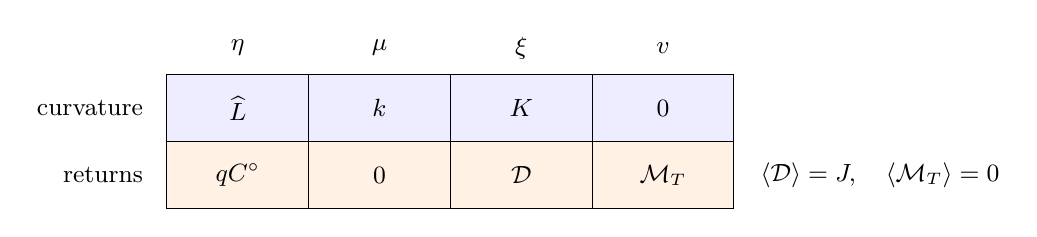
\begin{tikzpicture}[x=1.8cm,y=.85cm,font=\small]
\fill[blue!7] (0,1) rectangle (4,2);
\fill[orange!10] (0,0) rectangle (4,1);
\draw (0,0) rectangle (4,2);
\draw (0,1)--(4,1);
\foreach \x in {1,2,3} {\draw (\x,0)--(\x,2);}
\node at (.5,2.4) {$\eta$}; \node at (1.5,2.4) {$\mu$};
\node at (2.5,2.4) {$\xi$}; \node at (3.5,2.4) {$v$};
\node at (.5,1.5) {$\widehat L$}; \node at (1.5,1.5) {$k$};
\node at (2.5,1.5) {$K$}; \node at (3.5,1.5) {$0$};
\node at (.5,.5) {$qC^\circ$}; \node at (1.5,.5) {$0$};
\node at (2.5,.5) {$\mathcal D$}; \node at (3.5,.5) {$\mathcal M_T$};
\node[anchor=east] at (-.1,1.5) {curvature};
\node[anchor=east] at (-.1,.5) {returns};
\node[anchor=west] at (4.12,.5) {$\av{\mathcal D}=J,\quad\av{\mathcal M_T}=0$};
\end{tikzpicture}
\caption{The corrected derivative and the roles of its four columns.
Taking the mean of the second row removes the chart column. Feedback
from that row to the height is multiplied by $q$.}
\label{fig:coupled-columns}
\end{figure}

\subsection{The control contribution gains all component weights}

Let $G_{\mathbf x}$ be the scalar inverse of
Proposition~\ref{prop:rewrite-volume-inverse} and set
$U_{\mathbf x}=G_{\mathbf x}K_{\mathbf x}$.
The useful base space for control increments is
\[
 B_\beta=\left\{\xi:\sum_mH_m^{-2\beta}|\xi_m|^2<\infty\right\}.
\]
For every $s$, with a fixed loss $d_*$,
\begin{equation}\label{eq:weak-control-smoothing}
 \|K_{\mathbf x}\xi\|_{\mathcal Y_\beta,s}
 +\|U_{\mathbf x}\xi\|_{\mathcal X_\beta,s}\!+|(U_{\mathbf x}\xi)_{\mu}|
 \le C_s(1+\mathfrak n_{s+d_*})\|\xi\|_{B_\beta}.
\end{equation}
In the middle term the norm denotes the height component of $U\xi$.

Here is the reason for this strong smoothing in the component index.
Differentiate the removable formula for $\mathcal F_q$ with respect
to a control. Every term contains that control increment and a
positive height jet: the curvature expression is unchanged by adding
a constant to the height. This remains true at $q=0$, where the
derivative is that of $\mathscr L_wu$. On component $m$ write
$\xi_m=H_m^\beta b_m$. The height jet contributes another
$H_m^\beta$. After dividing by the source weight there remains a
factor $H_m^\beta$, which absorbs every fixed power of $M_m$ and
every complete coefficient product. The endpoint scalar has no
height jet on these control supports. The local product bound puts
one state factor at high order, and summation of $|b_m|^2$ gives the
estimate for $K$. Composing with $G$ adds only its fixed loss.

\subsection{Solving the coupled equations}

Put $g_0=\av g$. Solving the first row of
\eqref{eq:corrected-coupled-linear-system} gives
$y=(\eta,\mu)=Gf-U\xi$. Taking the mean of the second then gives
\[
 (I-qJ^{-1}R^\circ U)\xi
              =J^{-1}(g_0-qR^\circ Gf).
\]
The rows act on the height component of $G$ and $U$.
By \eqref{eq:weak-control-smoothing}, $R^\circ U$ is bounded on
the \emph{same} $B_\beta$, with a constant controlled by finitely
many state norms. Choose the low neighborhood to control those norms,
then choose $|q|$ so that
$\|qJ^{-1}R^\circ U\|_{B_\beta\to B_\beta}<1/2$.
The solution is therefore
\begin{equation}\label{eq:joint-height-circle-inverse}
 \begin{split}
 \xi&=(I-qJ^{-1}R^\circ U)^{-1}J^{-1}(g_0-qR^\circ Gf),\\
 (\eta,\mu)&=Gf-U\xi,\\
 v&=\mathcal M_T^{-1}(g-qC^\circ\eta-\mathcal D\xi).
 \end{split}
\end{equation}
The last argument has zero mean by the first equation, so the inverse
in \eqref{eq:rewrite-circle-inverse} applies.

Higher control norms come from the already solved identity
\[
 \xi=J^{-1}(g_0-qR^\circ Gf)+qJ^{-1}R^\circ U\xi.
\]
The final term has every higher norm using only
$\|\xi\|_{B_\beta}$ and one high state norm, by the smoothing
estimate. The first has the requisite source norms with fixed loss.
Consequently the same solution lies in all control spaces, with a
tame bound. Substitution gives the height and chart estimates.
The resolvent identity proves base continuity; this identity and its
higher estimates prove continuity in every order. Hamilton's
inverse-family theorem applies to the control inverse, making all
three formulas smooth tame. Thus
\[
 V(\mathbf x,q)(f,g)=(\eta,\mu,\xi,v\circ h_L)
\]
is a smooth tame map, linear in the residual pair.

\subsection{The exact quadratic-error identity}

We invoke Hamilton's implicit theorem with quadratic error
\cite[III, Theorem~3.3.1, pp.~211--212]{Hamilton1982}.
In the notation here its hypothesis is a smooth tame $\mathcal R$
on an open subset of tame spaces, together with a linear smooth tame
$V$ and a bilinear smooth tame $\mathcal Q$ such that
\begin{equation}\label{eq:rewrite-hamilton-hypothesis}
 D_{\mathbf x}\mathcal R\,V y
                  =y+\mathcal Q(\mathbf x,q)[\mathcal R,y].
\end{equation}
At an initial zero this gives a local smooth tame solution branch in
the parameter. We check the identity with two \emph{independent}
residual arguments; an informal quadratic bound would not suffice.

For the increments in \eqref{eq:joint-height-circle-inverse}, the
actual derivative is
\begin{equation}\label{eq:joint-height-circle-quadratic-error}
 D_{\mathbf x}\mathcal R(\eta,\mu,\xi,v\circ h_L)
 =\bigl(f+q\partial_\theta(B\mathcal A\eta_\theta)
              +\mathscr E_{\mathbf x}(\mathfrak e)\eta,
        \ g+\mathcal Q_h(\mathfrak e,v)\bigr).
\end{equation}
For $r=(r_1,r_2)$ and $y=(f,g)$ define
\[
 \mathcal Q(\mathbf x,q)[r,y]
 =\bigl(q\partial_\theta(Br_1\eta_\theta)
                   +\mathscr E_{\mathbf x}(r_2)\eta,
              \mathcal Q_h(r_2,v)\bigr).
\]
In $\mathcal Q_h$ keep the actual state paths in
\eqref{eq:full-height-chart-derivative}, replacing only its explicit
$\mathfrak e,\mathfrak e'$ factors by $r_2,r_2'$.
The same convention was built into $\mathscr E$.
The increments are linear in $y$, so this formula is bilinear in
$(r,y)$ and gives \eqref{eq:rewrite-hamilton-hypothesis}.

Its scalar component has zero integral: one term is an angular
derivative and the other is an interior divergence with flat global
endpoint flux. The parity of its circle component is the required
one. Each product has two weak endpoint factors; the coefficient
calculus and flow estimates from Section~\ref{sec:fixed-geometry}
therefore make $\mathcal Q$ smooth tame into $\mathfrak Y$.
All state neighborhoods in this argument are controlled by one fixed
finite order. No output order changes their radius.

The remaining hypotheses have already been verified: the spaces and
the normalization slice are tame direct summands; the domain is open;
the residual is smooth tame; $V$ is smooth tame; and the reference
state is a zero. At a zero the identity itself implies surjectivity
of the state derivative. Hamilton's theorem gives a single smooth
branch
\begin{equation}\label{eq:rewrite-weak-branch}
 \mathbf x(q)=(u_q,\nu_q,\kappa_q,h_{L,q}),\qquad
 \mathcal R(\mathbf x(q),q)=0,\qquad
 u_q=\Phi_*+O(q)\quad\text{in every }\mathcal X_\beta\text{ norm}.
\end{equation}
This solves the nonlinear system in the weak endpoint scale. The
following section extracts stronger information from the equations
themselves, rather than starting another iteration in another space.

\section{The endpoint gain and the closed surface}
\label{sec:final-proof}

The nonlinear construction used the weak weight $H^\beta$ because
the reference inverse is available for exponents below one. The
metric controls nevertheless acquire twice that exponent. This is
forced by two angular average equations. The first recovers the mean
height from a quadratic expression; the second recovers the metric
controls from that mean and another quadratic expression. There is
no new nonlinear iteration in a stronger function space.
Every height in $\mathcal X_\beta$ already has a smooth flat endpoint
extension. The gain below strengthens the annular result by
quantifying the corrections to the mean height and the metric;
geometric closure uses the flat extensions established in
Section~\ref{sec:fixed-geometry}.

\subsection{The two identities that improve decay}

Let $\mathfrak F_w(U)$ be the connection period from
\eqref{eq:cart-mean-path-flux}. Its derivative at $U=0$ is
$w\av{U_r}$. Write its bilinear Taylor remainder as
\begin{equation}\label{eq:posterior-period-bilinear}
 \mathcal B_{w,U}(v_1,v_2)
 =\int_0^1(1-t)D_U^2\mathfrak F_w(tU)[v_1,v_2]\,dt.
\end{equation}
The normalized period of a solution vanishes, because its radial
derivative is the mean scalar residual and its endpoint value is
zero. Therefore, with $u^{\rm av}=\av u$,
\begin{equation}\label{eq:mean-recovered-derivative}
 (u^{\rm av})'=-q w^{-1}\mathcal B_{w,qu}(u,u).
\end{equation}

For the mean circle map use additive coordinates
$\mathbf v=(Z,\kappa,a)$, where $Z=qu$ and $h_L=\id+a$, and put
\[
 \mathcal C(\mathbf v)=\av{\mathfrak e(\mathbf v)},
 \qquad
 \mathcal B^\circ_{\mathbf v}(v_1,v_2)
 =\int_0^1(1-t)D^2\mathcal C(t\mathbf v)[v_1,v_2]\,dt.
\]
Its first derivative is the identity on $\kappa$, zero on odd chart
directions, and $R_0^\circ$ on the radial mean height. Thus the
second identity at a solution is
\begin{equation}\label{eq:weak-posterior-control}
 0=\kappa+qR_0^\circ u^{\rm av}
                       +\mathcal B^\circ_{\mathbf v}(\mathbf v,\mathbf v).
\end{equation}
The two displayed formulas already explain the exponent $2\beta$.
We must verify these estimates in the stronger topology, including
parameter derivatives, to retain this quantitative conclusion for
the entire branch.

\subsection{Two weak factors give one strong remainder}

Choose a convex neighborhood of the raw state
$(U,\nu,\kappa,a)=(0,0,0,0)$ in the weak product spaces, small in
one finite norm. On it the denominators $D,Q/w$ are positive and
the circle lifts are uniformly increasing. Both Taylor segments
above stay in this neighborhood; the circle map is independent of
$\nu$. All constants below refer to this one neighborhood.

\begin{lemma}[Quadratic remainders in the doubled weight]
\label{lem:posterior-two-weight}
The maps $w^{-1}\mathcal B_{w,U}$ and
$\mathcal B^\circ_{\mathbf v}$ are smooth tame with outputs in,
respectively, the radial space $\mathcal X^0_{2\beta}$ and
$\mathcal K_{2\beta}$. For every fixed number $k$ of state
variations there is a loss $d_k$, independent of the output order
$s$, for which
\begin{equation}\label{eq:posterior-multilinear-bound}
 \begin{split}
 &\|D^k\mathcal B[\eta_1,\ldots,\eta_k]
                         (\eta_{k+1},\eta_{k+2})\|_{2\beta,s}\\
 &\quad\le C_{s,k}\left[
   \sum_{i=1}^{k+2}\|\eta_i\|_{s+d_k}
                    \prod_{j\ne i}\|\eta_j\|_{b+d_k}
   +(1+\|\mathbf y\|_{s+d_k})
                    \prod_j\|\eta_j\|_{b+d_k}\right].
 \end{split}
\end{equation}
The inputs use their weak product norms; compact scalar directions
use their absolute values. The same bound holds for all higher
derivatives of $\mathcal C$ with at least two arguments.
\end{lemma}

\begin{proof}
On component $m$ every control or chart increment, and every positive
height jet, has a factor $H_m^\beta$. Constants at an endpoint cause
no difficulty: their positive jets are supported in the compact
positive region, and vanish on all negative control supports.
Writing $u=H^\beta\widetilde u$ gives, for example,
\[
 H^{-\beta}\mathsf D u
 =\mathsf D\widetilde u+\beta(\mathsf D\log H)\widetilde u.
\]
Thus positive differentiation does not remove a weak factor.
Products and restriction to normalized pieces cost fixed derivatives
and reference factors $\mathcal E_m^{C_{s,k}}$.
Retain two weak factors for the output weight, place the highest
derivative on one input or one state coefficient, and absorb the
\emph{complete} coefficient product into one extra $M$ order.
Finite overlap and
$\|ab\|_{\ell^2}\le\|a\|_{\ell^2}\|b\|_{\ell^\infty}$
sum the estimates. It remains to check that the nonlinear operations
retain these two factors.

For the period this is visible from its integrand. With
$k=w+U_r$, $p=U_\theta/r$ and $E=1+w^2$, it is
\[
 \frac{1+kp_\theta/(1-p^2)}{\sqrt{E(1-p^2)-k^2}}-1.
\]
It is a smooth function of $w$ and the positive jets
$(U_r,U_\theta/r,U_{\theta\theta}/r)$ on the chosen neighborhood.
Each second derivative contains one such jet from each argument.
Further state differentiation cannot remove either argument.
The reciprocal $w^{-1}=w_*^{-1}
 e^{-\nu\chi_*-\sum\kappa_m\chi_m}$ is included in the coefficient
product before its absorption; it does not cost an endpoint exponent.

For the circle map consider a local normalized characteristic flow
$\dot\Theta=G(t,\Theta;\mathbf y)$, using
\eqref{eq:fixed-strip-root-flow} at a root. Its first and second
state variations satisfy
\[
 \dot\Theta_i=G_\theta\Theta_i+G_i,
\]
\[
 \dot\Theta_{12}=G_\theta\Theta_{12}
   +G_{\theta\theta}\Theta_1\Theta_2
   +(G_1)_\theta\Theta_2+(G_2)_\theta\Theta_1+G_{12}.
\]
The homogeneous integrating factor is uniformly bounded, since the
reference speed has zero angular derivative and the perturbation has
a small integrated derivative. $G_i$ has one weak factor and
$G_{12}$ has two. Variation of constants gives one factor in
$\Theta_i$ and two in $\Theta_{12}$. Composing flows does not change
the component weight.

Inversion preserves this count. If $\iota=h^{-1}$, then
\[
 \iota_i=-\frac{h_i\circ\iota}{h'\circ\iota},\qquad
 \iota_{12}=-\frac{h_{12}\circ\iota
 +(h_1'\circ\iota)\iota_2+(h_2'\circ\iota)\iota_1
 +(h''\circ\iota)\iota_1\iota_2}{h'\circ\iota}.
\]
The denominator is bounded below, and every term in the second
numerator contains both variations. Apply this to $f^{-1}$ and
$h_R^{-1}$ in \eqref{eq:full-height-one-chart}; parity projection
and averaging preserve the weights.

For higher variations label the directions by a set $I$. In the
chain rule for $G(t,\Theta;\mathbf y)$ a subset $J\subset I$ acts
directly on the state and a partition of $I\setminus J$ acts on
the flow. Each term is
\[
 (D_{\mathbf y}^{|J|}\partial_\theta^{\ell}G
                   [\eta_j:j\in J])\circ\Theta
                            \prod_{B}\Theta_B,
\]
where $\ell$ is the number of blocks. Keep $G_\theta\Theta_I$
on the linear side; all other terms use proper lower variations and
contain each label exactly once. Induction retains both designated
argument factors. The inverse identity has the same induction.
Additional weak factors are bounded in low norms. Local tame product
and composition estimates put only one factor at high order. The
coefficient formulas, root regularization and finite restrictions
have fixed order; $k$ variations add a cost depending on $k$, not
on $s$. This proves \eqref{eq:posterior-multilinear-bound}.

Finally these are estimates for the actual differentiated formulas.
Taylor's integral remainder with one additional variation proves
continuity and differentiability in the $2\beta$ norm. Iterating
proves smoothness in the stronger Fr\'echet topology, not merely
pointwise stronger decay.
\end{proof}

\subsection{Integrating the mean without losing the exponent}

For $\gamma>0$ a primitive from its own endpoint preserves exponent
$\gamma$. To see this, orient $\varrho$ toward the endpoint. Then
$(\log H)'\to-1$ and $(\log E_0)'\to0$. For a fixed $A$,
the ratio of $H^\gamma E_0^A$ at $\sigma\ge\varrho$ to its value at
$\varrho$ is eventually bounded by
$e^{-\gamma(\sigma-\varrho)/2}$. The conjugated integration kernel
has bounded row and column integrals; $dr=\ell\,d\varrho$ supplies
only a fixed coefficient factor. The $L^2$ Schur estimate applies.
Further derivatives use the integrand itself, while for $c\ge0$
the weight ratio $M(\varrho)^c/M(\sigma)^c\le1$.
The remaining compact interval has ordinary bounded integration.
This proves a tame primitive estimate with fixed loss. For a
primitive normalized at the right endpoint, subtract its left
constant times $\chi_L$ to use the left endpoint estimate.

Let $\mathscr P$ denote this right-normalized primitive. Formula
\eqref{eq:mean-recovered-derivative} identifies the weak mean with
the explicit stronger-space map
\begin{equation}\label{eq:rewrite-mean-recovery}
 \mathcal U(\mathbf x,q)
 =-q\mathscr P[w^{-1}\mathcal B_{w,qu}(u,u)]
 =u^{\rm av}\quad\text{on the solution branch}.
\end{equation}
It is smooth into $\mathcal X_{2\beta}$ and has size $O(q)$ in
every norm. In particular its endpoint scalar is also $O(q)$.
The fixed row \eqref{eq:rewrite-reference-circle-row} maps its
strong radial part into $\mathcal K_{2\beta}$ with fixed loss,
and annihilates the endpoint step. The circle identity therefore gives
\begin{equation}\label{eq:rewrite-control-recovery}
 \kappa_q=-qR_0^\circ\mathcal U(\mathbf x(q),q)
            -\mathcal B^\circ_{\mathbf v(q)}(\mathbf v(q),\mathbf v(q)).
\end{equation}
The weak branch has $\mathbf v(q)=O(q)$. The two terms on the right
are consequently $O(q^2)$ in every $\mathcal K_{2\beta}$ norm.
This identity also proves smoothness of the existing controls in
that stronger topology and $\dot\kappa_0=0$.

The compact scalar is quadratic as well. Differentiate the scalar
equation at $q=0$:
\[
 \mathscr L_{w_*}\dot u_0+\dot\nu_0 k_*+K_*\dot\kappa_0
       +\left.\partial_q\mathcal F_q(w_*,\Phi_*)\right|_{q=0}=0,
 \qquad \ell_*\dot u_0=0.
\]
The final term is quadratic in second-mode jets. Products of
$\cos2\theta$ and $\sin2\theta$ have frequencies zero and four,
so its second-mode projection vanishes. Since $\dot\kappa_0=0$,
the second-mode equation is the homogeneous bordered reference
equation. Its left inverse gives $\dot\nu_0=0$, hence $\nu_q=O(q^2)$.

\begin{figure}[htbp]
\centering
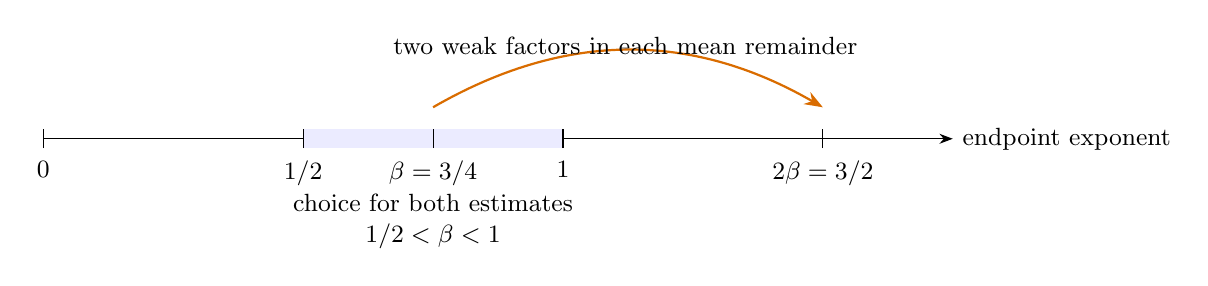
\begin{tikzpicture}[x=6.6cm,y=1cm,font=\small,>=Stealth]
\draw[->] (0,0)--(1.75,0) node[right] {endpoint exponent};
\fill[blue!8] (.5,-.12) rectangle (1,.12);
\foreach \x/\lab in {0/0,.5/{1/2},.75/{\beta=3/4},1/1,1.5/{2\beta=3/2}}
 {\draw (\x,-.12)--(\x,.12); \node[below] at (\x,-.16) {$\lab$};}
\draw[->,thick,orange!85!black] (.75,.4) to[bend left=30] (1.5,.4);
\node[above] at (1.12,.95) {two weak factors in each mean remainder};
\node[align=center] at (.75,-1.05) {choice for both estimates\\$1/2<\beta<1$};
\end{tikzpicture}
\caption{The choice $\beta=3/4$ serves two estimates. Neighboring
exponents below one control the reference inverse. The mean equations
multiply two weak factors and produce an exponent above one, giving
the strengthened metric bound in Theorem~\ref{thm:new-annular-height}.
Flat extension already follows from any positive exponent.}
\label{fig:exponent-gain}
\end{figure}

\subsection{The annular conclusion}

\begin{theorem}[A nonradial height with flat ends]
\label{thm:new-annular-height}
For the fixed reference of Proposition~\ref{prop:rad-fixed-theorem}
there is $q_0>0$ and a smooth branch
$(u_q,\nu_q,\kappa_q,h_{L,q})$, $|q|<q_0$, through
$(\Phi_*,0,0,\id)$, with the following properties.
Set $w_q=w_*e^{\nu_q\chi_*+\sum_m\kappa_{q,m}\chi_m}$ and
$z_q=h_{w_q}+qu_q$, choosing a fixed additive normalization for
$h_{w_q}'=w_q$. Then
\[
 \mathcal N_{h_{w_q}}(z_q)=0,\qquad
 |dz_q|_{(1+w_q^2)dr^2+r^2d\theta^2}<1,\qquad \ell_*u_q=1.
\]
The profile is positive in the annular interior and extends smoothly
by zero across both endpoints. The height is even and $\pi$-periodic
in angle, extends smoothly by a constant at each endpoint, and is
nonradial for $q\ne0$. The two constants may differ.
All roots of $w_q'$ and their radial germs agree with the reference.
The two characteristic returns of the true height derivative obey
\begin{equation}\label{eq:annular-return-condition}
 h_{R,q,m}f_{q,m,\pm}h_{L,q,m}^{-1}=R_{\pm T_m}
\end{equation}
for increasing odd $\pi$-equivariant charts and the fixed reference angles.
On the same interval of $q$, for every $s$,
\begin{equation}\label{eq:annular-branch-estimates}
 \|u_q-\Phi_*\|_{\mathcal X_\beta,s}\le C_s|q|,\qquad
 |\nu_q|+\|\kappa_q\|_{\mathcal K_{2\beta},s}\le C_sq^2.
\end{equation}
The branch is smooth with these topologies. In particular, for
every $a\ge0$ and $\epsilon>0$,
\[
 |\partial_r^a(w_q-w_*)|\le C_{a,\epsilon}q^2H^{1-\epsilon}
\]
at the endpoints, and $w_q-w_*=O(q^2)$ in every smooth norm.
\end{theorem}

\begin{proof}
The weak branch was constructed in Section~\ref{sec:solving-the-equation}.
Equations \eqref{eq:rewrite-mean-recovery} and
\eqref{eq:rewrite-control-recovery} give the strengthened estimates
and smooth dependence just proved. Choose $q_0$ so that
$[-q_0,q_0]$ lies inside its domain. Every seminorm of this smooth
branch is bounded on that one compact interval; the constants depend
on the order, but $q_0$ does not.

On the tails the compact control vanishes. Differentiating the
formula for $w_q$ gives
$|\partial_r^a(w_q-w_*)|\le C_aq^2H^{2\beta}E_0^{C_a}$.
Since $2\beta>1$, \eqref{eq:full-material-envelope} implies the
displayed endpoint estimate. In the compact middle use smoothness
and the quadratic bound for $\nu_q$. All controls vanish near each
turning circle, preserving its full metric germ; the common low
neighborhood preserves the signs elsewhere.

At a zero both residual corrections vanish. The exact return
identities for $\widehat L$ therefore hold for the true derivative.
The common inequality $D>0$ is equivalent to $|dz_q|_g<1$.
The scalar residual vanishes, and the curvature formula identifies
this with flatness of $g-dz_q^2$. Since $\ell_*u_q=1$, the second
angular component is nonzero, so $z_q$ is nonradial for $q\ne0$.

The height space already gives a flat extension after subtracting
its endpoint constants, including all parameter derivatives.
Extend $w_q$ by zero and $z_q$ by those constants and enlarge the
annulus slightly. The enlarged annulus has zero-profile open collars around its
original positive-profile core. The remainder metric stays positive
and flat on these collars, giving the data needed for geometric
closure. This proves the theorem.
\end{proof}

\subsection{Fixing the metric and moving the surface}

We finish by distinguishing the two parameters. The small parameter
$q$ was used to construct one nonradial realization of one rotational
metric. Choose a sufficiently small nonzero value and keep it fixed.
The annular theorem then supplies exactly the data of
Theorem~\ref{thm:geometric-closure}: a positive flat metric
$g-dz_q^2$, the half-turn symmetry, and two constant-height collars.

That theorem develops the graph, fills its inner disk, and attaches
the fixed marked complementary cap. Its independent phase parameter
$\tau$ gives the jointly smooth periodic family
\[
 F_\tau(r,\theta)=R_{-2\pi\tau}F(r,\theta+2\pi\tau)
\]
on the moving annulus and the fixed map elsewhere. The collars cancel
the two rotations pointwise. The marked cap makes two resulting
closed images noncongruent. The same geometric theorem proves
embeddedness, constant area, constant enclosed volume and constant
total oriented mean curvature. This proves Theorem~\ref{thm:main}.

\appendix
\section{Why a finite angular ansatz does not close}
\label{app:app-obstructions}

Section~\ref{sec:scalar-core} ruled out a monotone flat end for the
linearized height. A different tempting simplification is to keep a
finite number of angular modes in the nonlinear height. The
obstruction below explains why the inverse must accommodate all even
frequencies, even though its initial seed has only frequency two.
It is independent of the existence argument.

\begin{proposition}\label{prop:obs-finite-square}
Let $E>0$ be $C^1$ on a connected interval $I\subset(0,\infty)$.
If a real $C^2$ solution of the Darboux equation for
$E\,dr^2+r^2\,d\theta^2$ satisfies
\[
 z^2=\sum_{|j|\le J}b_j(r)e^{ij\theta},\qquad
 b_{-j}=\overline{b_j},\qquad b_j\in C^2(I),
\]
and is radial on a nonempty open radial interval, then it is radial
throughout $I$. This includes every finite Fourier height, and every
smooth square root of a finite trigonometric polynomial.
\end{proposition}

The issue is continuation through a zero of a Fourier coefficient.
A nonzero coefficient has a complex phase, so a real-valued
uniqueness argument would not suffice. We give the continuation
argument rather than assume that the resulting singular ordinary
differential equation has ordinary uniqueness.

\begin{proof}
Set $v=z^2$ and $K=E'/(2rE^2)$. The Hessian identity
$\nabla^2v=2z\nabla^2z+2dz\otimes dz$, together with the
two-dimensional rank-one determinant identity, gives
\begin{equation}\label{eq:obstruction-polynomial}
 2v\det_g\nabla^2v-\operatorname{cof}_g(\nabla^2v)[dv,dv]
       =8Kv^2-2Kv|dv|_g^2.
\end{equation}
To check it without dividing by $z$, expand the two terms on the
left: the terms containing
$z^3\operatorname{cof}_g(\nabla^2z)[dz,dz]$ cancel, leaving
$8z^4\det_g\nabla^2z$. Substitution of the Darboux equation
gives the right side. Thus the identity also holds where $z=0$.

Let $b=b_J$ for the highest positive frequency $J$, and put
$a=EJ^2/r$, $d=E'J^2/(2r)$. The coefficient of frequency $3J$
in \eqref{eq:obstruction-polynomial} contains only three copies
of $b$. It is
\begin{equation}\label{eq:obstruction-highest-mode}
\begin{split}
0={}&(2bb'-ab^2)b''-(b')^3+ab(b')^2
 -\frac{2a}{r}b^2b'+\frac{2a}{r^2}b^3\\
 &\quad+db^2b'-\frac{2d}{r}b^3.
\end{split}
\end{equation}
For a direct coefficient check, write the three Hessian entries of
$v$ as
$A=v_{rr}-E'v_r/(2E)$,
$B=v_{r\theta}-v_\theta/r$,
$C=v_{\theta\theta}+rv_r/E$.
After multiplication by $Er^2$, the left side is
$2v(AC-B^2)-(Cv_r^2-2Bv_rv_\theta+Av_\theta^2)$.
Replace the jets by $b,b',b'',iJb,iJb',-J^2b$ and collect
terms; the quadratic term on the right has no frequency $3J$.

On a component where $b\ne0$, take a continuous complex square root
$y^2=b$. Substitution reduces \eqref{eq:obstruction-highest-mode} to
\begin{equation}\label{eq:obstruction-square-root}
 (4y'-ay)y''+a(y'-y/r)^2+d(yy'-y^2/r)=0.
\end{equation}
Fix a compact subinterval and $K_1>1+\sup|a|$. The quantity
\[
 U=\max(K_1|y|,|y'|)
   =\max\left(K_1\sqrt{|b|},
                    \frac{|b'|}{2\sqrt{|b|}}\right)
\]
satisfies $|U'|\le CU$ almost everywhere. Indeed, where the second
term is larger, $|4y'-ay|\ge3|y'|$, and
\eqref{eq:obstruction-square-root} gives $|y''|\le C|y'|$.
Where the first is larger, its derivative has absolute value at
most $K_1|y'|\le K_1U$. The maximum is locally Lipschitz,
so the same estimate holds through its switching points.
It bounds $U$ both above and away from zero at every finite
endpoint of a nonzero component.

At a zero of $b$, \eqref{eq:obstruction-highest-mode} gives
$b'=0$. At a finite endpoint of a nonzero component, $y\to0$,
so $U=|y'|$ nearby. The estimate for $y''$ yields a limit
$y'\to\lambda\ne0$, and consequently
\begin{equation}\label{eq:obstruction-quadratic-zero}
 b''=2(y')^2+2yy''\longrightarrow2\lambda^2\ne0.
\end{equation}
Thus such an endpoint is an isolated quadratic zero. Across it
$U$ has the continuous value $\sqrt{|b''|/2}$ and the same
differential bound.

Consider the open set
$\mathcal O=\{b\ne0\}\cup\{b=0, b''\ne0\}$.
If a component of $\mathcal O$ had an interior boundary point,
then $b=b''=0$ there. An infinite accumulation of quadratic zeros
would contradict the positive lower bound for $U$ and continuity
of $b''$; a last nonzero interval would contradict
\eqref{eq:obstruction-quadratic-zero}. Hence
$\mathcal O$ is either empty or all of $I$. Since $b$ vanishes
on the given open radial interval, it must vanish everywhere.

Remove this highest coefficient and repeat down the finite
expansion. The resulting $z^2$ is radial. At each radius a real
continuous function on the connected circle whose square is
constant is itself constant. Therefore $z$ is radial.
\end{proof}

This result does not say that a single angular mode is useless.
It is exactly the right seed for the linearized construction.
It says that the nonlinear completion cannot be confined to a
finite angular ansatz once it is required to meet a radial collar.

\section*{Use of AI}
\addcontentsline{toc}{section}{Use of AI}
AI systems assisted with mathematical exploration, writing,
algebraic verification and critical reading. Separate AI readers
were used to review the manuscript; their reports are revision
records, not human peer review. The author is responsible for the
mathematical claims and their presentation.

\bibliographystyle{plain}
\bibliography{references}
\end{document}
